
% \begin{abstract}
% Selecting appropriate thresholds for anomaly detection in online, unsupervised settings is a challenging task, especially in the presence of data distribution shifts. Addressing these challenges is critical in many practical large scale systems, such as infrastructure monitoring and network intrusion detection.
% %
% This paper proposes an algorithm that connects online thresholding with constructing confidence sequences achieving (1) adaptive online threshold selection robust to distribution shifts, (2) statistical guarantees on false positive and false negative rates without any distributional assumptions, and (3) improved performance when given relevant offline data to warm-start the online algorithm, while having bounded degradation if the offline data is irrelevant. We complement our theoretical results with empirical evidence that our method outperforms commonly used baselines across synthetic and real world datasets.
% \end{abstract}

% Choosing a threshold on anomaly scores to classify if a given data point is an anomaly is an important problem. This challenge is exacerbated in the online setting when the anomaly detector is unsupervised and the data-stream undergoes distribution shift. Both of these are common in many practical large scale systems, including those for detecting performance anomalies in computer systems, infrastructure monitoring and network intrusion detection.
% In this paper, we connect the online thresholding problem to that of constructing online confidence sequences. By on this connection, we present an algorithm that can select anomaly thresholds automatically, with guarantees on false positive and false negative rates without making any distributional assumptions. Furthermore, we prove that our algorithm is adaptive to distribution shifts, and can leverage offline data to further improve its performance.
% Ours is the first algorithm for online anomaly thresholding with rigorous statistical guarantees. We complement our theoretical results by showing empirically that our method outperforms commonly used heuristics across a variety of academic and real world datasets.


\section{Introduction and Motivation} 
Online anomaly detection (OAD) is the task of identifying deviations from the normal behavior in a streaming fashion, where samples arrive sequentially, and decisions must be made before the next sample is received. This task plays a fundamental role in various practical applications within cyber and cyber-physical systems, including maintenance \cite{khan2020industrial}, monitoring \cite{hill2010anomaly}, and security \cite{mirsky2018kitsune, lazarevic2003comparative}. In modern environments, the sheer volume and velocity of data make it often impractical to have comprehensive labels for all anomalous samples \cite{siffer2017anomaly, schmidl2022anomaly, ren2019time, audibert2020usad}.

In deployment, typical AD algorithms assign a real-valued anomaly score to each sample, where a higher score indicates a greater degree of anomaly \cite{chandola2009anomaly}. The OAD algorithm first scores each sample and then calibrates a threshold to make the binary decision of whether the given sample is anomalous or not. The choice of this threshold is critical due to its significant downstream impact. In security systems, for example, failing to detect a genuine anomaly or security event can have catastrophic consequences \cite{203674}. Conversely, false positives incur costs, as each detection necessitates investigation by a security operator, potentially leading to `alert fatigue' \cite{202751, lin2018collaborative, he2023cloudshield}.

Given the risk of incorrect decisions, a common methodology to set the threshold is by \emph{abstaining} from decisions for an initial `cold-start' number of samples on the  stream \cite{10.14778/2850583.2850593, katz2023cold}. At the end of the cold-start period, a threshold is chosen for future decision making, either by algorithm or by an expert based on the online scores during the cold-start, as well as any offline data that is available \cite{ren2019time, bhatia2021mstream,huang2022semi, li2021fluxev}. 
This approach has two drawbacks. 
Firstly, using a fixed cold-start duration across all streams independent of stream statistics is sub-optimal and can lead to much more abstains than necessary. Secondly, a static threshold is prone to performance loss when the data stream undergoes distribution shift - a common occurrence in many AD systems \cite{279982,gama2014survey}. Although adapting anomaly scoring to distribution drifts have been studied \cite{ma2018robust,bhatia2022memstream, sankararaman2022fitness}, limited advances have occurred in adapting the threshold dynamically.
%We frame the threshold selection as online quantile estimation and provide guarantees on number of false positives and false negatives that hold even under distribution shifts and provably improve in the presence of offline data. 
%
%scores gathered thus far  (cf. Fig \ref{fig:static_cold_start}). If appropriate, offline data is used along side the online scores during cold-start to minimize risks of incorrect decisions \cite{ren2019time, bhatia2021mstream,huang2022semi, li2021fluxev}. 


%\subsection{Threshold selection as quantile estimation}

We formulate adaptive threshold selection as online quantile estimation by defining anomalies as tail quantile of anomaly scores \cite{steinwart2005classification, cadre2013estimation, gan2017scalable, siffer2017anomaly}. Formally, we model that each time $t \in \mathbb{N}$, the anomaly score $S_t \in \mathbb{R}$ is independently sampled from distribution $f_t$. This score $S_t$ is an {anomaly} if it exceeds the $p$th quantile of the distribution $f_t$. We assume the quantile level $p \in (0,1)$ is known, while the distribution $f_t$ as unknown to the algorithm. 
Knowledge of $p$ arises either from a constraint on the rate of anomalies that can be investigated without succumbing to alert fatigue \cite{hassan2019nodoze, ho2021hopper}, or from domain knowledge \cite{perini2023unsupervised}. 

Performance of threshold selection is measured by false positives (FP), benign samples marked as anomalous, false negatives (FN), anomalous sample mark as benign, and number of samples abstained from making a decision on. Since AD outputs are typically used to make consequential decisions, e.g. engaging human operators to triage alerts, OAD systems must achieve low number of FPs and FNs, by possibly trading-off with abstains \cite{ho2017detecting}. Further, these systems need to be adaptive to distribution shifts and be designed without requiring distributional assumptions (cf. \emph{Research challenges} $5$-$7$ of \cite{sadik2014research}).

 \subsection{Desiderata of OAD threshold selection systems}
 \label{sec:desiderata}

% AD Threshold systems marks each sample as either anomalous, non-anomalous or abstains from decision making \cite{chandola2009anomaly}. Performance is measured by false positives (FP), benign samples marked as anomalous, and false negatives (FN), anomalous sample mark as benign, in addition to number of samples abstained on. Typically, since AD outputs are used to make consequential decisions, e.g. engaging human operators to triage alerts, OAD systems must have low number of FPs and FNs achieved at the cost of abstains \cite{ho2017detecting}. Further, these systems need to be adaptive to distribution shifts and be designed without requiring distributional assumptions (cf. \emph{Research challenges} $5$-$7$ of \cite{sadik2014research} and references therein). In summary, the following set of statistical requirements are desired.

 %the following set of statistical requirements desired for online threshold selection. \cite{sadik2014research}.
 
In summary, the following set of statistical requirements is desired for online threshold selection.
 
    \emph{\textbf{(i) High accuracy:}} Constant number of mistakes\footnote{Throughout, we denote the mistakes as sum of FP and FN.} independent of the stream length on an i.i.d. data-stream.

      \vspace{-1mm}
     \emph{\textbf{(ii) Low abstention:}} Abstain on a vanishing fraction of samples on an i.i.d. stream, i.e. small cold-start period. 

     \vspace{-1mm}
    \emph{\textbf{(iii) Adaptive to distribution changes:}} On a non-stationary stream, number of mistakes and abstains only increase compared to the stationary setting by a constant factor that is independent of the stream length, but only proportional to the number and magnitude of distribution changes. 
    
    \vspace{-1mm}
       \emph{\textbf{(iv) Learn from offline dataset:}} When unlabeled offline datasets are available, abstain rate is a constant independent of stream length, as long as the online distribution matches one of the offline distribution. In the worst-case of arbitrary offline dataset distribution, performance degradation compared to no offline dataset must be bounded independent of stream length and size of the dataset.

       \vspace{-1mm}

       \emph{\textbf{(v) Distribution and parameter free:}} The algorithm does not require any knowledge of the distributions or assumptions such as sub-gaussian tails or parameterized distribution family, and nevertheless must guarantee all of above.
     %The algorithm however does not know apriori if the online stream and offline dataset are from the same distribution.
% \begin{enumerate}[itemsep=0pt,topsep=-2pt, labelindent=-1pt,labelwidth=!]
%     \item \textbf{High accuracy:} Constant, independent of the stream length, number of mistakes\footnote{Throughout, we denote the mistakes as sum of FP and FN.}, on an i.i.d. data-stream.
%     \item \textbf{Low abstention:} Abstain on a vanishing fraction of samples on an i.i.d. stream, i.e., small cold-start period. 
%     \item \textbf{Adaptive to distribution shifts:} On a non-stationary stream, the FPs, FNs and abstains only increase compared to the stationary setting by a constant factor that is independent of the stream length, but only proportional to the number and magnitude of distribution changes. The algorithm however cannot know apriori the number of changes on the stream.
%     \item \textbf{{\color{black} Learn from offline data:}} If there is access to multiple unlabeled offline datasets, then the fraction of abstains is a constant independent of stream length, whenever the online distribution matches one of the offline distribution. However, if none of the offline distributions matches the online stream, the performance must be comparable to the setting without offline data. %The algorithm however does not know apriori if the online stream and offline dataset are from the same distribution.
%     \item \textbf{Distribution and parameter free:} The algorithm does not require any knowledge of the distributions or assumptions such as sub-gaussian tails or the distribution family being parameterized, nevertheless must guarantee all of the aforementioned performance.
% \end{enumerate}

%Crucially, we want the above desiderata to be satisfied without any assumptions on the distribution such as tails or parametric form. 




%The online version of the unsupervised AD problem is one where samples are presented to the AD algorithm one at a time in a streaming fashion. At each time step, the AD algorithm outputs an anomaly score based on the samples seen thus far. As the problem is unsupervised, the ground-truth label of the sample is not available to the AD algorithm before making its next set of predictions. This unsupervised, OAD is a common abstraction for many problems in cloud-computing, performance monitoring and network intrusion detection systems .

%Typical performance measures of anomaly detection algorithms are AUC (Area under the curve) of the ROC (Receiver operating curve). This measure is computed by comparing the anomaly scores output by the AD algorithm and the ground-truth binary labels by sweeping over all possible choice of anomaly thresholds. However, 

% \paragraph{Anomaly thresholding.}  Most modern AD algorithms outputs an anomaly score for a given sample and are evaluated using threshold-agnostic metrics such as AUCROC. The choice of how to choose a threshold is often left unstudied and unreported. This is especially surprising since in practice, tuning thresholds is an important problem and critical to the performance of any AD system \cite{chandola2009anomaly, hundman2018detecting} 


\subsection{Main result and technical contributions}

{Algorithm \ref{alg:five} is distribution and parameter free and is the \emph{first algorithm to satisfy all the aforementioned desiderata.}}  Algorithm \ref{alg:five} does not require knowledge on the locations or number of distribution shifts nor on the online stream or the offline datasets' distributions. Nevertheless, under mild technical assumptions, the guarantees in Theorem \ref{thm:core_theorem} show that the performance adapts to the problem complexity.
%, if any stationary segment of the online stream matches any of the offline datasets' distirbution, the number of abstains and mistakes are small. On the other hand if a stationary segment in the online distribution is arbitrary and does not match any offline datasets' distribution, then the performance on this segment is comparable to one in which no offline data is present.
%However, the algorithm does not need as input any prior information, but rather its performance adapts to the complexity of the online data stream. 
%In particular, FP, FN and abstain are lower when there is fewer distribution shifts and/or offline datasets have the same distribution as the online stream, with the bounds naturally identifying the problem complexity parameter. 
%\subsection{Technical Contributions}
Concretely, our contributions are as follows.

{\color{black} \textbf{1. High accuracy requires abstention.} We prove that any  scheme that does not abstain,  cannot achieve constant FPs and FNs, even for a stationary stream. The proof follows by constructing a hard instance and a reduction from decision making to hypothesis testing on that instance. }

{\color{black} \textbf{2. Algorithm using confidence sequences (CS) to adapt threshold to distribution changes.} 
%  Threshold using confidence sequence (CS) to be adaptive to changes in distribution.
%We connect OAD and threshold selection with confidence sequences (CS). 
%We use  CS to make decisions to yield high-accuracy and a data-dependent abstain. 
A sample $S_t$ is deemed as an anomaly by our algorithm (Algo. \ref{alg:five}) if it exceeds the upper confidence of the $p$th quantile,  is benign if it is smaller than the lower confidence, and is abstained from otherwise (Fig. \ref{fig:motivation_alg_1}). The crux of our algorithm is in choosing the \emph{relevant online and offline samples} to construct the CS. Online distribution shifts are detected by constructing CS on different sub-sequences and testing if they have a non-empty intersection. Theorem \ref{the:iid} shows that on an i.i.d. stream of length $T$, no mistakes  and at-most $\mathcal{O}(\sqrt{T})$ abstains occur with high probability. 
%3. \textbf{Confidence sequences can provably be adaptive to distribution shifts.} 
Theorem \ref{thm:online_shift} shows that when there are distribution shifts, our algorithm incur total additional mistakes \emph{independent} of $T$, without requiring any knowledge of the data distributions or change-points.
%our algorithm, without requiring any knowledge of the distributions or change-points, incurs an additional factor \emph{independent} of $T$ mistakes and abstains compared to the stationary stream.

% The CS for the $p$th quantile is a sequence of random intervals $([l_t, u_t])_{t \geq 1}$ such that for all $t \geq 1$, {\em(i)} $l_t \leq u_t$ almost-surely are measurable functions of $S_1, \cdots, S_t$, and {\em(ii)} with high probability, the intersection of all intervals contains the true quantile \cite{howard2022sequential}. 
% %The existence and construction of CS  are shown in \cite{howard2022sequential}. 
% Algorithm \ref{alg:five} declares $S_t$ anomalous if $S_t > u_t$, benign if $S_t < l_t$ and abstain otherwise (Figure \ref{fig:motivation_alg_1}). Distribution shifts are detected in Algorithm \ref{alg:five} by constructing CS on different sub-sequences and testing if they have a non-empty intersection.  Theorem \ref{the:iid} shows that on an i.i.d. stream of length $T$, no mistakes  and at-most $\mathcal{O}(\sqrt{T})$ abstains occur with high probability. 
% %3. \textbf{Confidence sequences can provably be adaptive to distribution shifts.} 
% Proposition \ref{prop:dist_changes} shows that on a non-stationary stream, the mistakes and abstains only increase by a constant factor depending on the magnitude of distribution shifts, while Algorithm \ref{alg:five} does not require any knowledge of the distributions.

\textbf{3. Relevant offline dataset improves online performance, while irrelevant offline dataset has bounded degradation.} Theorem \ref{thm:core_theorem} proves that when offline data matching the distributions of the online stream are available, they improve abstain rate without loss of accuracy. In the \emph{worst-case} when the offline dataset's distributions are arbitrary, the performance degradation compared to the case when the algorithm ignores offline dataset is \emph{bounded independent of stream length or offline dataset size}. Algorithm \ref{alg:five} does not a priori know if the offline dataset is useful or not, but yields improved guarantees whenever the offline dataset is useful. The technical novelty is to rely on an offline dataset \emph{only if a CS constructed on offline dataset} intersects with the online CS. This is the first algorithm for online thresholding showing improved  performance in the presence of useful offline data, while guaranteeing worst-case bounds if the offline data is arbitrary. 
%Previous methods for this only relied on heuristics \cite{audibert2020usad, bhatia2022memstream, huang2022semi} 

%4. \textbf{Empirical.} Superior performance in terms of FP, FN and abstains compared to baselines and heuristics, both on real and synthetic data.

}

%\vspace{-0.5em}
% \paragraph{1 and 2. High Accuracy and Low Abstention : Confidence-sequences as adaptive cold-start.} Our primary contribution is to make rigorous the connection between OAD and threshold selection with confidence sequences (CS). The CS for the $p$th quantile is a sequence of random intervals $([l_t, u_t])_{t \geq 1}$ such that for all $t \geq 1$, {\em(i)} $l_t \leq u_t$ almost-surely are measurable functions of $S_1, \cdots, S_t$, and {\em(ii)} with high probability, the intersection of all intervals contains the true quantile \cite{howard2022sequential}. 
% %The existence and construction of CS  are shown in \cite{howard2022sequential}. 
% Given a CS, Algorithm \ref{alg:five}  makes decisions on an i.i.d. sequence by declaring a sample $S_t$ anomalous if $S_t > u_t$, benign if $S_t < l_t$ and abstain if $l_t \leq S_t \leq u_t$ (Figure \ref{fig:motivation_alg_1}). We show in Theorem \ref{the:iid} that our algorithm guarantees that there are $0$ FP and FN and at-most order $\sqrt{T}$  abstains over $T$ samples, with high probability. 

% \vspace{-0.5em}
% \paragraph{3. Adaptivity to distribution shifts.} We use the CS to also detect distribution shifts, by deeming a shift to have occurred if the CS on two sub-sequences of points $S_1, \cdots, S_t$ are non-intersecting \cite{shekhar2023sequential, sankararaman2023online}. Our result in Proposition \ref{prop:dist_changes} shows, that the number of FPs and FNs only scale with the number of distribution shifts, even when the algorithm has no knowledge of the number and location of distribution changes.

%\vspace{-0.5em}
%\paragraph{4. Efficiency: Provably improving online performance in the presence of offline datasets.} 
%Our most general result is in Algorithm \ref{alg:five} whose performance guarantee is stated in Theorem \ref{thm:core_theorem}. This general result assumes that at each time, in addition to all the samples on the stream observed thus far, the AD system also has access to a \emph{offline dataset}. 
% In Theorem \ref{thm:core_theorem}, we prove that when an offline dataset is available, the following two desiderata can be achieved \emph{simultaneously}. If the online stream has the same distribution as one the offline datasets, then improved performance in terms of FP, FN and abstain are observed as opposed to not using the offline data, and if the online stream's distribution does not match any offline dataset, then the performance is comparable to the performance in the absence of any offline dataset. In particular, Theorem \ref{thm:core_theorem} proves that desiderata $4$ from Section \ref{sec:desiderata} is achieved by Algorithm \ref{alg:five}. The algorithmic novelty is to rely on an offline dataset only if a CS constructed on offline dataset intersects with the online CS. This is the first provable strategy of improved thresholding performance in the presence of offline data, while methods relied on heuristics \cite{audibert2020usad, bhatia2022memstream, huang2022semi} 

%that using an offline dataset is algorithmicaly similar to detecting a change-point, namely the online stream matches the offline if the CS from the offline and online stream overlap. 

%This setting is also of practical importance as it is a common occurrence in AD systems in several cloud-computing and IoT settings \cite{sauvanaud2018anomaly,islam2021anomaly, 235002}. However, our results are the first provable algorithm with guarantees on FP, FN and the number of abstains.  \abishek {Flex on how theory is SOTA.}

\begin{figure}
\centering
\begin{subfigure}{.48\columnwidth}
  \centering
  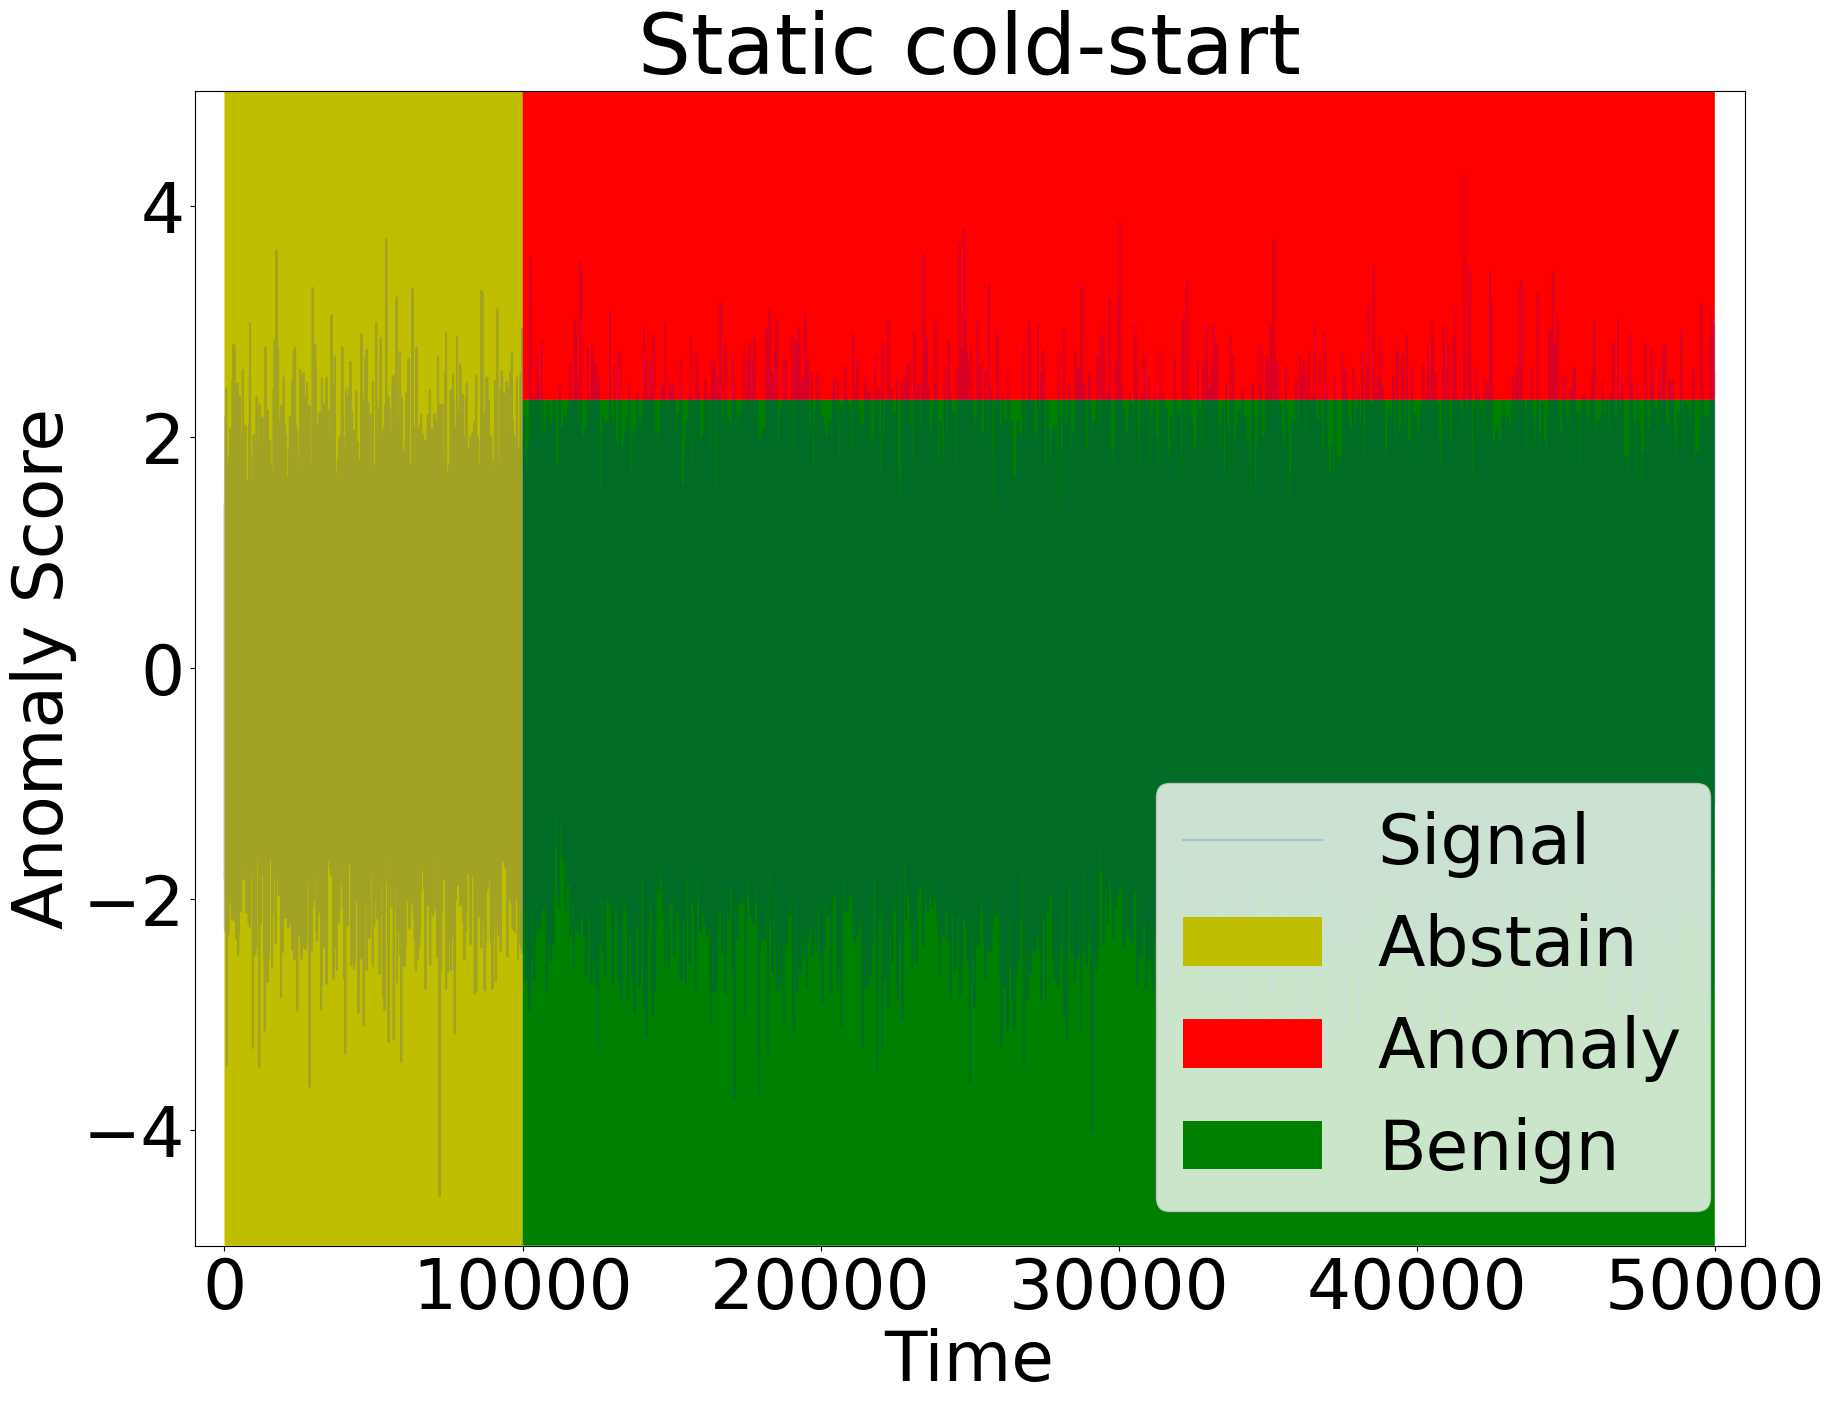
\includegraphics[width=\linewidth]{anomaly/figs/static_cold_start.png}
  %\caption{Anomaly threshold set using a fixed cold-start period}
  \caption{}
  \label{fig:static_cold_start}
\end{subfigure}%
\begin{subfigure}{.48\columnwidth}
  \centering
  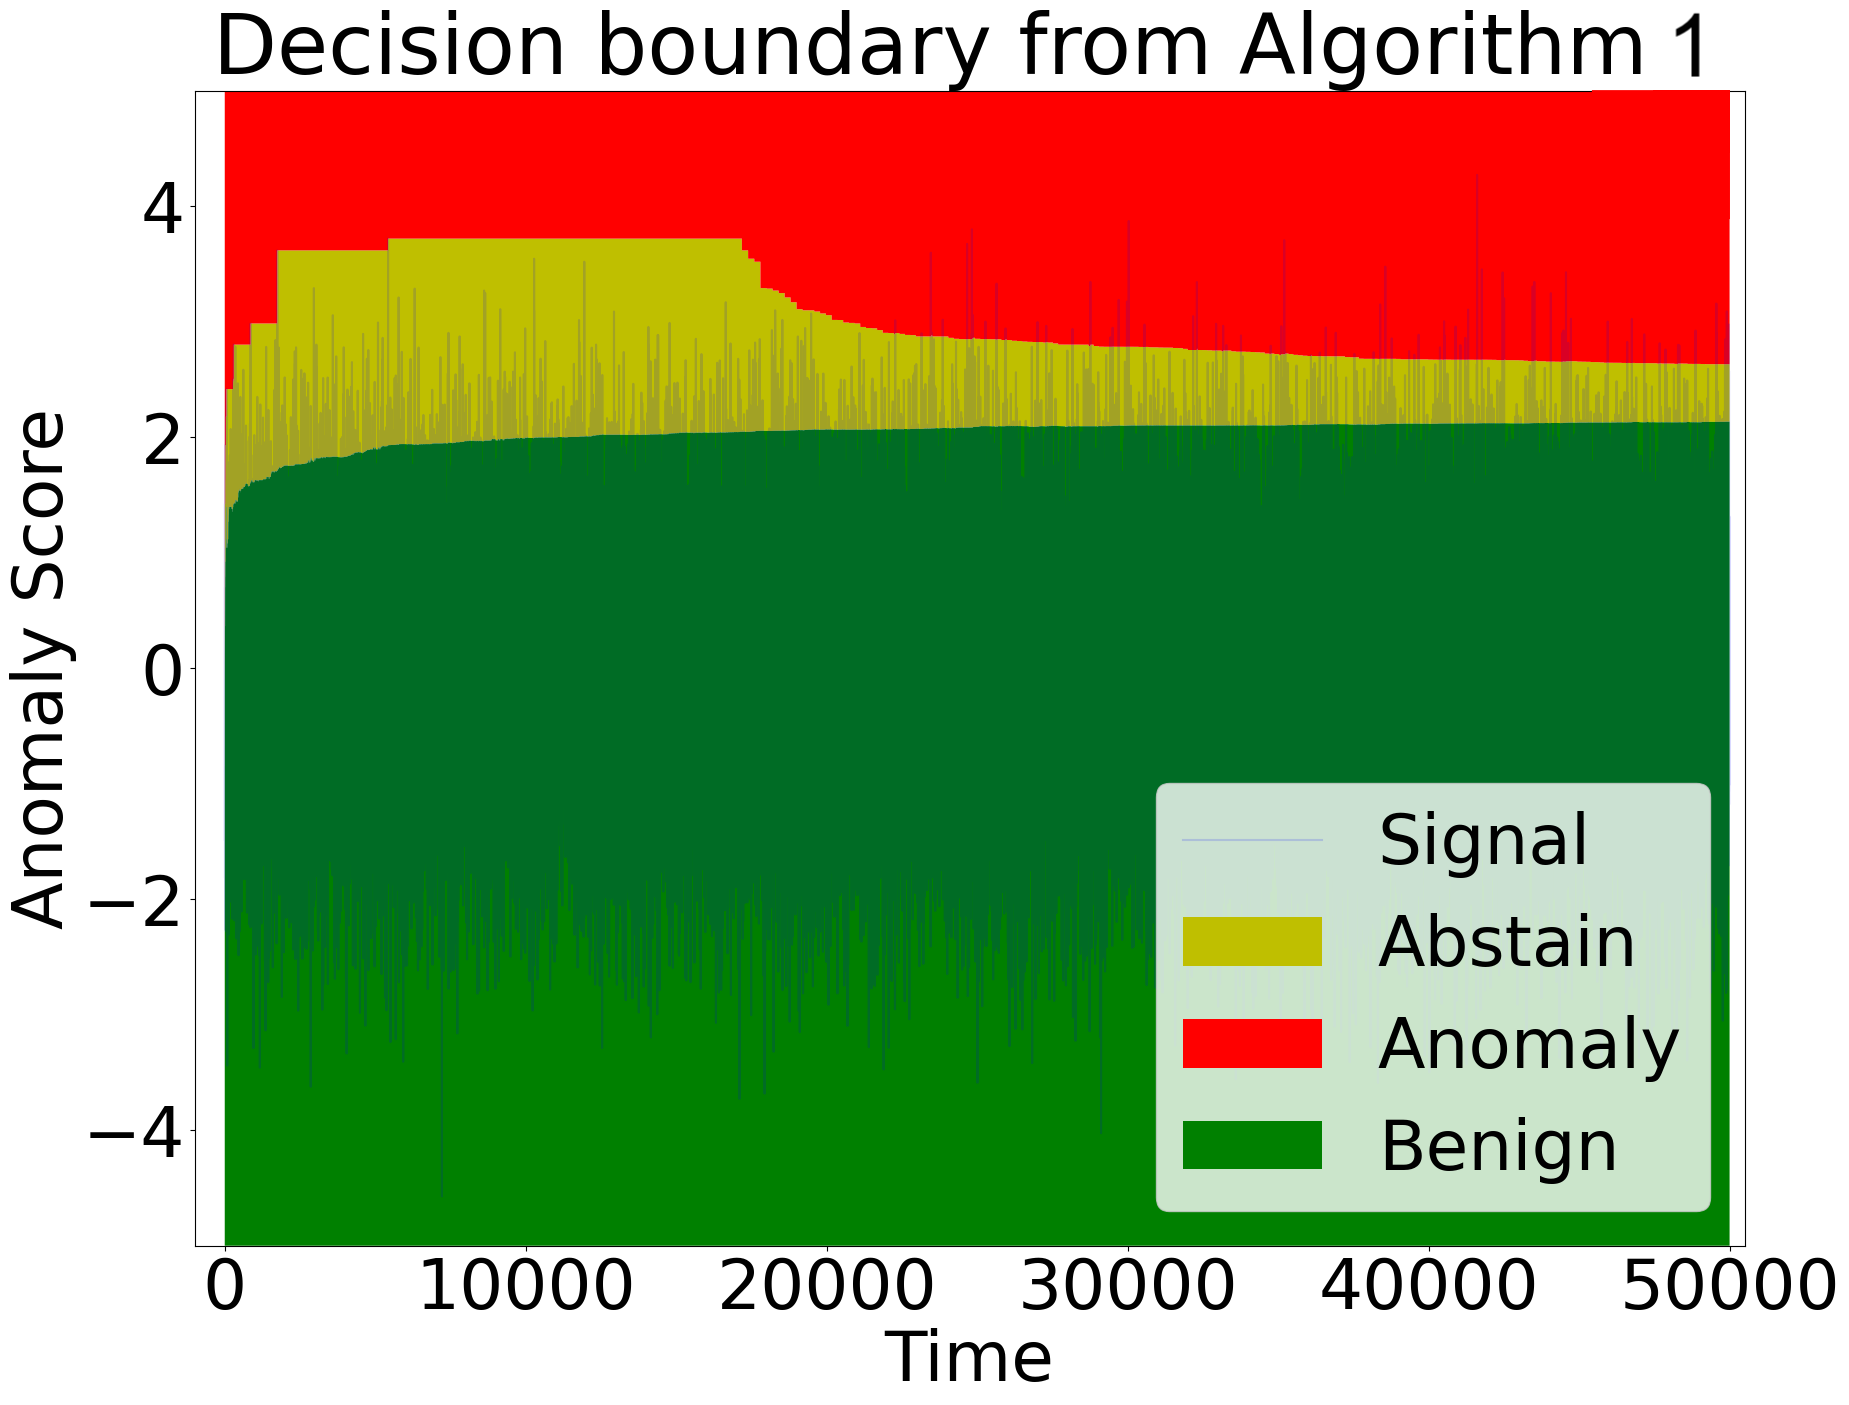
\includegraphics[width=\linewidth]{anomaly/figs/algo1_example.png}
  %\caption{A subfigure}
  \caption{}
  \label{fig:sub2}
\end{subfigure}
\vspace{-0.5em}
\caption{Fig $(a)$ is the heuristic of a fixed cold-start where all samples are abstained from and a static threshold for all future samples. Fig $(b)$ is the decision boundary from Algorithm \ref{alg:one} using an adaptive cold-start.}
\label{fig:motivation_alg_1}
\vspace{-1.5em}
\end{figure}





% AD algorithms abstain by relying on an initial cold-start period. At the end of the cold-start period, the AD system will use the samples seen and any offline information to choose an appropriate threshold \cite{audibert2020usad, chandola2009anomaly}. 




% We introduce abstaining as a possible output of an AD algorithm, in addition to the canonically binary output of anomaly and benign data. The abstain option can be viewed as a data-adaptive, more flexible framework of the cold start period that is commonly used to tune the anomaly threshold. In this paper we include abstaining into the regret metric, to analyze its trade off with making false positive and false negative errors.  

% \paragraph{Leveraging offline datasets to improve online performance, provably}


% \paragraph{Finite-sample, distribution free guarantees on performance}

% \paragraph{Contributions} We are the first work to systematically study the problem of unsupervised anomaly thresholding. We propose algorithms in various settings, and provide a principled framework to analyze their performance. Our contributions are: 

% \begin{enumerate}
% \item {\color{red} Our method provides a statistical framework to tune anomaly thresholds in an online fashion. Our methodology picks a `cold-start' period that is data dependent. Anomalies that are harder to distinguish have a larger cold-start than those that are easier to distinguish.
% Thus, our methodology gives a principled generalization of the common heuristic of having a fixed cold-start period. }
%     %\item Our algorithm improves upon the manually tuned anomaly thresholding with cold-start period commonly used in practice, and provide an algorithm where abstaining is adaptive and data-dependent.
%     \item We prove guarantees on false positive and false negative rates, and number of abstains. {\color{red} 1-2 sentences on the novelty/difficulty}
%     \item We prove that our algorithms and guarantees are adaptive to online distribution shifts. {\color{red}1-2 sentences on how we connect the detection delay with the mistake bounds.}
%     \item Our algorithms leverages offline data to improve online performance with best of both worlds results: it significantly lowers number of abstains when offline data is available, and reduces to online algorithm when it is not. {\color{red} Our algorithm is the first to rigorously show the best of both worlds for online threshold selection?}
% \end{enumerate}

%Our work shows how to tune parameters to achieve. We also show conditions when presence of offline data can improve online performance.....



% \section{Related Work}%\vspace{-0.5em}
% \paragraph{Dynamic thresholding for AD.} AD is an extensively researched topic, where a common paradigm is to first model data likelihood and then use a threshold to decide if a data point is normal or anomalous. This threshold is typically determined by an expert or empirically, see surveys \cite{luo2021deep, schmidl2022anomaly}. Dynamic and automatic methods makes AD algorithms more practical in real-world deployment \cite{ali2013automated, hundman2018detecting}, and are necessary where the data distribution can shift \cite{siffer2017anomaly}. 

% %\cite{siffer2017anomaly, , hundman2018detecting}
% %This work instead focuses on providing a principled analysis of the thresholding step that follows. Traditionally, and are chosen by heuristics . Works closer to us are thresholding algorithms for univariate online streams .
% %\vspace{-0.5em}
% \paragraph{Confidence Sequences.} We use theoretical results and tools of confidence sequences (CS) for our analysis \cite{ramdas2022game}. \cite{maharaj2023anytime, howard2022sequential} derived the CS algorithm for estimating quantiles online with any-time guarantees, and \cite{shekhar2023sequential} leverages CS's consistency property for detecting distribution shifts. These tools allows us to bound the false positive and negative rates of our algorithm.

% {\color{red} \paragraph{Threshold learning systems.}
% Threshold scores to make the binary decision have been studied in active learning to make the decision of  seeking labels from experts \cite{balcan2007margin, zhang2016online,vishwakarma2023promises}. However, active learning does not have a concept of mistakes and is thus different from ours. 

% }

\section{Notations and Problem Formulation}

We formally state the problem and performance measures.
\vspace{-0.6em}

\subsection{Online Data Stream}
\label{subsec:online_data_stream}

A data-stream of length $T \in \mathbb{N}$ is a collection of $T$, independent, scalar valued random variables $(S_t)_{t=1}^T$, indexed by time $t \in [T]$ \footnote{For any positive integer $L$, we denote $[L] = \{1,\cdots,L\}$}. In practice, $S_t \in \mathbb{R}$ at time $t$ is the \emph{anomaly score} of an input sample produced by an AD algorithm such that high scores corresponds to anomalies.
For each time $t \in [T]$,  $f_t$ is the probability distribution of $S_t$, i.e., $S_t \sim f_t$. We assume $f_t$ is a continuous measure without discrete atoms.\footnote{Formally, $\forall p \in (0,1)$, the set $\{ Q \in \mathbb{R}: \mathbb{P}_{X \sim f}[X \leq Q] = p\}$ has exactly one element.} Since the distribution $f_t$ is indexed by time $t$, $(S_t)_{t=1}^T$ is not necessarily identically distributed and thus non-stationary. We assume that the data-stream although is non-stationary, is piece-wise stationary. 

\begin{definition}(Piece-wise stationary) Let $T$ be the time horizon and let $H_T \leq T-1$ be the total number of change points. Define a set of strictly increasing time indices  $1 < \tau_1 < \tau_2 \cdots < \tau_{H_T}$ as change points; let $\tau_0 = 0$ and $ \tau_{H_T+1} = T$. A piece-wise stationary data-stream $(S_t)_{t=1}^T\sim\Bigl(T,H_T, (\tau_c)_{c=0}^{H_T}, (f^{(c)})_{c=0}^{H_T}\Bigr)$ is such that $\forall k \in [1, H_T]$:
\begin{itemize}[noitemsep,topsep=-2pt,labelwidth=!, labelindent=0pt]
   \item $\forall t \in [\tau_k,\tau_{k+1})$, $S_t \sim f^{(k)}$ are i.i.d. with the $p$-quantile of $f^{(k)}$ denoted as $ Q^{(k)}(p) \in \mathbb{R}$. %Thus, $\forall t \in [\tau_k,\tau_{k+1})$, 
    \item  $f^{(k)} \neq f^{(k+1)}$
\end{itemize}
\label{def:piecewise}
\end{definition}

\begin{figure}[h!]
    \centering
    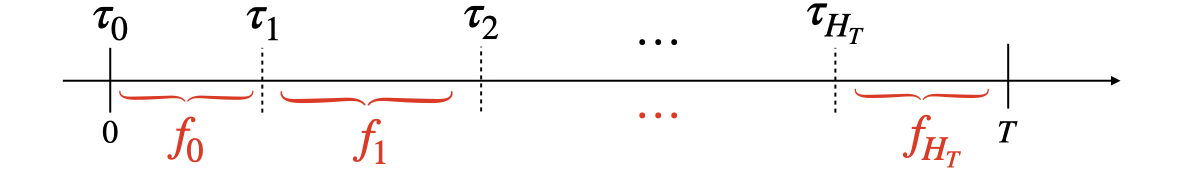
\includegraphics[width=0.9\linewidth]{anomaly/figs/piecewise.jpeg}
    \caption{The piece-wise stationary process}
    \label{fig:enter-label}
    \vspace{-0.8em}
\end{figure}

The special case of $H_T = 0$ corresponds to a stationary i.i.d. data stream.
We remark that our algorithm does not have any information on the change-points  $H_T$, $(\tau_t)_{t=1}^{H_T}$, nor on distributions $(f^{(c)})_{c=0}^{H_T}$. %Nevertheless, the performance  of our algorithm will adapt with the complexity of the data-stream. 

\subsection{Anomaly Definition} 
\label{subsec:anomaly_defn}
%
%As is standard, anomalies are as those time points where the observed sample $S_t$ is larger than the $p$th quantile.
%Following convention \cite{chandola2009anomaly}, we will assume that large values of scores are anomalies. 

\begin{definition}[Anomalies] 
The sample $S_t \sim f_t$ at time $t$ is an anomaly if $S_t > \tau_t$, where $\tau_{t} = \inf \{ \tau\geq 0: \mathbb{P}_{S \sim f_t}[S \leq \tau] \geq p \}$ and $p \in (0,1)$. We denote by $y_t = \mathbf{1}(S_t > \tau_t)$ the indicator variable that the sample $S_t$ is an anomaly.
% \begin{align}
% \begin{split}
%    y_t &= \mathbf{1}(X_t > \tau_{p} ), \text{where} \\
%     \tau_{p} &= \inf \{ \tau\geq 0: \mathbb{P}_{X_t \sim f_t}[X_t \leq \tau] \geq p \}
% \end{split} 
% \end{align} 
\label{def:anomaly}
\end{definition}
%\vspace{-1em}
In words, a sample $S_t$ is anomalous if it exceeds the threshold $\tau_t$ corresponding to the $p$th quantile. Thus, the thresholding algorithm needs to estimate $\tau_t$ and then use that estimate to make the binary decision of whether $S_t$ is an anomaly.
We assume the quantile value $p \in (0,1)$ to be known. 
%In practice, knowledge of $p$ arises, either from constraints on the rate of anomalies that can be investigated \cite{hassan2019nodoze, ho2021hopper}, or from domain knowledge on the base rate of anomalies \cite{perini2023unsupervised}.
% and is thus an extrinsic input.  %While this paper is motivated by anomaly detection and thus focuses on extreme values on one side, but our definitions and algorithms can easily be modified to detect anomaly on both sides, by simultaneously estimating a low and a high quantile.

\subsection{Offline Datasets}
\label{subsec:offline_datasets}

We formalize the notion of \emph{offline datasets} that can be used in addition to using historical samples on the data-stream. Offline datasets are typically available to train the anomaly scoring systems \cite{bhatia2022memstream, audibert2020usad} and have been used to address the cold-start problem in previous works \cite{gutflaish2019temporal,hofmann1999probabilistic}.


 \begin{definition}[Offline Dataset] We define an offline dataset as $K$ sets of independent samples $\mathcal{D} := \{\{X_i^{(j)}\}_{i=1}^{N_j} \}_{j=1}^K$. Each $j \in \{1,\cdots,K\}$ set $\{X_i^{(j)}\}_{i=1}^{N_j}$  are independent samples such that all of the $N_j$ samples are drawn from distributions having the same $p$th quantile denoted by $Q_{(j)}(p)$. A special case is $\{X_i^{(j)}\}_{i=1}^{N_j}$ are i.i.d., with all $N_j$ samples having identical distributions and thus identical $p$th quantile.
 \label{definition:offline_dataset}
 \end{definition}

Observe that $\mathcal{D} = \emptyset$ corresponds to the special case of no offline data availabe.
We will assume that $K$, the number of partitions are known to the algorithm. Clustered offline datasets is a valid assumption, since typically, the offline data is pre-processed before deploying online algorithms. In practice, the clusters could correspond to different groups of signals, e.g. different sensor types, different environmental conditions or day of the week \cite{khan2020industrial, audibert2020usad, sadik2014research}. 

\subsection{Online Anomaly Thresholding Algorithm}
\label{subsec:oad_algo_defn}
 
\begin{definition} An online anomaly thresholding algorithm $\gA$ outputs a label  $\hat{y}_t = \mathcal{A} (S_t; (S_1, \ldots,S_{t-1}), \mathcal{D})\in \{0,1,* (\text{abstain})\}$, a decision for the score $S_t$ depending on the history $S_1, \cdots, S_{t-1}$ and offline datasets $\mathcal{D}$ if any. 
\label{def:algo}
\end{definition}

We emphasize the dependence on the offline dataset $\mathcal{D}$ in the algorithm since that can be used to make a decision at all times. 
However, as mentioned before, the algorithm has no information about the data-stream quadruple, nor any parametric information on the distribution from which either the scores $(S_t)_{t=1}^T$ or the offline dataset $\mathcal{D}$ are sampled from. 
% Since we are interested in assessing the online performance, we make this assumption that the offline dataset is perfectly clustered. We defer the effect of imperfections in the offline data on the online performance to the future.

% \begin{itemize}
%     \item No assumptions on underlying distributions, i.e., $f_t \in \mathcal{M}$ for all $t$.
%     \item small number of mistakes (false positives and false negatives), sub-linear growth of abstains.    
%     \item The performance guarantees are adaptive to small number of distribution shifts in the stream.
%     \item In the presence of a offline dataset: If the test stream is similar to the dataset, then we want to leverage the past and yield improved results. 
%     \item  If the test online stream is arbitrary, then we do not want the online performance to be arbitrarily bad - rather it should be comparable to standard online algorithms that does not assume prior knowledge. 
% \end{itemize}

\subsection{Performance Measures}
\label{subsec:performance_defnition}

The three performance measures of an anomaly thresholding algorithm are {\em (i)} False Positives $\text{FP} = \sum_{t=1}^T \mathbf{1}(\hat{y}_1 = 1, y_t = 0)$, {\em (ii) } False Negatives $ \text{FN} = \sum_{t=1}^T \mathbf{1}(\hat{y}_0 = 1, y_t = 1)$, and {\em (iii)} $\text{Abstains} = \sum_{t=1}^T \mathbf{1}(\hat{y}_t = *)$. We
denote by $\text{Mistakes} := \text{FP} + \text{FN}$ as the sum of false-positives and negatives. The desiderata of high-accuracy and low abstains translate to having a constant independent of $T$ mistakes and a sub-linear in $T$ abstains. 


\section{Lower Bound: Achieving high accuracy requires abstaining}
%
Choosing thresholds for online anomaly detection is non-trivial.
In the absence of abstaining, the expected sum of FPs and FNs is at-least order $\sqrt{T}$ on an i.i.d. stream. We provide a sketch and defer details to the Appendix. Consider the standard reduction of estimation to hypothesis testing \cite{wainwright2019high} where the stream is either coming from the standard gaussian or a unit variance gaussian with mean located at $\frac{1}{\sqrt{T}}$. Denote by $Q^{(0)}(p) < Q^{(1)}(p)$ to be the $p$th quantile of the two distributions respectively. Lower bounds from hypothesis testing gives that at any test that looks at all $T$ samples and identifies which of the two distributions the stream came from makes a mistake with probability at-least $1/8$. Furthermore, Chernoff bound applied to the binary random variables $\mathbf{1}_{Q^{(0)}(p) < S_t < Q^{(1)}(p)}$ gives that with probability at-least $1-e^{\sqrt{T}/8}$, at-least ${C_p\sqrt{T}}$ samples among $S_1, \cdots, S_T$ lies in the range $[Q^{(0)}(p), Q^{(1)}(p)]$, where $C_p$ is a constant depending on $p$. Thus, an union bound gives that in the absence of abstains, with probability at-least $1/8-e^{\sqrt{T}/8}$, the sum of FP and FN is at-least ${C_p\sqrt{T}}$. A formal statement and proof in Section \ref{sec:lower_bound_proof} in the Appendix.


\section{Special Case I: Stationary stream only} %without offline data}% Stationary stream}
In order to build up the intuition and concepts, we consider three special cases in increasing order of complexity {\em (i)} stationary stream without offline data {\em (ii)} piece-wise stationary stream {without offline dataset}, and {\em (iii)} stationary stream with offline dataset. The  ideas from these special cases are developed in Section \ref{sec:general_setting} to give the general algorithm. 
%\subsection{Stationary stream with no offline data}


In this section, we consider the special case when the online algorithm knows that data-stream $(S_t)_{t\geq 1}$ is an i.i.d. sequence and there is no offline dataset for warm-starting, i.e., $\mathcal{D} = \emptyset$. For this special case, we show in Theorem \ref{the:iid} that results from \cite{howard2022sequential} yields an algorithm that guarantees $0$ mistakes and $\mathcal{O}(\sqrt{T})$ abstains.
%with high probability. 
%This special case is further sub-divided into two settings - {\em (i)} the case when there is no offline dataset, i.e., $\mathcal{D} = \emptyset$, and {\em (ii)} the case when there is offline dataset to wram-start the online algorithm.
%For this simple setting, our goal is straightforward - we want to make close to 0 mistakes without incurring too many abstains. To achieve such goal, we introduce the anytime-valid confidence sequences (CS) algorithm introduced in \cite{howard2022sequential}.  

To formally state the results, we set notations. For any sequence of numbers $(y_t)_{t \geq 1}$ and $t_1 < t_2$, denote by $y_{t_1:t_2}:= (y_{t_1}, \cdots,y_{t_2})$. For a positive integer $t$, sequence $y_{1:t}$, and $p \in (0,1)$, the $p$th empirical quantile of $y_{1:t}$ is given by $\widehat{Q}(p; y_{1:t}) := \frac{y^{(\lfloor pt \rfloor)} + y^{(\lceil pt \rceil)}}{2}$, where $y^{(1)} \leq \cdots \leq y^{(t)}$ is the sorted order of $y_{1:t}$. 

\begin{definition}[Confidence Sequences (CS) of a quantile] For $\alpha \in (0,1)$, a level $1-\alpha$ CS of the $p \in (0,1)$ quantile of an i.i.d. sequence $(S_t)_{t\geq 1}$ with true $p$th quantile $Q(p) \in \mathbb{R}$, is a collection of subsets $\{ C_t: t\geq 1\}$ such that for all $t\geq 1$, {\em(i)} $C_t \subseteq \mathbb{R}$,  {\em (ii)}  $C_t$ is $\sigma(S_1, \ldots, S_t)$-measurable w.r.t. the first $t$ samples  and {\em (iii)} $\prob( Q(p) \in \bigcap_{t \geq 1} C_t) \geq 1-\alpha$.
\label{defn:CS}
\end{definition}

%\subsection{Stationary stream and no offline data}

% \subsection{Closed form for a quantile CS}

%We use the results in \cite{howard2022sequential} and use an explicit closed form for a CS. 
%In order to give a closed form expression for a CS, 



\begin{theorem}[Theorem 2 from \cite{howard2022sequential}]
    Let $(S_t)_{t \geq 1}$ be an i.i.d. sequence of $\mathbb{R}$ valued random variables. Given $\alpha \in (0,1)$, for all $p \in (0,1)$, the sequence of sets $(C(p,\alpha,S_{1:t}))_{t \geq 1}$ is a $1-\alpha$ level CS for the $p$th quantile, where for any sequence of numbers $(y_{1:n}) $, %$C(p,\alpha,y_{1:n}) \subseteq \mathbb{R}$ is defined as
        \begin{multline}
        C(p, \alpha, y_{1:n}) = \bigg[ \widehat{Q}(\max(p-2u_{n}(\alpha),0), y_{1:n}), \widehat{Q}(\min(p+2u_{n}(\alpha),1), y_{1:n}) \bigg],
        \label{eq:cs}
   \end{multline}
    % \begin{multline}
    %     C(p, \alpha, S_{1:t}) = \bigg[ \widehat{Q}(p-u_t(\alpha); S_{1:t}),  \\  \widehat{Q}(p+u_t(\alpha); S_{1:t}) \bigg],
    %         \label{eq:cs}
    % \end{multline}
    where $u_{(\cdot)}(\cdot): \mathbb{N} \times [0,1] \to [0,1]$ given by the function 
    \begin{align}
       u_t(\alpha) = 0.85 \sqrt{t^{-1}[\log\log(et) + 0.8 \log(1612/\alpha)]},
       \label{eqn:defn_confidence_width_ut}
    \end{align}
    and for all $\alpha \in [0,1]$, $u_0(\alpha) = 1$.
\end{theorem}

% For brevity, we will use the notation $CS({S_1, \ldots, S_T}) = \{ C_t: t\geq 1\}$ to describe the procedure of obtain a confidence sequence from a data stream ${S_1, \ldots, S_t}$. For a given confidence level $p$, we calculate $C_t$ as:
% \begin{equation}
%     C_t = [ \hat{Q}_t(p - u_t), \hat{Q}_t(p+u_t)] \quad \text{where} 
%     \label{eq:cs}
% \end{equation} 
% \begin{equation}
% u_t = 0.85 \sqrt{t^{-1} [\log\log(et) + 0.8 \log(1612/\alpha)]}
% \label{eqn:defn_confidence_width_ut}
% \end{equation}
% where $\hat{Q}$ is the empirical quantile function. 



A thresholding algorithm for this special case is obtained from the definition of CS as shown in Algorithm \ref{alg:marginal_decision}. 
%The complete pseudo-code is in Algo. \ref{alg:one} in the Appendix with the following performance guarantee. 


% \begin{algorithm}
% \caption{OAD for stationary i.i.d. stream}\label{alg:one}
% \SetKwInOut{Input}{Input}
% \SetKwInOut{Output}{Output}
% \Input{Quantile $p$, Confidence $1-\alpha$}
% \Output{Anomaly labels $\hat{y}_1, \hat{y}_2, \ldots$}
% \For{  $\text{each time }t \geq 1$ } {
%     Receive $t^{th}$ input $S_t$\;
%     Compute $lb_t$ and $ub_t$ (Eq. \ref{eq:cs})\;
%     %Compute $ub_t \gets \hat{Q}_t(p + u_t)$(Eq. \ref{eq:cs})\; 
%     \uIf{$S_t > ub_t$}{
%     $\hat{y}_t \gets1$\;
%   }
%   \uElseIf{$lb_t \leq S_t \leq ub_t $}{
%   $\hat{y}_t \gets * $ \;
%   }
%   \Else{
%     $\hat{y}_t \gets 0 $ \;
%   }
% }
% \end{algorithm}

% \subsection{Mistake and abstain bound for stationary streams}
% The desiderata of our problem consists of three parts, false positives/negatives and abstains. We will analyze them in order respectively. We first define our good event as follows:
% %
% \begin{definition}[Good event $\gE_1$] %Denote the good event $\mathcal{E}_1$ as 
% \begin{align}
% \begin{split}
%     \mathcal{E}_1 := \bigcap_{t \in \mathbb{N}} \bigcap_{p \in (0,1)} 
%    \bigl(  &  \{ Q(p) \leq \widehat{Q}_t(p+u_t) \} \\
%     & \bigcap \{ Q(p) \geq \widehat{Q}_t(p-u_t) \} \bigr).
% \end{split}
% \label{eqn:good_event_defn}
% \end{align}   
% \end{definition}
% %
% In words, the good event states that for all time $t$, the confidence sequence contains the true $p$th quantile.
% From Corollary $2$ of \cite{howard2022sequential}, we know that $\mathbb{P}[\mathcal{E}] \geq 1-\alpha$. We remark that \cite{howard2022sequential} show that even when $(S_t)_{t \geq 1}$ are independent, but not necessarily identical, $\mathbb{P}[\mathcal{E}] \geq 1-\alpha$ holds as long as the $p$th quantile $Q_t(p) := Q(p)$ for all $t \geq 1$. This extension relaxing the identical distribution will be crucial in the subsequent sections in the sequel. 


\begin{algorithm}
\caption{Decision making with confidence set}\label{alg:marginal_decision}
\SetKwInOut{Input}{Input}
\SetKwInOut{Output}{Output}
\Input{Sample $S \in \mathbb{R}$, Confidence set $C \subseteq \mathbb{R}$ }
\Output{Anomaly label $\hat{y} \in \{0,1,*\}$}

    \uIf{$S > \max C$}{
    $\hat{y} \gets1$ \tcp{Declare an anomaly}
  }
  \uElseIf{$S \in C$}{
  $\hat{y} \gets * $  \tcp{Abstain from decision}
  }
  \Else{
    $\hat{y} \gets 0 $  \tcp{Declare benign}
  }
  \Return $\hat{y}$
  

\end{algorithm}

\begin{theorem}
Suppose for an i.i.d., data-stream $(S_t)_{t\geq 1}$, the decision at time $t$ is given by the output of Algorithm \ref{alg:marginal_decision} with inputs $S_t$ and confidence $C(p,\alpha, S_{1:t-1})$. Then, with probability at-least $1-2\alpha$, $0$ mistakes and at-most $7 \sqrt{T \ln \left( \frac{1612\ln(eT)}{\alpha^2} \right)}$ abstains are incurred. 
% \begin{enumerate}[noitemsep,topsep=-2pt,labelwidth=!, labelindent=0pt]
%     \item $0$ False positives, $0$ False negatives
%     \item Less than or equal to 
% \end{enumerate}
\label{the:iid}
\end{theorem}

\begin{remark}
   Theorem \ref{the:iid}  implies that points $1$ and $2$ from Section \ref{sec:desiderata} are satisfied by Algorithm \ref{alg:one}.
    \end{remark}



\begin{remark}
   To bound the number of abstains, we need a different analysis compared to \cite{howard2022sequential} to control the probability that a sample $S_{t}$ lies within $C(p,\alpha, S_{1:t-1})$. We do this by constructing a martingale from the sequence of binary random variables $\mathbf{1}_{S_t \in C(p,\alpha, S_{1:t-1})}$ and applying Azuma's inequality. %To do so, we needed the extra factor of $2$ in front of the $u_n(\alpha)$ function in Equation (\ref{eq:cs}). In fact, \cite{howard2022sequential} showed that Equation (\ref{eq:cs}) without the factor of $2$ is also a $1-\alpha$ CS for the quantile. We needed the extra factor to prove high probability lower bound. See also discussion following Equation (\ref{eqn:good_event_defn}) in the appendix. 
\end{remark}




\section{Special Case II: Piece-wise stationary stream without offline data}
\label{sec:offline-only}

% \begin{figure}
%     \centering
%     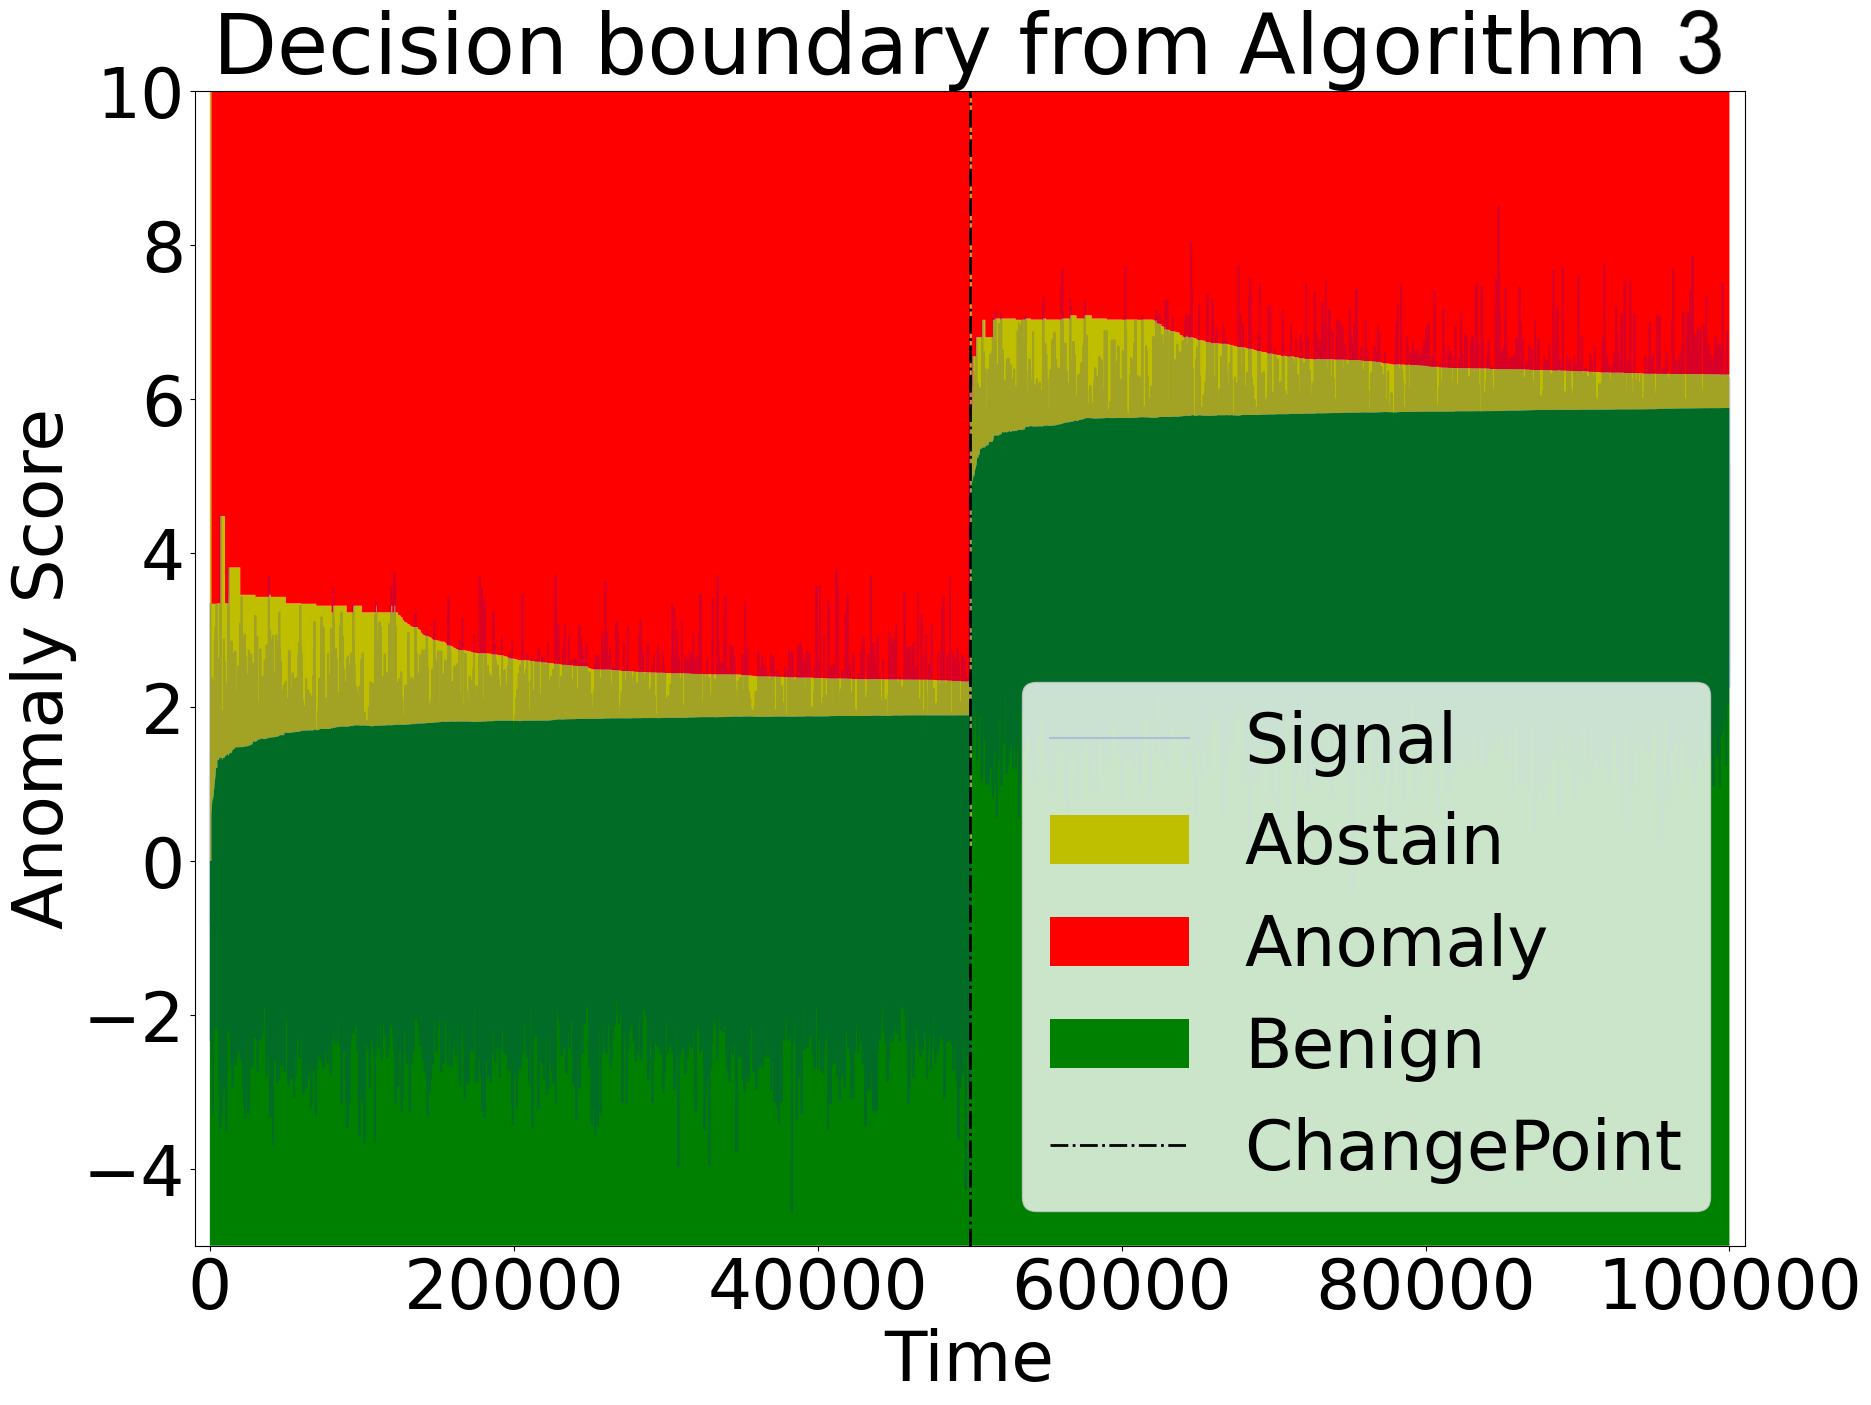
\includegraphics[width=0.55\linewidth]{anomaly/figs/algo_2_example.png}
%     \caption{Algorithm 3 output on a piece-wise stationary stream. \sofi{remake this figure}}
%     \label{fig:s1}
%     \vspace{-1.5em}
% \end{figure}

Going beyond the  i.i.d. case, we consider a piece-wise stationary stream without offline dataset.
Our method in Algorithm \ref{alg:two} uses a change-point detection Algorithm \ref{alg:change_point} from \cite{shekhar2023sequential} as a sub-routine. We need a  definition to state the main result of this section. %Algorithm \ref{alg:change_point} is the forward-backward CS strategy from \cite{shekhar2023sequential}, where a change-point is detected at time $t$, if there exists $1 \leq \tau < t$ with $C(p,\alpha,S_{1:\tau})$ and $C(p,\alpha,S_{\tau+1:t-1})$ having an empty intersection.
% We set additional notation to describe the algorithm. Given the data-stream $(S_t)_{t \geq 1}$ and $t_1 < t_2$ integers, define the set $C(p,\alpha,S_{t_1:t_2})\subseteq \mathbb{R}$ as 
%     \begin{multline}
%         C(p, \alpha, S_{t_1:t_2}) = \bigg[ \widehat{Q}(p-u_{t_2-t_1+1}(\alpha); S_{t_1:t_2}), \\  \widehat{Q}(p+u_{t_2-t_1+1}(\alpha); S_{t_1:t_2}) \bigg].
%         \label{eqn:modified_cs}
%    \end{multline}
% The definition in Equation (\ref{eqn:modified_cs}) is a generalization of the definition in Equation (\ref{eq:cs}) that changes the starting index from $1$ to $t_1$.
%Algorithm \ref{alg:two} detects a change at time $t$, if there exists $1 \leq \tau < t$ such that $C(p,\alpha,S_{1:\tau})$ and $C(p,\alpha,S_{\tau+1:t})$ are non-intersecting, 
%When a change is detected, Algorithm \ref{alg:two} restarts the stationary algorithm. %The full pseudo-code is given in Algorithm \ref{alg:two}. 
%process, a common framework as seen in \cite{sankararaman2023online}.

% \begin{definition}(Piece-wise stationary process) Let $T$ be the time horizon and let $H_T < T$ be the total number of change points. Define a set of strictly increasing time indices  $1 < \tau_1 < \tau_2 \cdots < \tau_{H_T}$ as change points; let $\tau_0 = 0$ and $ \tau_{H_T+1} = T$. The process, $S_1, \cdots, S_T$ is  identified by the quadruple $\Bigl(T,H_T, (\tau_c)_{c=0}^{H_T}, (f_c)_{c=0}^{H_T}\Bigr)$, such that $\forall k \in [1, H_T]$:
% \begin{itemize}[noitemsep,topsep=-3pt,labelwidth=!, labelindent=0pt]
%    \item $\forall t \in [\tau_k,\tau_{k+1})$, $S_t \sim f_k$ i.i.d., with the $p$-quantile of distribution $f_k$ denoted as $ Q_k$
%     \item  $Q_k \neq Q_{k+1}$
% \end{itemize}
% \label{def:piecewise}
% \end{definition}

% \begin{figure}[h!]
%     \centering
%     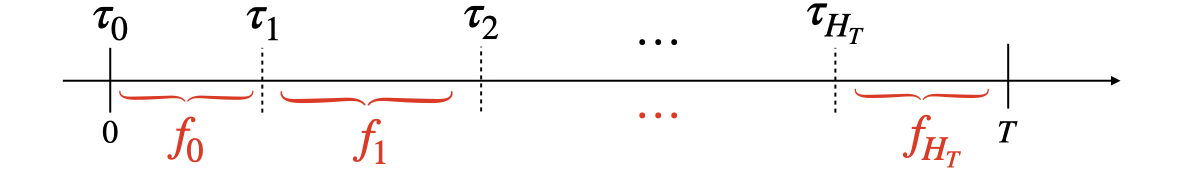
\includegraphics[width=0.9\linewidth]{anomaly/figs/piecewise.jpeg}
%     \caption{The piece-wise stationary process}
%     \label{fig:enter-label}
%     \vspace{-0.8em}
% \end{figure}
 % The anytime-valid property of CSs allows us to bound detection delay and probability of mis-detection, as we show in the following analysis. 


\subsection{Measure of distribution shift}

%We assume all of the distributions in our online stream is \textit{unknown}. In this setting, it is crucial to relate the magnitude of changes (e.g. in our case the shift of quantiles) to the number of available observations between changes \cite{maillard2019sequential}. We therefore introduce some assumptions.

%We define a measure of distribution shift, which dictates the complexity of non-stationarity detection.
%The following is the main definition of distribution shift.

\begin{definition}[quantile shift]
For two continuous distributions $f,g$  on $\mathbb{R}$ with quantile functions  $Q_f(\cdot), Q_g(\cdot) : [0,1] \to \mathbb{R}$ respectively, the distance at quantile $p \in (0,1)$ denoted as $\text{Shift}(f,g,p)$ is defined as
% \begin{multline*}
%     \text{Shift}(f,g,p) := \sup \bigg\{ \Delta \geq 0: \max\bigg[Q_f\left(p-\frac{\Delta}{2}\right) - \\ Q_g\left(p + \frac{\Delta}{2}\right) ,  Q_g\left(p-\frac{\Delta}{2}\right) - Q_f\left(p + \frac{\Delta}{2}\right) \bigg] \geq 0 \bigg\}.
%     \end{multline*}

\begin{multline*}
    \text{Shift}(f,g,p) := \sup \{ \Delta \geq 0: \max[Q_f\left(p-{\Delta}\right) -  Q_g\left(p + {\Delta}\right) ,  Q_g\left(p-{\Delta}\right) - Q_f\left(p + {\Delta}\right) ] \geq 0 \}.
    \end{multline*}
\label{def:quantile_shift}
\end{definition}

Observe that for any two continuous distributions $f$ and $g$, $\text{Shift}(f,g,p) \in [0,1]$ and $\text{Shift}(f,g,p) = 0$ if and only if $f$ and $g$ have identical $p$th quantile. %In words, this definition states that a distribution shift occurs at time $t \geq 2$ if and only if the $p$th quantile at time $t-1$ is different from that at time $t$. 
The following proposition shows that the quantile shift is the non-stationary measure that governs the delay in detecting a change-point.

%We will show in Theorem \ref{thm:online_shift} that the number of FP, FN and abstain guarantees scale this magnitude of distribution shift. %In that regard, Definition \ref{def:quantile_shift} is the most genera; definition since time $t$ is not considered a change point, and thus does not impact performance guarantees, if the distribution at time $t-1$ and $t$ are different, but having identical $p$th quantile.
% %



\begin{algorithm}
\caption{Change detection \cite{shekhar2023sequential}}\label{alg:change_point}
\SetKwInOut{Input}{Input}
\SetKwInOut{Output}{Output}
\Input{$p, \alpha \in (0,1)$, sequence $S_{1:n}$ }
\Output{Binary variable if input has a change-point}

$\widetilde{C} \gets \bigcap_{s \leq n}C(p, \alpha, S_{1:s})$ $\forall t \in [n]$\;

$\widehat{C} \gets \bigcap_{s \leq n}C(p, \alpha, S_{s:n})$ $\forall t \in [n]$\;

\Return $\mathbf{1}( \widetilde{C} \bigcap \widehat{C} = \emptyset)$\: \tcp{1 is a change-point}


\end{algorithm}
 

\begin{algorithm}
\caption{Thresholding without offline data}\label{alg:two}
\SetKwInOut{Input}{Input}
\SetKwInOut{Output}{Output}
\Input{Quantile $p \in (0,1)$, Confidence $\alpha \in (0,1)$}
\Output{Anomaly labels $\hat{y}_1, \hat{y}_2, \ldots$}
$\tau \gets 0$ \tcp*{\small{previous change point}}
\For{  $\text{each time }t \geq 1$ } {
    Receive $t^{th}$ input $S_t$\;
    
    % $\text{forward-CS} \gets CS(\{S_{\tau}, S_{\tau+1}, \ldots, S_t \})$  \;
    
    % $\text{backward-CS} \gets CS(\{ S_t,S_{t-1}, \ldots, S_{\tau} \})$  \;
    
    \uIf{ \text{{\ttfamily Algorithm-}} \ref{alg:change_point} $(p,\alpha,S_{\tau+1:t-1})==1$ }{
    
        $\hat{y}_t \gets * $ \;     \tcp{\small{Change-point detected}}
        
        $\tau \gets t-1$ \;
    }
    \Else{
        $\hat{y}_t \gets$ {{\ttfamily Algorithm-}}\ref{alg:marginal_decision} $(S_t, C(p,\alpha,S_{\tau+1:t-1}))$\;
  }
}
\end{algorithm}


%{\color{red} ---- AS edited till here.}

% \subsection{Good events for quantile estimation}

% \begin{definition}[Good event 2] 
% Let $(S_t)_{t=1}^T \sim \Bigl(T,H_T, (\tau_c)_{c=0}^{H_T}, (f^{(c)})_{c=0}^{H_T}\Bigr)$, with quantile functions of the $H_T+1$ segments given by $(Q^{(c)}(\cdot))_{c=0}^{H_T}$. Define $\gE_2$ as
% \begin{align}
%     \gE_2 := \bigcap_{k=1}^{H_T} \gE_2^{(k)},
%     \label{eqn:good_event_2_defn}
% \end{align}
% where for each $k \in [H_T]$, 
% \begin{multline*}
%         \mathcal{E}_2^{(k)} =  \bigcap_{p \in [0,1]} \bigcap_{t_1 = \tau_{k}}^{\tau_{k+1}} \bigcap_{t_2 = t_1 +1}^{\tau_{k+1}}   \bigg\{ \widehat{Q}(p-u_{t_2 - t_1}(\alpha), S_{t_1:t_2}) \\ \leq Q^{(k)}(p) \leq \widehat{Q}(p-u_{t_2 - t_1}(\alpha), S_{t_1:t_2}) \bigg\},
% \end{multline*}
% where $\widehat{Q}$ is the empirical quantile and $u_{(\cdot)}(\cdot)$ is defined in Equation (\ref{eqn:defn_confidence_width_ut}).
% \label{as:goodevent2}
% \end{definition}
% %\vspace{-1em}
% %
% In words,  $\gE_2$ is the intersection over all the $H_T+1$ stationary segments, where for each segment the quantile estimate is close to the true quantile for all quantiles. Following Corollary $2$ of \cite{howard2022sequential} and an union bound, we get the following.

% \begin{proposition}
%     \begin{align*}
%         \mathbb{P}[\gE_2] \geq 1 - T\alpha.
%     \end{align*}
%     \label{prop:good_event_2_prob}
% \end{proposition}

% \subsection{Change-point detection delay bounds}

% \begin{proposition}[Stream with a single change-point]
% Let $(S_t)_{t=1}^T$ be a piecewise stationary stream with a single change-point, i.e., $H_T = 1$ with the change-point instant $\tau_1 = \tau \in [T]$. Denote by $\Delta := \text{Shift}(f^{(0)}, f^{(1)}, p)$ as the distribution shift magnitude. Denote by $\tau' \in \mathbb{N}$ as the first time when the {\ttfamily if} statement in Algorithm \ref{alg:two} evaluates to {\ttfamily True}, i.e., a change is detected for the first time by Algorithm \ref{alg:two}. Then, under the good event  $\gE_2$  (Definition \ref{as:goodevent2}), 
% \begin{align*}
%     \tau \leq \tau' 
%     &\leq \lceil \inf_{\widetilde{\tau}} \{  u_{\tau}(\alpha) + u_{\widetilde{\tau}-\tau}(\alpha) \leq \Delta \} \rceil,
% \end{align*}
% where $u_t(\alpha)$ is given in Equation (\ref{eqn:defn_confidence_width_ut}). 
% \label{prop:dist_changes}
% \end{proposition}

%This proposition leads to the following simple corollary. %giving a closed form upper bound on the detection delay. 

\begin{proposition}[Stream with a single change-point]
Let $(S_t)_{t=1}^T$ be a piece-wise stationary with one change-point ($H_T = 1$) and quntile shift $\Delta := \text{Shift}(f^{(0)}, f^{(1)}, p) > 0$, at time $\tau_1 = \tau \geq \frac{80}{\Delta^2}\ln \left( \frac{1612}{\alpha \Delta^2}\right)$. Denote by $\tau' \in \mathbb{N}$ as the first time when Algorithm \ref{alg:two} detects a change, i.e., the {\ttfamily if} statement evaluates to {\ttfamily True}. Then, with probability at-least $1-\alpha T$, $ \tau \leq \tau' \leq \tau + \frac{80}{\Delta^2}\ln \left( \frac{1612}{\alpha \Delta^2}\right)$ .
\label{prop:delay_bound}
\end{proposition}

Thus, if there are sufficient pre-change samples, then the change is detected with delay scaling with $\Delta^{-2}$, which is minimax optimal \cite{maillard2019sequential, JMLR:v23:20-1384, shekhar2023sequential}.
As notation, we define detection delay as $D(\cdot, \cdot): [0,1]\times [0,1] \to \mathbb{R}_{+}$ as 
\vspace{-0.1em}
\begin{align}
    D(\Delta,\alpha) := \frac{80}{\Delta^2}\ln \left( \frac{1612}{\alpha \Delta^2}\right). \label{eq:delay_shorthand} 
\end{align}
\vspace{-1.5em}

\subsection{Mistake and abstain bounds}

To give bounds on performance, we make a simplifying assumption that change-points are sufficiently far apart. We refer the readers to Figure \ref{fig:separated_datasets_example} in the appendix for an illustration of the definitions of Assumption \ref{asumption_detectable} and \ref{defn:offline_datasets}.

\begin{assumption}[$\alpha$-detectable]
For a given $\alpha \in (0,1)$, the piece-wise stationary data-stream $(S_t)_{t=1}^T \sim \Bigl(T,H_T, (\tau_c)_{c=0}^{H_T}, (f^{(c)})_{c=0}^{H_T}\Bigr)$ is said to be $\alpha$-detectable if 
% 
\vspace{-0.5em}
\begin{equation*}
    \tau_{k} - \tau_{k-1} \geq \begin{cases}
        D(\Delta_1,\alpha), &k = 1,\\
        D(\Delta_{k-1},\alpha) + D(\Delta_{k},\alpha), &2\leq k\leq H_T\\
        D(\Delta_{H_T}, \alpha), &k=H_T+1
    \end{cases}
\end{equation*}
%     \begin{align*}
%     \tau_{k} - \tau_{k-1} \geq  D(\Delta_{k-1},\alpha) + D(\Delta_{k},\alpha),
% \end{align*}
% and 
% \begin{align*}
%     \tau_1 \geq D(\Delta_1, \alpha),
% \end{align*}
% and
% \begin{align*}
%    T -  \tau_{H_T} \geq D(\Delta_{H_T}, \alpha),
% \end{align*}
holds, where $\Delta_{k} = \text{Shift} (f^{(k)},f^{(k-1)},p)$.%  is the quantile shift for all $k \in [H_T]$ given in Definition (\ref{def:quantile_shift}) and $D(\cdot,\cdot)$ is defined in Equation (\ref{eq:delay_shorthand}).
\label{asumption_detectable}
\end{assumption}

% Assumption \ref{asumption_detectable} implies that change-points are sufficiently far apart. 
 %We show in Lemma \ref{lem:bdd_delay_change_induction} that under this assumption, all change points are detected Algorithm \ref{alg:two}. 

 This assumption is standard to give guarantees for online algorithms with multiple change points on the stream \cite{JMLR:v23:20-1384, sankararaman2023online, cao2019nearly, liu2018change}. Assumption \ref{asumption_detectable} is made for mathematical tractability and is not assumed in experiments. Analysis without Assumption \ref{asumption_detectable} is an open problem (Section $7$ \cite{JMLR:v23:20-1384}). The main result in this section is Theorem \ref{thm:online_shift}.

% \begin{proposition}[Change-point false positives]
%     Let $(S_t)_{t = 1}^T$ be generated from a piece-wise stationary process satisfying Assumption \ref{asumption_detectable} for $\alpha \in (0,1)$. Then, under the good event $\gE_2$, between any two successive detected change-points in Algorithm \ref{alg:change_point}, there exists exactly one true change-point. 
%     \label{prop:cp_fp}
% \end{proposition}

% Proposition \ref{prop:cp_fp} in conjunction with Corollary \ref{prop:delay_bound} gives that under Assumption \ref{asumption_detectable}, if the good event $\gE_2$ holds, then an instance of the stationary algorithm is re-started within a given delay of a true change occurring. This leads to the following performance guarantee on Algorithm \ref{alg:change_point}. 

% {\color{blue}
% \begin{lemma}[Detectability]  If the good event $\mathcal{E}_2$ holds, then the detection delay for a quantile shift of magnitude $\Delta_{(k)}$ is bounded by
% \begin{align}
%     D(\Delta_{(k)},\alpha) = \frac{20}{\Delta_{(k)}^2}\ln \left( \frac{1612}{\alpha \Delta_{(k)}^2}\right). \label{eq:delay_shorthand} 
% \end{align}
% \label{lem:delay}
% \end{lemma}

% \begin{assumption}[All changes are detectable]
% We will assume that the time-interval between change-points are sufficiently far away. Formally, we will assume that for all change-points $1 \leq k \leq H_T$,  
% \begin{align*}
%     \tau_{k} - \tau_{k-1} \geq \max \left( D(\Delta_{k-1},\alpha) , D(\Delta_{k},\alpha) \right)
% \end{align*}
% where for brevity we denote $\Delta_{k} = Shift (f_{k},f_{k+1})$ as defined in definition \ref{def:quantile_shift}.
% \label{as:changes_detectable}
% \end{assumption}
% }

\begin{theorem}[\textbf{main result for Algorithm \ref{alg:two}}]
Let $(S_t)_{t = 1}^T \sim \Bigl(T,H_T, (\tau_c)_{c=0}^{H_T}, (f_c)_{c=0}^{H_T}\Bigr)$ be  a piece-wise stationary data-stream satisfying Assumption \ref{asumption_detectable} for $\alpha \in (0,1)$. Then, with probability at-least $1-2\alpha T$,  Algorithm \ref{alg:two} satisfies {\em both} 
%{\em (i)} $\text{FP} + \text{FN}  \leq \sum_{k=1}^{H_T}D(\Delta_{k},\alpha)$, and {\em (ii)} Number of abstains $ \leq \sum_{k=1}^{H_T} \Bigl[ 7 \sqrt{(\tau_k-\tau_{k-1}) \ln \left( \frac{1612}{\alpha^2} \ln(3(\tau_k-\tau_{k-1})) \right)}  + D(\Delta_{k},\alpha) \Bigr]$,
\begin{itemize}
    \item   $\text{FP} + \text{FN}  \leq \sum_{k=1}^{H_T}D(\Delta_{k},\alpha)$ %$ = H_T \cdot {\gO}(\frac{1}{(\min_k\Delta_{k})^2}) $\footnote{$\mathcal{O}(\cdot)$ ignores constants and poly-log terms in $\frac{T}{\alpha}$.}
    \item abstains $\leq
     \sum_{k=1}^{H_T} \Bigl[ 4 \sqrt{(\tau_k-\tau_{k-1}) \ln \left( \frac{1612}{\alpha^2} \ln(3(\tau_k-\tau_{k-1})) \right)} + D(\Delta_{k},\alpha) \Bigr]$
\end{itemize}
where for all $k \in [H_T]$, $\Delta_{k} = \text{Shift} (f^{(k)},f^{(k-1)},p)$  is the quantile shift defined in Definition (\ref{def:quantile_shift}) and $D(\cdot,\cdot)$ is defined in Equation (\ref{eq:delay_shorthand}).
\label{thm:online_shift}
\end{theorem}



\begin{remark}
    This result shows that $\text{FP}+\text{FN} =  H_T \cdot {\gO}(\frac{1}{(\min_k\Delta_{k})^2}) $\footnote{$\mathcal{O}(\cdot)$ ignores constants and poly-log terms in $\frac{T}{\alpha}$.},  scales only with the number of changes $H_T$, and  abstains at-most $O(\sqrt{H_TT})$ \footnote{Bound follows from Cauchy-Schwartz inequality that $\sqrt{x} + \sqrt{y} \leq \sqrt{2(x+y)}$, $\forall x,y \geq 0$.}. Thus, desiderata $3$ from Section \ref{sec:desiderata} is achieved.  %The bound on abstains 
\end{remark}

{\color{black}
\begin{remark}
      The bound in Theorem \ref{thm:online_shift} holds with probability $1-2\alpha T$. If $(S_t)_{t=1}^T$ is $\alpha/T$-detectable according to Assumption \ref{asumption_detectable}, and with knowledge of $T$, then Algorithm \ref{alg:two} run with input $\alpha/T$ instead of $\alpha$ yields the same order-wise guarantees as Theorem \ref{thm:online_shift} holding with probability $1-2\alpha$. Corollary \ref{cor:weaker_assumption} in the Appendix shows that assuming $(S_t)_{t=1}^T$ being $\alpha/T$ detectable is only weaker by a logarithmic factor compared to the assumption of $\alpha$-detectable.
\end{remark}

% \begin{corollary}
%     For a given $\alpha \in (0,1)$, $T \in \mathbb{N}$, $H_T \leq T-1$ and distributions $(f^{(c)})_{c=0}^{H_T}$, if $\Bigl(T,H_T, (\tau_c)_{c=0}^{H_T}, (f^{(c)})_{c=0}^{H_T}\Bigr)$ is $\alpha$-detectable according to Assumption \ref{asumption_detectable}, then the process $\Bigl( T\lceil  \log(T) \rceil ,H_T, (\tau_c \lceil \log(T) \rceil)_{c=0}^{H_T}, (f^{(c)})_{c=0}^{H_T}\Bigr)$ is $\alpha/T$-detectable.
%     \label{cor:weaker_assumption}
% \end{corollary}

}

\textbf{Proof sketch of Theorem \ref{thm:online_shift}} The crux is an induction argument, that under Assumption \ref{asumption_detectable}, there exists exactly one true change-point between any two successive detected change-points in Algorithm \ref{alg:change_point}. This is formalized in Lemma \ref{lem:bdd_delay_change_induction} in the Appendix. Lemma \ref{lem:bdd_delay_change_induction} along with Proposition \ref{prop:delay_bound} applied recursively to all change-points allows us to decompose the mistakes and abstains over the stationary segments.


%\abishek{Add flex of how this result is proved and in particular, how this is a step up compared to prior results on change-point detection.}






\section{Special Case III: Stationary stream with offline data}

\label{sec:setting_3}

% \begin{algorithm}[h!]
% \caption{OAD with offline datasets}\label{alg:four}
% \SetKwInOut{Input}{Input}
% \SetKwInOut{Output}{Output}
% \Input{Quantile $q$, Confidence $1-\alpha$, offline datasets $\gD_1, \gD_2, \ldots, \gD_L$. }
% \Output{Anomaly labels $\hat{y}_1, \hat{y}_2, \ldots$}
% \For{$j = 1, \ldots, k$}{
%         $CS_{j\text{data}} \gets CS(\gD_j)$\;
%         }
% \For{ $\text{each time }t \geq 1$ } {
%     Receive $t^{th}$ input $S_t$\;
%     $CS_{\text{online}} \gets CS(\{S_i\}_{i=1}^{t})$\;
%     \For{$j = 1, \ldots, k$}{
%         $\text{shift}_j \gets \mathbf{1}(CS_{j\text{data}} \cap CS_{\text{online}} = \emptyset)$\;
%     }
%     \tcp{\small{\# of datasets with CS matching online}}
%     m = $\Sigma_j \mathbf{1}(\text{change}_j = 0)$ \;
%     \uIf{$m =1 $}{
%          \tcp{\small{leverage the matched dataset}}
%         $\hat{y}_t \gets $ Algorithm-\ref{alg:one} $(q, 1-\alpha, \gD_{j\text{match}}  \cup \{S_1,  \ldots , S_t\})$ \;
%     }
%     \Else{
%          \tcp{\small{use online estimation}}
%         $\hat{y}_t \gets$ Algorithm-\ref{alg:one} $(q, 1-\alpha, \{S_1,  \ldots , S_t\})$\;
%   }
% }
% \end{algorithm}

In this section, we return to $(S_t)_{t\geq 1}$ being i.i.d., but give guarantees when the algorithm has access to offline datasets. Our results are based on an \emph{offline} version of Assumption \ref{asumption_detectable} that we state below.

% \begin{definition}[Well separated offline dataset]
% A collection of datasets $\gD_1, \ldots, \gD_L$ are well separated given $p, \alpha$ when their respective confidence sequences do not intersect. i.e. $CS(\gD_i) \cap CS(\gD_j) = \emptyset$ for any $i, k \in [1, L], i\neq j$.
% \label{defn:offline_datasets}
% \end{definition}



\begin{assumption}[\textbf{Well separated offline dataset}]
For $p, \alpha \in (0,1)$, the offline dataset $\gD = \{\{X_l^{(j)}\}_{l=1}^{N_j} \}_{j=1}^K$ is $(p, \alpha)$-separated  with resepct to a piece-wise stationary stream $\Bigl(T,H_T, (\tau_c)_{c=0}^{H_T}, (f^{(c)})_{c=0}^{H_T}\Bigr)$ if both: {\em (i)} for all $i \neq j \in [K]$, $3(u_{N_i}(\alpha) + u_{N_j}(\alpha)) < \text{Shift}(f_{(i)}, f_{(j)}, p)$, and {\em(ii)} for all $j \in [K]$ and stationary-segments $k \in [H_T]$, either $Q^{(k)}(p) = Q_{(j)}(p)$, or  $3u_{N_j}(\alpha) < \text{Shift}(f^{(k)}, f_{(j)},p)$.
\label{defn:offline_datasets}
\end{assumption}
{\color{black} Roughly, a well-separated offline dataset are those that have a sufficient number of samples so as to be distinguishable. Schematic illustrations in Section \ref{sec:illustrations} in the Appendix.} %This assumption is the \emph{offline} version of Assumption \ref{asumption_detectable}. }

% \begin{definition}
%     For every $k \in [K]$, we denote by $Q_{(k)}(p) \in \mathbb{R}$ as the $p$th quantile of the $k$th dataset $\mathcal{D}_k := \{X_l^{(k)}\}_{l=1}^{N_k}$.
%     \label{def:offline_quantile}
% \end{definition}

% \begin{definition}[Good event 3] Define the event $\gE_3$ as 
% \begin{multline}
%     \gE_3 := \bigcap_{k=1}^{K}\bigg\{ Q_{(k)}(p) \in C(p,\alpha, \{X_j^{(k)}\}_{j=1}^{N_k}) \bigg\}  \\ \bigcap_{t \geq 1} \bigg\{ Q(p) \in C(p,\alpha, S_{1:t} \}) \bigg\},
%     \label{eqn:good_event_3}
% \end{multline}
% where $Q(p)$ is the $p$th quantile of the i.i.d. sequence $(S_t)_{t \geq 1}$. 
% \end{definition}





% \begin{algorithm}[h!]
% \caption{Stationary stream with offline datasets}\label{alg:four}
% \SetKwInOut{Input}{Input}
% \SetKwInOut{Output}{Output}
% \Input{Quantile $q$, Confidence $1-\alpha$, offline datasets $\gD_1, \gD_2, \ldots, \gD_K$. }
% \Output{Anomaly labels $\hat{y}_1, \hat{y}_2, \ldots$}
% % \For{$j = 1, \ldots, k$}{
% %         $CS_{j\text{data}} \gets C(p, \alpha, \gD_j)$\;
% %         }
% \For{ $\text{each time }t \geq 1$ } {
%     Receive $t^{th}$ input $S_t$\;
    
%     % $CS_{t}^{(\text{online})} \gets C(p, \alpha,S_{1:t})$\;
    
%     $J_{\text{match}} \gets  \{ j : C(p, \alpha, \gD_j)\cap C(p, \alpha,S_{1:t}) \neq \emptyset \}$\;
    
%     \uIf{$|J_{\text{match}}| =1 $}{
%     %$j_{\text{match}} \gets \sup \{ j : C(p, \alpha, \gD_j)\cap C(p, \alpha,S_{1:t}) \neq \emptyset \}$\;
    
%         $\hat{y}_t \gets $  \small{Algo-\ref{alg:marginal_decision} $(S_t, C(p,\alpha, \gD_{J_{\text{match}}}  \cup \{S_{\tau:t}))$}\; \tcp{\small{use online and offline dataset}}
%     }
%     \Else{
       
%         $\hat{y}_t \gets$ \small{Algo-\ref{alg:marginal_decision} $(S_t, C(p,\alpha,  \{S_{\tau:t}))$}\;  \tcp{\small{use online data only}} %\small{Algo-\ref{alg:one} $(p, 1-\alpha, \{S_{\tau},  \ldots , S_t\})$}\;
%   }
% }
% \end{algorithm}
% In words, $\gE_3$ is the intersection of good event $\gE_1$ in equation \ref{eqn:good_event_defn} for the online stream, and all of the $K$ offline dataset streams. A simple union bound over the $K+1$ streams gives that the good-event $\mathbb{P}[\gE_3]\geq 1-(K+1)\alpha$. 
The main result of this section is how to make decision at time $t$ which is summarized in Algorithm \ref{alg:decision_making_datasets}. In a nutshell, Algorithm \ref{alg:decision_making_datasets} uses the offline dataset if and only if there exists \emph{exactly one} of the $K$ offline dataset whose CS intersects the CS constructed from $S_{1:t}$. The decision at time $t$ is made by constructing a with the unique offline dataset (if it exists) and the online stream using Algorithm \ref{alg:marginal_decision}.


\begin{algorithm}
\caption{Decision making with offline data}\label{alg:decision_making_datasets}
\SetKwInOut{Input}{Input}
\SetKwInOut{Output}{Output}
\Input{$p,\alpha \in (0,1)$, Online data $S_{1}, \ldots, S_n$, offline datasets $\gD_{1}, \ldots, \gD_K$. }
\Output{Anomaly label $\hat{y} \in \{0,1,*\}$}
% \For{$j = 1, \ldots, k$}{
%         $CS_{j\text{data}} \gets C(p, \alpha, \gD_j)$\;
%         }
    % $CS_{t}^{(\text{online})} \gets C(p, \alpha,S_{1:t})$\;
    
    $J_{\text{match}} \gets  \{ j : C(p, \alpha, \gD_j)\cap C(p, \alpha,S_{1:n-1}) \neq \emptyset \}$\;
    
    \uIf{$|J_{\text{match}}| =1 $}{
    %$j_{\text{match}} \gets \sup \{ j : C(p, \alpha, \gD_j)\cap C(p, \alpha,S_{1:t}) \neq \emptyset \}$\;
    
        $\hat{y} \gets $  \small{{{\ttfamily Algorithm-}}\ref{alg:marginal_decision}  $(S_n, C(p,\alpha, \gD_{J_{\text{match}}}  \cup \{S_{1:n-1}))$}\; \tcp{\small{use online and offline dataset}}
    }
    \Else{
       
        $\hat{y} \gets$ \small{{{\ttfamily Algorithm-}}\ref{alg:marginal_decision}  $(S_n, C(p,\alpha,  \{S_{1:n-1}))$}\;  \tcp{\small{use online data only}} %\small{Algo-\ref{alg:one} $(p, 1-\alpha, \{S_{\tau},  \ldots , S_t\})$}\;
  }
  \Return $\hat{y}$\;
\end{algorithm}

We set some more notation to state the result.
For all $j \in [K]$, $\widehat{\tau}_j = \inf \{ \widehat{\tau}: 3(u_{\widehat{\tau}}(\alpha) + u_{N_j}(\alpha)) \leq \text{Shift}(f,f_{(j)},p) \},$
where $\widehat{\tau}_j = +\infty$ if $\text{Shift}(f,f_{(j)},p)=0$. Assumption \ref{defn:offline_datasets} guarantees that if $\text{Shift}(f,f_{(j)},p)>0$, then $\widehat{\tau}_j  < \infty$ is finite independent of $T$.
%Denote by 
\begin{align}
    \widehat{\tau} := \max \{ \lceil \widehat{\tau}_j \rceil : \text{Shift}(f,f_{(j)}, p) > 0 \}.
    \label{eqn:defn_tau_hat}
\end{align}
%The main result of this section is the following.

\begin{theorem}[\textbf{Main result for Algorithm \ref{alg:decision_making_datasets}}] Let the online stream $(S_t)_{t \geq 1} $ be i.i.d. from distribution $f$ and the $j \in [K]$ offline dataset with $N_j$ i.i.d. samples have distribution $f_{(j)}$. Further, let the offline dataset be $(p,\alpha)$ well-separated for some $\alpha \in (0,1)$ (Def. \ref{defn:offline_datasets}). Let $\Delta = \min_{1\leq j \leq K} \text{Shift}(f, f_{(j)},p)$. Then,for all times $T \in \mathbb{N}$, with probability at-least $1-(K+T)\alpha$, if the decision $\hat{y}_t$ is made by Algorithm \ref{alg:decision_making_datasets} with inputs $p, \alpha, S_{1:t}$ and $\mathcal{D}_{1:K}$, we have:
\begin{itemize}[itemsep=2pt,topsep=-1pt,labelwidth=!, labelindent=0pt]
\item  If $\Delta = 0$, then $\text{FP} + \text{FN} = 0$ and Abstains  $\leq {B}(N+T,\alpha) - \frac{B(N,\alpha)}{28} + \widehat{\tau}$, %where  $N = \min \{N_j: \text{Shift}(f,f_{(j)},p)=0\}$, $B(\cdot, \cdot) : \mathbb{N} \times [0,1] \to \mathbb{R}_{+}$ is given by $B(Y,\alpha) =  7\sqrt{Y \ln \left( \frac{1612\ln(3Y)}{\alpha^2} \right)}$ and $\widehat{\tau}$ is defined in Equation (\ref{eqn:defn_tau_hat}).% and  $\widetilde{\Delta} = \min \{ \text{Shift}(f,f_{(j)}, p) : \text{Shift}(f,f_{(j)}, p) > 0 \}$. 
\item If  $\Delta > 0$, then $\text{FP}+\text{FN} \leq \widehat{\tau} $ and Abstains  $ \leq \widehat{\tau} + B(T,\alpha)$,
\end{itemize}
where  $N = \min \{N_j: \text{Shift}(f,f_{(j)},p)=0\}$, $B(\cdot, \cdot) : \mathbb{N} \times [0,1] \to \mathbb{R}_{+}$ is given by $B(Y,\alpha) =  7\sqrt{Y \ln \left( \frac{1612\ln(3Y)}{\alpha^2} \right)}$ and $\widehat{\tau}$ is defined in Equation (\ref{eqn:defn_tau_hat}).
% {\em (i)} If $\Delta = 0$, then $\text{FP} + \text{FN} = 0$ and Abstains   $\leq {B}(N+T,\alpha) - B(N,\alpha)$ where  $N = \min \{N_j: \text{Shift}(f,f^{(j)},p)=0\}$.

% {\em(ii)} Else if  $\Delta > 0$, then $\text{FP}+\text{FN} \leq D(\Delta,\alpha) $ and Abstains  $ \leq D(\Delta,\alpha) + B(T,\alpha)$,

% where $B(\cdot, \cdot) : \mathbb{N} \times [0,1] \to \mathbb{R}_{+}$ is given by $B(Y,\alpha) = 4 \sqrt{Y \ln \left( \frac{1612\ln(3Y)}{\alpha^2} \right)}$. 

% \begin{itemize}[itemsep=2pt,topsep=1pt,labelwidth=!, labelindent=0pt]
%     \item If $\Delta = 0$, let $N:= \min \{N_j: \text{Shift}(f,f^{(j)},p)=0\}$. Then $\text{FP} + \text{FN} = 0$ and Abstains   $\leq 4 \sqrt{(N+T) \ln \left( \frac{1612\ln(3(N+T))}{\alpha^2} \right)}- 4 \sqrt{N \ln \left( \frac{1612\ln(3N)}{\alpha^2} \right)}$.
%     % \begin{itemize}[noitemsep,labelwidth=!, labelindent=0pt]
%     %     \item $FP= 0$, $FN=0$
%     %     \item Abstains $= 4 \sqrt{(N+T) \ln \left( \frac{1612\ln(e(N+T))}{\alpha^2} \right)}- 4 \sqrt{N \ln \left( \frac{1612\ln(eN)}{\alpha^2} \right)}$
%     % \end{itemize}
%     \item Else if  $\Delta > 0$, then $\text{FP}+\text{FN} \leq D(\Delta,\alpha) $ and abstains is at-most $ D(\Delta,\alpha) + 4 \sqrt{T \ln \left( \frac{1612\ln(3T)}{\alpha^2} \right)}$.
%     % \begin{itemize}[noitemsep,labelwidth=!, labelindent=0pt]
%     %     \item $FP+FN \leq D(\Delta,\alpha) $
%     %     \item Abstains $\leq D(\Delta,\alpha) + 4 \sqrt{T \ln \left( \frac{1612\ln(eT)}{\alpha^2} \right)}$
%     % \end{itemize}
% \end{itemize}
\label{thm:setting_3}
\end{theorem}

We now read off several remarks from this result. 

\textbf{Improved performance if offline dataset is useful.} The case of $\Delta=0$ implies that the online stream's $p$th quantile equals at-least one of the $K$ offline dataset's $p$th quantile, i.e., the offline dataset is useful. In this case, Theorem \ref{thm:setting_3} guarantees $0$ FP and FN, and  abstains at-most $\gO(\sqrt{N+T} - \sqrt{N})$, which is much smaller compared to the $\gO(\sqrt{T})$ bound from Algorithm \ref{alg:one} without offline data.


\textbf{Bounded degradation if offline dataset is arbitrary.} The case of $\Delta > 0$  implies that the online stream's $p$th quantile does not match any of the $K$ offline dataset's $p$th quantile, i.e., the offline dataset is useless. In this case, Theorem \ref{thm:setting_3}, guarantees FP $+$ FN $\leq \widehat{\tau}$ and abstains $\leq \gO(\sqrt{T}) + \widehat{\tau}$. Thus performance compared to Theorem \ref{the:iid} is worse \emph{only by an additive term independent of the stream length $T$}, thereby achieving desiderata $4$ from Section \ref{sec:desiderata}.
 Equation (\ref{eq:delay_shorthand}) implies that $\widehat{\tau}$ is a {sample complexity upper bound} to confidently reject the hypothesis that one of the $K$ offline dataset's  $p$th quantile equals that of $f$.%of $(S_t)_{t \geq 1}$ and one of the offline dataset are identical. %determining an offline dataset to be irrelevant since from the Def. in Equation (\ref{eq:delay_shorthand}), $D(\Delta, \alpha)$ is an upper bound on the number of samples of the online stream needed 

%This term $D(\Delta, \alpha)$ is larger when the \emph{complexity} of distinguishing the online stream from the offline dataset is harder and is the \emph{penalty} incurred  when the offline datasets are not reflective of the online distribution. 
  Thus, Algorithm \ref{alg:decision_making_datasets} adapts to the complexity yielding much lower abstains in the case when the online distribution matches one of the offline dataset, while simultaneously having bounded degradation \emph{in the worst-case}. 

%\subsection{Proof Sketch of Theorem \ref{thm:setting_3}}

% To set the ideas, we will need some definitions. 

% \begin{definition}
%     For every $k \in [K]$, we denote by $Q_{(k)}(p) \in \mathbb{R}$ as the $p$th quantile of the $k$th dataset $\mathcal{D}_k := \{X_l^{(k)}\}_{l=1}^{N_k}$.
%     \label{def:offline_quantile}
% \end{definition}

% \begin{definition}[Good event 3] Define the event $\gE_3$ as 
% \begin{multline}
%     \gE_3 := \bigcap_{k=1}^{K}\bigg\{ Q_{(k)}(p) \in C(p,\alpha, \{X_j^{(k)}\}_{j=1}^{N_k}) \bigg\}  \\ \bigcap_{t \geq 1} \bigg\{ Q(p) \in C(p,\alpha, S_{1:t} \}) \bigg\},
%     \label{eqn:good_event_3}
% \end{multline}
% where $Q(p)$ is the $p$th quantile of the i.i.d. sequence $(S_t)_{t \geq 1}$. 
% \end{definition}

%We outline a good-event in Equation (\ref{eqn:good_event_3}) in which all the different quantiles on the online and offline datasets are estimated correctly. 
\textbf{Proof Sketch.} The crux of the proof is that, if the online stream's quantile matches that of one of the offline dataset, then {\em(i)} for all times, $J_{\text{match}} \geq 1$ in Algorithm \ref{alg:decision_making_datasets}, and {\em(ii)} \emph{ for all times} $t \geq \widehat{\tau}$, $J_{\text{match}} = 1$. Similarly, if no offline dataset's $p$th quantile matches that of the online $p$th quantile, for all times $t \geq \widehat{\tau}$, $J_{\text{match}} = 0$ and thus Algorithm \ref{alg:decision_making_datasets} will only use the online stream's samples for decision making. 

% In words, $\gE_3$ is the intersection of good event $\gE_1$ in equation \ref{eqn:good_event_defn} for the online stream, and all of the $K$ offline dataset streams. A simple union bound over the $K+1$ streams gives that the good-event $\mathbb{P}[\gE_3]\geq 1-(K+1)\alpha$.     The core technical argument in the proof of Theorem \ref{thm:setting_3} is the definition of the good event $\gE_3$ in Equation (\ref{eqn:good_event_3}). 

% First observe that since the offline datasets are disjoint (Definition \ref{defn:offline_datasets}), there can be at-most one offline dataset whose $p$th quantile will match that of the online stream. Under the good event $\gE_3$, \emph{eventually} the online CS will only intersect with this offline CS and thus eventually lead to low number of abstains. However, if the online stream's $p$th quantile does not match any of the offline datasets, then again \emph{eventually} the online CS will not intersect with any offline CS. Thus, in this case, eventually, 


%On the other hand if the online distribution does not match any of the offline distribution,  than the performance is comparable to the setting in which no offline data is present (Theorem \ref{the:iid}).

%\abishek{Add flex of how this result is proved.}



\section{The General Case} %: Piece-wise stationary stream with offline data
\label{sec:general_setting}
%\vspace{-0.5em}
This setting generalizes all the special cases. 
%The pseudo-code is given in Algorithm \ref{alg:five} builds upon the ideas developed for each of the special cases.
%We  require additional notation. 
For each offline dataset $j \in [K]$ and stationary segment of the online stream $k \in [H_T]$, denote by  $\Delta^{(j;k)} = \text{Shift}(f_{(j)}, f^{(k)},p)$, where $f_{(j)}$ is the distribution of offline dataset $j$ and $f^{(k)}$ the distribution of the $k$th online segment (Def. \ref{def:piecewise}). Identical to Theorem \ref{thm:online_shift}, for each $k \in [H_T]$,  $\Delta_k =  \text{Shift} (f^{(k)},f^{(k-1)},p)$ is the shift between the $k$th and $k-1$th online segment. Similar to Theorem \ref{thm:setting_3}, for each $k \in [H_T]$ and offline dataset $j \in [K]$,  $\widehat{\tau}_j^{(k)} = \inf \{ \widehat{\tau}: 3(u_{\widehat{\tau}}(\alpha) + u_{N_j}(\alpha)) \leq \text{Shift}(f^{(k)},f_{(j)},p) \}$, where $\widehat{\tau}_j^{(k)} = \infty$ if $\text{Shift}(f^{(k)},f_{(j)},p)=0$.  Assumption \ref{defn:offline_datasets} guarantees $\text{Shift}(f^{(k)},f_{(j)},p)>0\implies\widehat{\tau}_j^{(k)}  < \infty$. Similar to Eq. (\ref{eqn:defn_tau_hat}),  $\widehat{\tau}^{(k)} = \max \{ \lceil \widehat{\tau}_j^{(k)} \rceil \text{ : } \widehat{\tau}_j^{(k)}  < \infty \}.$
% is finite independent of $T$.%Given a piecewise-stationary stream $(S_t)_{t=1}^T$ and the $K$ offline datasets, for each segment $k \in [H_T]$, denote by 
\begin{equation}
    \widetilde{D}_k(\alpha) = D(\Delta_k,\alpha) + \widehat{\tau}^{(k)}.
    \label{eqn:D_tilde}
\end{equation}

In words, $\widetilde{D}_k(\alpha)$ is the \emph{worst-case} delay after the $k$th change point has occurred on the data-stream for Algorithm \ref{alg:five} to both {\em(i)} detect that the online stream has undergone a shift, and {\em(ii)} identify if any of the offline datasets' $p$th quantile matches the new $p$th quantile. 


\begin{algorithm}[h!]
\caption{General thresholding algorithm}\label{alg:five}
\SetKwInOut{Input}{Input}
\SetKwInOut{Output}{Output}
\Input{ $p, \alpha \in (0,1)$, offline datasets $\gD_1, \gD_2, \ldots, \gD_K$. }
\Output{Anomaly labels $\hat{y}_1, \hat{y}_2, \ldots$}
$\tau \gets 0$  \tcp*{\small{previous change point}}
% \For{$j = 1, \ldots, K$}{
%         $CS_{j\text{forward}} \gets C(p,\alpha,\gD_j)$\;
%         }
\For{ $\text{each time }t \geq 1$ } {
    Receive $t^{th}$ input $S_t$\;
    
    % $CS_{\text{online}} \gets C(p,\alpha, S_{\tau:t})$  \;
    % $CS_{\text{backward}} \gets CS(\{S_i\}_{i=\tau}^{t})$\;
    % \tcp{\small{detect shift}}
    \uIf{{\ttfamily Algorithm-}\ref{alg:change_point} $(p,\alpha,S_{\tau+1:t-1})==1$}{
        $\hat{y}_t \gets * $ \; \tcp{Change-point detected}
        $\tau \gets t-1$ \;
    } \Else {
    $\hat{y}_t \gets \text{{\ttfamily Algorithm-}\ref{alg:decision_making_datasets}} (p,\alpha, S_{\tau+1:t-1}, (\gD_{1:K}))$
  %   \tcp{\small{Check for matching datasets}}
  %   % \For{$j = 1, \ldots, k$}{
  %   %     $\text{m}_j \gets $ \small{$\mathbf{1}(CS_{j\text{forward}-t} \cap CS_{\text{backward}-t} \neq \emptyset)$}\;
  %   % }
  %   m = $\Sigma_j \mathbf{1}(CS_{j\text{forward}-t} \cap CS_{\text{backward}-t} \neq \emptyset)$\;
  %   \uIf{$m =1 $}{
  %       $\hat{y}_t \gets $  \small{Algo-\ref{alg:one} $(p, 1-\alpha, \gD_{j\text{match}}  \cup \{S_{\tau},  \ldots , S_t\})$}\;
  %   }
  %   \Else{
  %       \tcp{\small{use online estimation}}
  %       $\hat{y}_t \gets$  \small{Algo-\ref{alg:one} $(p, 1-\alpha, \{S_{\tau},  \ldots , S_t\})$}\;
  % }
  }
}
\end{algorithm}

% \begin{algorithm}[h!]
% \caption{General thresholding algorithm}\label{alg:five}
% \SetKwInOut{Input}{Input}
% \SetKwInOut{Output}{Output}
% \Input{Quantile $p$, Confidence $1-\alpha$, offline datasets $\gD_1, \gD_2, \ldots, \gD_K$. }
% \Output{Anomaly labels $\hat{y}_1, \hat{y}_2, \ldots$}
% $\tau \gets 0$  \tcp*{\small{previous change point}}
% \For{$j = 1, \ldots, K$}{
%         $CS_{j\text{forward}} \gets C(p,\alpha,\gD_j)$\;
%         }
% \For{ $\text{each time }t \geq 1$ } {
%     Receive $t^{th}$ input $S_t$\;
    
%     $CS_{\text{online}} \gets C(p,\alpha, S_{\tau:t})$  \;
%     $CS_{\text{backward}} \gets CS(\{S_i\}_{i=\tau}^{t})$\;
%     \tcp{\small{detect shift}}
%     \uIf{$CS_{\text{online}-i }\cap CS_{\text{backward}-(t-\tau-i)} = \emptyset$ for any $i \in [1, t-\tau]$}{
%         $\hat{y}_t \gets * $ \;
%         $\tau \gets t$ \;
%     } \Else {
%     \tcp{\small{Check for matching datasets}}
%     % \For{$j = 1, \ldots, k$}{
%     %     $\text{m}_j \gets $ \small{$\mathbf{1}(CS_{j\text{forward}-t} \cap CS_{\text{backward}-t} \neq \emptyset)$}\;
%     % }
%     m = $\Sigma_j \mathbf{1}(CS_{j\text{forward}-t} \cap CS_{\text{backward}-t} \neq \emptyset)$\;
%     \uIf{$m =1 $}{
%         $\hat{y}_t \gets $  \small{Algo-\ref{alg:one} $(p, 1-\alpha, \gD_{j\text{match}}  \cup \{S_{\tau},  \ldots , S_t\})$}\;
%     }
%     \Else{
%         \tcp{\small{use online estimation}}
%         $\hat{y}_t \gets$  \small{Algo-\ref{alg:one} $(p, 1-\alpha, \{S_{\tau},  \ldots , S_t\})$}\;
%   }
%   }
% }
% \end{algorithm}

% To state performance guarantee of Algorithm \ref{alg:five}, we need a definition of a good event, which occurs with high probability.
% \begin{definition}[Good event 4] 
% Given a piece-wise stationary sequence $(S_t)_{t=1}^T := \Bigl(T,H_T, (\tau_c)_{c=0}^{H_T}, (f^{(c)})_{c=0}^{H_T}\Bigr)$, with the quantile functions of the $H_T+1$ different segments given by $(Q^{(c)}(\cdot))_{c=1}^{H_T}$ and $K$ offline datasets that are $(p,\alpha)$ separated according to Definition \ref{defn:offline_datasets}, let
% \begin{align}
% \begin{split}
%     \gE_4 = \underbrace{\bigcap_{l=1}^{K}\bigg\{ Q_{(l)}(p) \in C(p,\alpha, \{X_j^{(l)}\}_{j=1}^{N_l}) \bigg\}}_{\text{Offline dataset's CS contain true quantile}}   \\ \underbrace{\bigcap_{k=0}^{H_T} \bigcap_{t_1 = \tau_{k}}^{\tau_{k+1}} \bigcap_{t_2 = t_1 + 1}^{\tau_{k+1}}   \{ Q^{(k)}(p) \in C(p,\alpha,S_{t_1:t_2}) \}}_{\text{Online stream's CS contain true quantile}},
%         \end{split}
%                 \label{eqn:good_event_4_defn}
% \end{align}
% where the $p$th quantile of the offline datasets $Q_{(l)}(p)$ are defined in Definition \ref{def:offline_quantile}.
% \end{definition}
% \vspace{-0.5em}
% %
% Event $\gE_4$ is the union of $\gE_2$ in equation \ref{eqn:good_event_2_defn} for the online stream along with the event $\gE_3$ in Equation (\ref{eqn:good_event_3}) for the offline datasets. A union bound implies that the event $\mathbb{P}[\gE_4] \geq 1- \alpha (K+T)$. 

%The main result of this paper is stated below.




%The main result of t

\begin{theorem}[\textbf{Main result of Algorithm \ref{alg:five}}] For a desired $\alpha \in (0,1)$, suppose the piece-wise stationary online stream $(S_t)_{t=1}^T \sim \Bigl(T,H_T, (\tau_c)_{c=0}^{H_T}, (f_c)_{c=0}^{H_T}\Bigr)$ is $\alpha$-detectable, i.e., satisfies Assumption \ref{asumption_detectable}, and the offline datasets  $\gD_1, \ldots, \gD_K$ are $(p,\alpha)$-separated according to Definition \ref{defn:offline_datasets}. %Denote by the online quantile shifts as $\Delta_{k} = \text{Shift} (f^{(k)},f^{(k-1)},p)$ for $k \in [H_T]$. 
Then, for all times $T \in \mathbb{N}$, with probability at-least $1-(K+2T)\alpha$,  Algorithm \ref{alg:five} satisfies \emph{both},
%{\em (i)} $\text{FP} + \text{FN}  \leq \sum_{k=1}^{H_T} \widetilde{D}_k(\alpha)$, and {\em(ii)} Abstains $\leq \sum_{k=1}^{H_T} \Bigl[ (1-\mathbf{1}_{\text{Match}_k}) \mathcal{O}(\sqrt{\tau_k - \tau_{k-1}}) \footnote{Constants are in the Appendix and report here the order-wise result to highlight the main terms in the bound. } + \mathbf{1}_{\text{Match}_k}\left(\gO(\sqrt{N^{(k)}+(\tau_k-\tau_{k-1})} - \sqrt{N^{(k)}}) \right) +  \widetilde{D}_k(\alpha) \Bigr]$,
\begin{itemize}
    \item  $\text{FP} + \text{FN}  \leq \sum_{k=1}^{H_T} D(\Delta_k,\alpha) + (1-\mathbf{1}_{\text{Match}_k})\max_{ j \in [K]} \left(\lceil \widehat{\tau}_j^{(k)}\rceil \mathbf{1}_{\text{Shift}(f^{(k)},f_{(j)},p) > 0}\right)$ 
     \item Abstains $ \leq \sum_{k=1}^{H_T} \Bigl[ (1-\mathbf{1}_{\text{Match}_k}) \mathcal{O}(\sqrt{\tau_k - \tau_{k-1}}) \footnote{Constants are in the Appendix and report here the order-wise result to highlight the main terms in the bound. } +  \mathbf{1}_{\text{Match}_k}\left(\gO(\sqrt{N^{(k)}+(\tau_k-\tau_{k-1})} - \sqrt{N^{(k)}}) \right) +  \widetilde{D}_k(\alpha) \Bigr]$
 \end{itemize}
where $\mathbf{1}_{\text{Match}_k} = \mathbf{1}_{Q^{(k)}(p) \in \{Q_{(1)}(p), \cdots, Q_{(K)}(p)\}}$, and $Q^{(k)}(p)$ is the $p$th quantile of the $k$th segment of the online stream (Def. \ref{def:piecewise}), $Q_{(1)}(p), \cdots, Q_{(K)}(p)$ are the $p$th quantiles of the offline datasets (Definition \ref{definition:offline_dataset}),   $N^{(k)} = \min \{N_j: Q_{(j)}(p) = Q^{(k)}(p)\}$ and $\widetilde{D}_k(\alpha)$ is defined in Equation (\ref{eqn:D_tilde}). 
\label{thm:core_theorem}
\end{theorem}

Observe that Theorem \ref{thm:core_theorem} recovers Theorem \ref{thm:setting_3}  if $(S_t)_{t\geq 1}$ is i.i.d. Theorem \ref{thm:core_theorem} shows that even in the general case,  $\text{FP} + \text{FN}$ only scale with the number and complexity of change-points, and not with the stream length $T$. 
%The term $\widetilde{D}_k(\alpha)$ for each $k \in [H_T]$ in Equation (\ref{eqn:D_tilde}) is the delay incurred in both detecting the $k$th change-point and deciding which if any of the offline dataset's $p$th quantile matches the $k$th stationary segment.
% We now read off several remarks from Theorem \ref{thm:core_theorem}.


\begin{figure}
\centering
\begin{subfigure}{.48\columnwidth}
  \centering
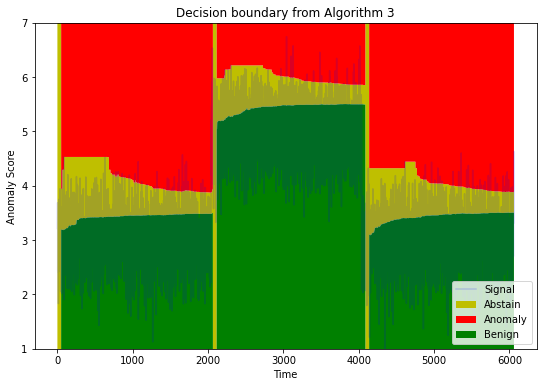
\includegraphics[width=\linewidth]{anomaly/figs/4-2.png}
  %\caption{A subfigure}
  \caption{}
  \label{fig:s41}
\end{subfigure}%
\begin{subfigure}{.48\columnwidth}
  \centering
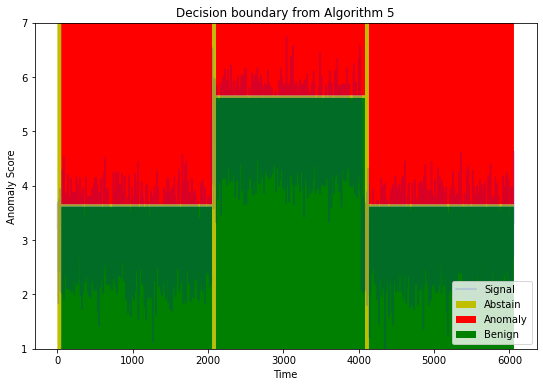
\includegraphics[width=\linewidth]{anomaly/figs/4-1.png}
  %\caption{Anomaly threshold set using a fixed cold-start period}
  \caption{}
  \label{fig:s42}
\end{subfigure}%
\vspace{-0.5em}
\caption{Decision boundaries for the same synthetic data stream, without offline dataset $(a)$ and with $(b)$. Incorporating datasets allows us to significantly reduce abstention.}\vspace{-2em}
\label{fig:s4_example}
\end{figure}
%\vspace{-4em}

%\textbf{Mistakes do not scale with $T$.}
   
% \begin{itemize}
%     \item Case $\Delta = 0$:
%     \begin{itemize}
%         \item $FP= 0$, $FN=0$
%         \item Abstains $= 4 \sqrt{(N+T) \ln \left( \frac{1612\ln(e(N+T))}{\alpha^2} \right)}- 4 \sqrt{N \ln \left( \frac{1612\ln(eN)}{\alpha^2} \right)}$
%     \end{itemize}
%     \item Case  $\Delta > 0$:
%     \begin{itemize}
%         \item $FP+FN \leq D(\Delta,\alpha) $
%         \item Abstains $\leq D(\Delta,\alpha) + 4 \sqrt{T \ln \left( \frac{1612\ln(eT)}{\alpha^2} \right)}$
%     \end{itemize}
% \end{itemize}

%We show in Corollary \ref{cor:general_flex_1} that when the offline datasets when, abstains are reduced (see also Figure \ref{fig:s4_example}).

\textbf{Abstains reduced if offline data is useful.}
     Suppose the online stream $(S_t)_{t=1}^T$  and the offline datasets  $\gD_{1}, \ldots, \gD_K$ are such that for all segments $k \in [H_T]$, there exists an offline dataset $j \in [K]$ s.t. $Q^{(k)}(p) = Q_{(j)}(p)$. Theorem \ref{thm:core_theorem} guarantees that  abstains $\leq \mathcal{O}\left(\sqrt{H_T N} \left(\sqrt{1+\frac{T}{N}} - 1 \right)\right) + \sum_{k=1}^{H_T}\widetilde{D}_k( \alpha)$, where $N = \min \{N_j \text{ : } \exists k \in [H_T] \text{ : } Q_{(j)}(p) = Q^{(k)}(p) \}  $ is size of the smallest useful offline dataset. Thus, if the useful offline data is large ($N >> T$), the fraction of abstains is small even in the presence of non-stationarity (Fig. \ref{fig:s4_example} ). 
     %\label{cor:general_flex_1}
     
%Corollary \ref{cor:general_flex_1} shows that in the worst-case when the offline distribution can be arbitrary, the performance degradation is bounded. 

\textbf{Bounded degradation if offline data is arbitrary.}
Theorem \ref{thm:core_theorem} proves that in the worst-case when the offline datasets are arbitrary, abstains are at-most $ \mathcal{O}(\sqrt{H_T T}) + \sum_{k=1}^{H_T}\widetilde{D}_k(\alpha)$, which is comparable to Theorem \ref{thm:online_shift}, with an additional additive term of $\sum_{k=1}^{H_T}\widetilde{D}_k(\alpha)$. This extra term arises due to incurring delay in both identifying a change-point on the online stream, and deciding that either the new segment has the same $p$th quantile as one of the offline datasets or not. This penalty is incurred since Algorithm \ref{alg:five} does not know both the time of change-points and if the $p$th quantile of any offline datasets equals that of the online. Thus, Theorem \ref{thm:core_theorem} is adaptive, yielding low mistakes and abstains in the event that the offline dataset is useful while simultaneously bounding worst-case performance independent of $T$ and $N$ when the offline dataset is arbitrary. 


     %For a desired $\alpha \in (0,1)$, suppose the online stream $(S_t)_{t=1}^T$ satisfy the conditions in Theorem \ref{thm:core_theorem}  and the offline datasets  $\gD_{1}, \ldots, \gD_K$ satisfy Assumption \ref{as:offline_detectable}, but are otherwise arbitrary. Then, with probability at-least $1- (K+T)\alpha$, 
     %\label{cor:general_flex_2}

%Corollary \ref{cor:general_flex_2} shows that in the worst case when the offline distributions are arbitrary, the number of abstains  %Moreover, the worst case bound is independent of stream length $T$ and offline dataset size $N$. 

% \begin{remark}[Best case scenario for Algorithm \ref{alg:five}] Even though the worst case bounds of Theorem \ref{thm:core_theorem} is the same as that of Theorem \ref{thm:online_shift} (online distribution shift setting), we can apply the analysis of Theorem \ref{thm:setting_3} (stationary + dataset setting) on each stationary piece of the stream. If all of the pieces match the offline datasets, the number of abstains is reduced to be less than $ \sum_{k=1}^{H_t} \left( D(\Delta_k,\alpha) + \gO(\sqrt{N+(\tau_k-\tau_{k-1})} - \sqrt{N})\right) $. 
% \end{remark}




%\abishek{Add flex of how this result is proved.}



\section{Experiments}
%\vspace{-0.8em}
\subsection{Synthetic data experiments}
%\vspace{-0.8em}
We evaluated our algorithm using two synthetic datasets, reflecting all scenarios discussed in this paper. The metrics are abstention percentages (Abs. \%) and mistake counts (FP + FN), averaged over 1000 streams each with 2000 samples drawn from Normal distributions with random parameters, with $p=1-10^{-2}$ and $\alpha=10^{-3}$. Our comparisons against common thresholding baselines: $\tau^{30\%}$ for static thresholding, {\ttfamily DSpot} for dynamic thresholding, and {\ttfamily EQ} for empirical quantiles using online gradient descent, are presented in Table \ref{tab:synthetic}. Implementation details and additional experiments on Pareto distributions are in Appendix \ref{app:exp1}. These results confirm our algorithm's high accuracy, adaptability to distribution shifts, and effective learning from offline data, as outlined in Section 1's desiderata. Figure \ref{fig:synthetic} illustrates how our algorithm's abstention rates and errors grow over time, corroborating our theoretical results.
%theory that (1) our algorithm makes very little FP and FN, and (2) abstains are reduced significantly with the introduction of offline datasets.  evident in the low number of mistakes,
\begin{table}[h!]
    \centering
    \begin{tabular}{cc|c|c |c| c|c}
    \toprule
        shift & data &  & Ours &  $\tau^{30\%}$  & DSpot & EQ \\
        \midrule
        \midrule
         \multirow{2}{*}{x}  & \multirow{2}{*}{x}  &
         Abs. \%& $12.1$ \plusminus{1.4} & $30$ & $15$ & $0$ \\
          && FP+FN & $\mathbf{0}$ \plusminus{0}  & $5.3$ \plusminus{3.7} & $9.1$ \plusminus{3.6} & $3.9$ \plusminus{2.1}  \\
          \midrule
         \multirow{2}{*}{\checkmark}  & \multirow{2}{*}{x}  &  
         Abs. \%& $32.7$ \plusminus{9.1} & $30$ &  $15$ & $0$  \\
        && FP+FN & $\mathbf{5.2}$ \plusminus{1.3} &  $195$  \plusminus{71} & 225 \plusminus{95} & 219 \plusminus{71} \\
                    \midrule
        \multirow{2}{*}{x} & \multirow{2}{*}{\checkmark}  &  
        Abs. \% & 9.3 \plusminus{1.2} & $30$&  $15$ & $0$ \\
          && FP+FN  & $\mathbf{0}$ \plusminus{0} & $5.3$ \plusminus{3.7} & $9.1$ \plusminus{3.6} & $3.9$ \plusminus{2.1} \\
                    \midrule
        \multirow{2}{*}{\checkmark} & \multirow{2}{*}{\checkmark}  &  Abs. \% & $18.9$ \plusminus{4.1} &$30$ &  $15$ & $0$ \\
          && FP+FN & $\mathbf{2.0}$ \plusminus{1.5}  & 155 \plusminus{69} & 173 \plusminus{64} & 160 \plusminus{64} \\
         \bottomrule
    \end{tabular}
    \caption{Synthetic dataset results. We used Algorithm 1, 3, 4, 5 as ``ours" for the four settings respectively. Compared to baselines, we achieve significant less mistakes (FP+FN) with low abstain rate, especially in settings with shift.}
    \label{tab:synthetic}
\end{table}


\begin{figure}
\centering
% \begin{subfigure}{.45\columnwidth}
%   \centering
%   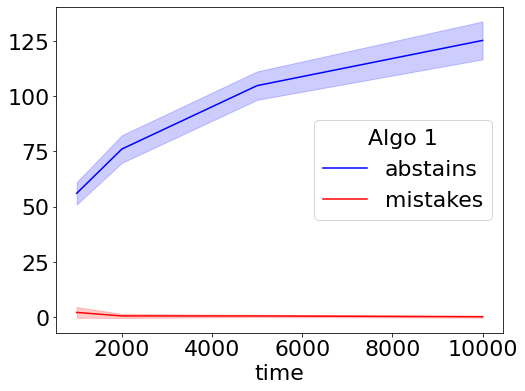
\includegraphics[width=\linewidth]{anomaly/figs/growth.png}
%   %\caption{Anomaly threshold set using a fixed cold-start period}
%   %\caption{}
%   %\label{fig:synthetic1}
% \end{subfigure}%
% \begin{subfigure}{.45\columnwidth}
%   \centering
%   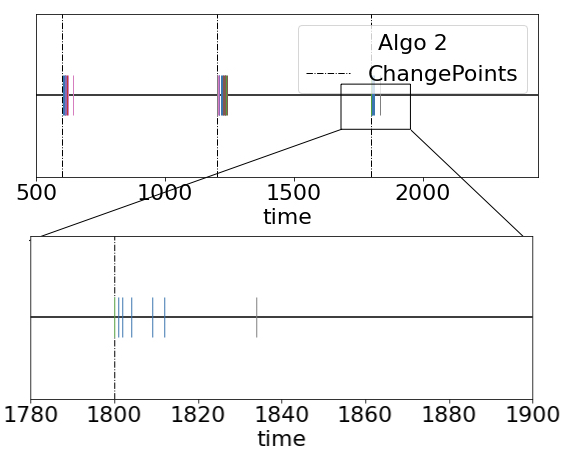
\includegraphics[width=\linewidth]{anomaly/figs/mistakes.jpeg}
%   %\caption{A subfigure}
%   %\caption{}
%   %\label{fig:synthetic2}
% \end{subfigure}
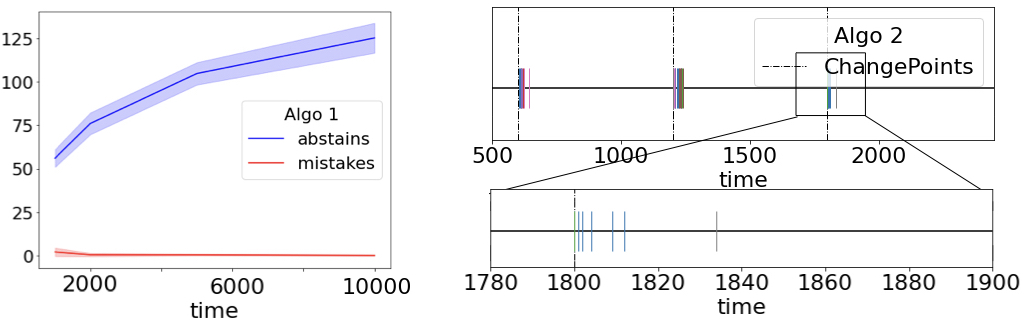
\includegraphics[width=0.95\linewidth]{anomaly/figs/exp1.jpeg}
\caption{\textit{Left:} algorithm 1, Abstains grows at $\gO(\sqrt{T})$. \textit{Right:}  algorithm 2, timestamp of mistakes in 10 random streams with aligned change points. Mistakes cluster right after change points, only as detection delay.}
\label{fig:synthetic}
\end{figure}

\subsection{MNIST anomaly detection}

We tested our algorithms on the MNIST dataset for one-class anomaly detection to demonstrate their real-world efficacy. We designated even digits as normal and odd digits as anomalous, and created data streams by sampling (e.g. Fig \ref{fig:mnist}). To show synergy of our thresholding algorithm with standard anomaly detection algorithms, we obtain anomaly scores from two models: convolutional autoencoder neural networks (NN) and isolation forests (IF), both trained on the normal class. With parameters set at $p = 0.99$ and $\alpha = 0.01$ for streams of 1000 samples, Table \ref{tab:mnist} illustrates our algorithm's improved performance over baselines.

\begin{table}[]
    \centering
    \begin{tabular}{l|c c||l | c c}
    \toprule
       Static  & abstains &  FP+FN  & Shift & abstains & FP+FN  \\
    \midrule
    $\tau^{30\%}$ & 327 \plusminus{0} & 12.7 \plusminus{0.9} &  $\tau^{30\%}$ & 670 \plusminus{0} & 91 \plusminus{8.0}\\
    DSpot & 150 \plusminus{0} & 78.1 \plusminus{2.5}  & DSpot & 150 \plusminus{0} & 129.5 \plusminus{10.2} \\
    IF+A1 & 172 \plusminus{16} & 17.6 \plusminus{5.3}  & IF+A3 & 190  \plusminus{39} & 75.7 \plusminus{18.9}\\
    NN+A1 & 133 \plusminus{4} & \textbf{3.9} \plusminus{0.7}  & NN+A3 & 339 \plusminus{12} & \textbf{9.3} \plusminus{2.1} \\
    NN+A5 & 89 \plusminus{6} & \textbf{2.1} \plusminus{0.2}  &  NN+A5 & 210 \plusminus{8} & \textbf{8.8} \plusminus{2.3} \\
    \bottomrule
    \end{tabular}
    \caption{One class MNIST result. We applied our algorithms (A as shorthand) to anomaly scores generated by Isolation Forest (IF) and neural networks (NN) and achieve much lower mistakes with moderate number of abstains. }
    \label{tab:mnist}
\end{table}

\begin{figure}
    \centering
    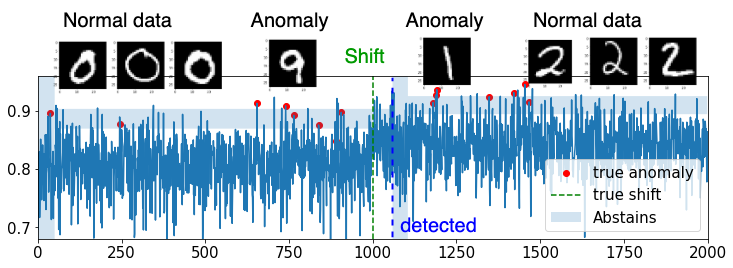
\includegraphics[width=0.9\linewidth]{anomaly/figs/Diagram2.png}
    \caption{MNIST experiment setup and a sample stream of (NN+A5) result. We choose a different set of digits for normal and anomaly to create the distribution shift, which our algorithm detects with a small delay. }
    \label{fig:mnist}
\end{figure}

\subsection{Case study of real AD application}

We also perform a case study on two real world datasets ({\ttfamily DS1} and {\ttfamily DS2}) obtained from large scale cloud computing services. Each dataset is a stream of anomaly scores obtained by applying the same black box anomaly detection algorithm (Details in Table \ref{tab:real_data_stats}). The practically motivated target in these datasets is to report $0.001\%$ anomalies, i.e., $p = 1-10^{-6}$.
Table \ref{tab:real_data} in the appendix reports the full result and comparison to baselines. We found that {\em(i)} our method achieves desired anomaly volume, {\em(ii)} incorporating offline data reduces the number of abstains without changing the volume of anomalies raised, and {\em(iii)} the volume of anomalies detected by all other methods are an order of magnitude higher leading to alert-fatigue. 


\section{Related Work}
\vspace{-0.2em}
\textbf{Dynamic thresholding for AD.} AD is an extensively researched topic, where a common paradigm is to first model data likelihood and then use a threshold to decide if a data point is normal or anomalous. This threshold is typically determined by an expert or offline through cross-validation \cite{luo2021deep, schmidl2022anomaly}. Dynamic and automatic methods makes AD algorithms more practical in real-world deployment \cite{ali2013automated, hundman2018detecting}, and are necessary where the data distribution can shift \cite{siffer2017anomaly}.  Our work is the first to provide abstain and mistake bounds on dynamic thresholding without assumptions on the underlying data distribution. Appendix \ref{app:related} contains more related work. %Using learned threshold to make binary decision of seeking labels from human experts are studied in active learning \cite{balcan2007margin, zhang2016online,vishwakarma2023promises}. However, active learning does not have a concept of mistakes and is thus different from ours. 

%\cite{siffer2017anomaly, , hundman2018detecting}
%This work instead focuses on providing a principled analysis of the thresholding step that follows. Traditionally, and are chosen by heuristics . Works closer to us are thresholding algorithms for univariate online streams .
%\vspace{-0.5em}
\textbf{Confidence Sequences (CS).} We incorporate theoretical results of confidence sequences \cite{ramdas2022game} in our analysis. \cite{maharaj2023anytime, howard2022sequential} derived the CS algorithm for estimating quantiles online with any-time guarantees, and \cite{shekhar2023sequential} leverages CS for detecting distribution shifts. 
\vspace{-0.5em}


\section{Discussion}

Our paper is the first to systematically theoretically and empirically show that thresholding algorithm can improve the overall performance of any anomaly scoring model for online anomaly detection. Through a simple argument (Theorem \ref{thm:main_lower_bound}), we demonstrate that abstaining is necessary for high accuracy. 

Our work introduces a new approach to online adaptive anomaly thresholding, leveraging CS to utilize offline data and dynamically adjust thresholds in real-time data streams. We give the first statistical guarantees on abstains and mistakes in various settings with non-stationary data streams and offline datasets (Theorem 2 - 6), motivated by practical AD applications. Our results are corroborated with synthetic and real experiments. %Future work can involve giving guarantees on threshold selection when the anomaly scores evolve through auto-regressive or temporal dependence. Another direction of future work is to relax Assumptions \ref{asumption_detectable} and \ref{defn:offline_datasets}.
%A limitation is that our results rely on assumptions of (1) samples are temporally independent and (2) change points are far apart and changes are detectable. Future work can involve giving guarantees on threshold selection when the anomaly scores evolve through auto-regressive or temporal dependence. 

A limitation of our work is that the theoretical results rely on (1) samples are temporally independent and (2) change points are far apart and changes are detectable. These assumptions, although standard in theoretical literature, need not necessarily hold in all applications.
Our algorithms also do not apply to cases when scores are temporal dependent, or if there are gradual drifts in the score distribution. Designing algorithms that provably work for these cases likely requires new techniques and is thus left for future work.

%Our insight is to use confidence sequences (CS) as both adaptive cold-start, as well as to test for distribution changes. Further, CS also enabled us to prove improved performance in the presence of offline datasets. 

%We address some possible questions and criticisms to our work. Our work abstracts away the modeling portion of anomaly detection, and instead focus on the decision making part. In this paper, we propose a new approach to thresholding; hence we consider challenges such as time-window, types of anomaly as beyond our scope. For estimating the quantiles, this work extensively uses \cite{howard2022sequential}'s confidence sequence method; their analysis focuses on estimation.  Our contribution lies in the algorithms and analyses of decision making regret given these estimations. Our algorithm is invariant to scale, offset, and occlusion. We are able to prove that algorithms fulfill the desiderata of AD outlined in section 1.2, and shown their effectiveness on large synthetic and real world datasets.

%Our setting, though uncommon in the anomaly detection literature, is motivated by practical use cases. In large cloud database/software systems, we often have a ``quota''  of anomaly alarms that we are allowed to send. How to decide which event to alarm while minimizing harmful events such as false positives and negatives becomes the research topic. As we have shown, our setting is neither simplistic or trivial \cite{wu2021current}, and our method achieve performance consistent with our theory on real datasets.



%%%%%%%%%%%%%%%%%%%%%%%%%%%%%%%%%%%%%%%%%%%%%%%%%%%%%%%%%%%%
%\clearpage



% \section{Corrections to the main paper}
% \begin{itemize}
%     \item Assumption \ref{asumption_detectable} has a mistake. We replaced the maximum $\max(D(\Delta_{k-1},\alpha), D(\Delta_{k},\alpha))$, by addition $D(\Delta_{k-1},\alpha) + D(\Delta_{k},\alpha)$.
%     \item Additional offline detectability assumption is needed in Section 5 and 6. We introduce them in the proofs as assumption \ref{as:offline_detectable} . See appendix F for details.
%     \item In Table 2, the column name ``Algo 4" should be ``Algo 3", the general algorithm. 
% \end{itemize}
% \vfill
\section{Illustrations}

We give schematic of the various settings and special cases studied in this paper. 

\begin{figure}[h!]
\centering
\begin{subfigure}{.45\columnwidth}
  \centering
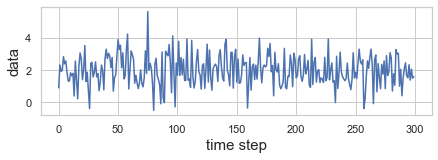
\includegraphics[width=\linewidth]{anomaly/figs/s1.png}
  \caption{Special Case I: stationary stream}
  \label{fig:s71}
\end{subfigure}%
\begin{subfigure}{.45\columnwidth}
  \centering
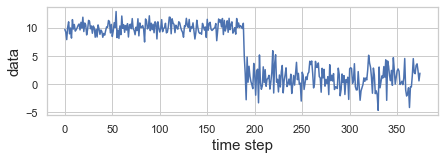
\includegraphics[width=\linewidth]{anomaly/figs/s2.png}
  \caption{Special Case II: distribution shift }
  \label{fig:s72}
\end{subfigure} \\
\begin{subfigure}{.45\columnwidth}
  \centering
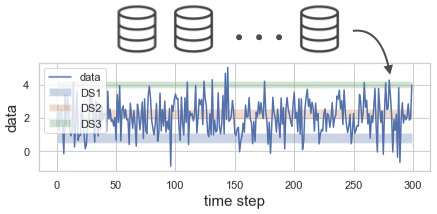
\includegraphics[width=\linewidth]{anomaly/figs/s3.jpeg}
  \caption{Special Case III: offline dataset }
\end{subfigure}%
\begin{subfigure}{.45\columnwidth}
  \centering
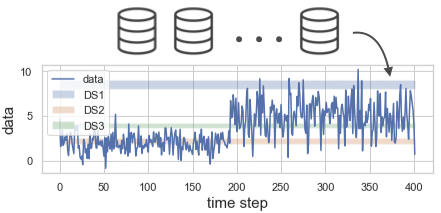
\includegraphics[width=\linewidth]{anomaly/figs/s4.jpeg}
  \caption{The General Case}
\end{subfigure}%
\caption{Illustration of the cases we study in this paper.}
\label{fig:setting_illustrations}
\end{figure}


\begin{figure}[h!]
    \centering
    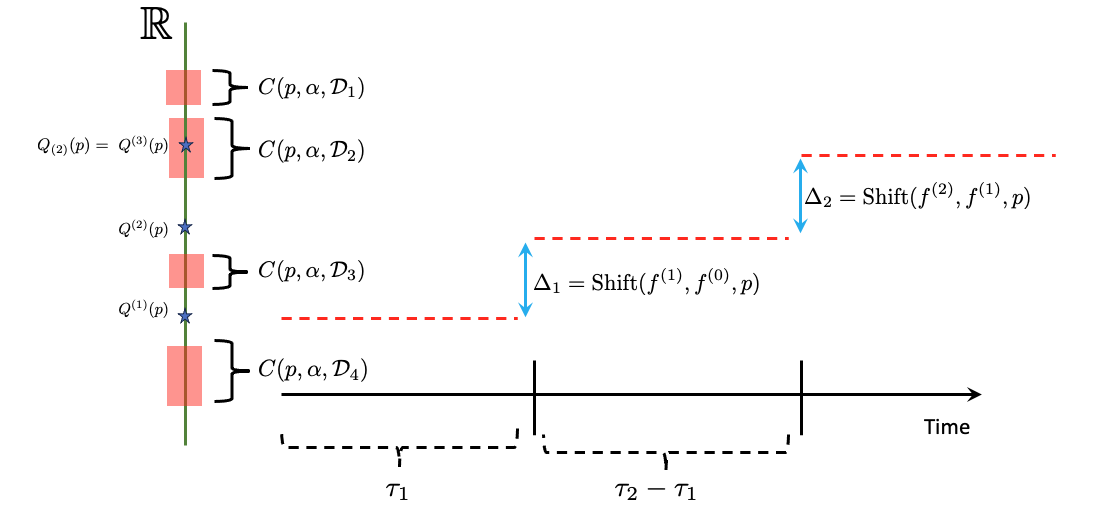
\includegraphics[width=0.8\linewidth]{anomaly/figs/separated_datasets.png}
    \caption{An illustration of Assumption \ref{asumption_detectable} and \ref{defn:offline_datasets} on a stream with $2$ change-points ($H_T=2)$ and $K=4$ offline datasets. Assumption \ref{asumption_detectable} implies that the change-points on the stream are sufficiently far apart. Assumption \ref{defn:offline_datasets} implies that the $4$ CS do not intersect. Moreover, either the true quantile on the stream are outside the offline CS, i.e., $Q^{(1)}(p)$ and $Q^{(2)}(p)$ are not contained in any offline dataset's CS. Or, it is the case that the online quantile matches one of the offline dataset, i.e., $Q_{(2)}(p) = Q^{(3)}(p)$ in this example.}
    \label{fig:separated_datasets_example}
\end{figure}

\pagebreak

\section{Proof of Theorem \ref{the:iid}, stationary setting}

\begin{algorithm}
\caption{OAD for stationary i.i.d. stream}\label{alg:one}
\SetKwInOut{Input}{Input}
\SetKwInOut{Output}{Output}
\Input{Quantile $p$, Confidence $1-\alpha$}
\Output{Anomaly labels $\hat{y}_1, \hat{y}_2, \ldots$}
\For{  $\text{each time }t \geq 1$ } {
    Receive $t^{th}$ input $S_t$\;
    
    Compute $C(p,\alpha, S_{1:t})$ (Eq. \ref{eq:cs})\;

    $\hat{y}_t \gets \text{{\ttfamily Algorithm }\ref{alg:marginal_decision}}(S_t, C(p,\alpha, S_{1:t}))$ \;
    
  %   %Compute $ub_t \gets \hat{Q}_t(p + u_t)$(Eq. \ref{eq:cs})\; 
  %   \uIf{$S_t > \max C(p,\alpha, S_{1:t})$}{
  %   $\hat{y}_t \gets1$\; \tcp{Declare an anomaly}
  % }
  % \uElseIf{$S_t \in C(p,\alpha , S_{1:t}$}{
  % $\hat{y}_t \gets * $ \; \tcp{Abstain from decision}
  % }
  % \Else{
  %   $\hat{y}_t \gets 0 $ \; \tcp{Declare benign}
  % }
}
\end{algorithm}

\begin{theorem}[Formal version of Theorem \ref{the:iid}]
If the data-source $S_1, S_2, \cdots$ are i.i.d., then with probability at-least $1-2\alpha$, for all times $T \in \mathbb{N}$, Algorithm \ref{alg:one} satisfies \begin{enumerate}
    \item $0$ False positives, $0$ False negatives
    \item Abstains is less than or equal to $7 \sqrt{T \ln \left( \frac{1612\ln(eT)}{\alpha^2} \right)}$,
    \item Abstains is at-least $\frac{1}{4} \sqrt{T \ln \left( \frac{1612\ln(eT)}{\alpha^2} \right)}$
    
\end{enumerate}
\label{the:iid_plus}
\end{theorem}
 
\begin{proof}
In order to give the proof, we set some notations. 

%
\begin{definition}[Good event $\gE_1$] %Denote the good event $\mathcal{E}_1$ as 
\begin{align}
\begin{split}
    \mathcal{E}_1 := \bigcap_{t \in \mathbb{N}} \bigcap_{p \in (0,1)} 
 \{  \widehat{Q}(p-u_t(\alpha), S_{1:t}) \leq Q(p) \leq \widehat{Q}(p+u_t(\alpha), S_{1:t}) \} .
\end{split}
\label{eqn:good_event_defn}
\end{align}   
\end{definition}
\vspace{-0.5em}
%
In words, the good event states that for all time $t$, the confidence sequence contains the true $p$th quantile.
From Corollary $2$ of \cite{howard2022sequential}, we know that $\mathbb{P}[\mathcal{E}] \geq 1-\alpha$. We remark that \cite{howard2022sequential} show that even when $(S_t)_{t \geq 1}$ are independent, but not necessarily identical, $\mathbb{P}[\mathcal{E}] \geq 1-\alpha$ holds as long as the $p$th quantile $Q_t(p) := Q(p)$ for all $t \geq 1$. This extension relaxing the identical distribution will be crucial in the subsequent sections in the sequel. 

Further, observe from the definition in Algorithm \ref{alg:one} and Equation (\ref{eq:cs}) that for all $t\in \mathbb{N}$ and $p \in (0,1)$,
\begin{align*}
     \{  \widehat{Q}(p-u_t(\alpha), S_{1:t}) \leq Q(p) \leq \widehat{Q}(p+u_t(\alpha), S_{1:t}) \} \subseteq \{ Q(p) \in C(p,\alpha, S_{1:t} \}.
\end{align*}

The reason for this inclusion is that the definition of $C(\cdot)$ in Equation (\ref{eq:cs}) has an extra factor of $2$, i.e., 
\begin{align*}
    C(p,\alpha,S_{1:t}) :=  \bigg[ \widehat{Q}(p- 2u_{n}(\alpha), y_{1:n}),  \widehat{Q}(p+2u_{n}(\alpha), y_{1:n}) \bigg].
\end{align*}


% Recall the good event $\mathcal{E}$ as defined in equation \ref{eqn:good_event_defn}.
% \begin{align*}
%     \mathcal{E} := \bigcap_{t \in \mathbb{N}} \bigcap_{p \in (0,1)} \{ Q(p) \leq \widehat{Q}_t(p+u_t) \} \bigcap \{ Q(p) \geq \widehat{Q}_t(p-u_t) \}.
% \end{align*}
% From Corollary $2$ of \cite{howard2022sequential}, we know that $\mathbb{P}[\mathcal{E}] \geq 1-\alpha$. 

In the rest of this proof, we will assume that the good event $\mathcal{E}$ holds. It is immediately clear the following two claims hold, proving the first two statements of the theorem.
\begin{claim}
If event $\mathcal{E}$ holds, then Algorithm 1 will not make any False Positive or False negative detections.
\label{claim:goodevent1}
\end{claim}

It now only remains to prove the third condition of the theorem. Define the sequence of indicator random variables indicating if time $t$ is an abstain
\begin{align} 
    Z_t := \mathbf{1}(\widehat{y}_t = *) .
\end{align} 

From Algorithm \ref{alg:one}, this is equivalent to 
\begin{align*}
    Z_{t} = \mathbf{1}(S_{t} \in (\widehat{Q}_t(p-2u_{t-1}(\alpha), S_{1:t-1}), \widehat{Q}_t(p+2u_{t-1}(\alpha), S_{1:t-1})).
\end{align*}
We denote by the filtration $(\mathcal{F}_t)_{t=1}^T$ to be generated by the observed sequence $(S_t)_{t=1}^T$, i.e., for all $t \in \{1,\cdots,T\}$, $\mathcal{F}_t := \sigma(S_1,\cdots,S_t)$. 


The proof of claim \ref{claim:goodevent1} follows from the following three lemmas. For clarity, proof for these lemmas can be found after this proof finishes.
 
% \begin{lemma}[Expectation of abstains] For every $t\geq2$, we have $\E(Z_t) \leq 3u_{t-1}(\alpha)$.
% \label{lem:exp_z}
% \end{lemma}

\begin{lemma}[Conditional expectation of abstains]
For every $ t \geq 2$, $$4u_{t-1}(\alpha) \leq \E[Z_t \mathbf{1}_{\mathcal{E}}| \mathcal{F}_{t-1}] \leq 6u_{t-1}(\alpha),$$ holds almost-surely.  
\label{lem:cond_exp}
\end{lemma}

\begin{lemma}[Azuma-Hoefding bound] 
Let $(Z_t)_{t=1}^T$ are bounded binomial variables and the sequence $(\mathcal{F}_t)_{t=1}^T$ is a probability filtration. Then for all $\varepsilon > 0$,
\begin{align*}
    \mathbb{P} \left[ \bigg| \sum_{s=1}^T Z_s  - \mathbb{E}[Z_s  \vert \mathcal{F}_{s-1}] \bigg| \geq \varepsilon \right] \leq 2 \exp \left( -\frac{ \varepsilon^2}{2T} \right)
\end{align*}
\label{lemma:azuma}
\end{lemma}

We now apply Lemma \ref{lemma:azuma} to the sequence of binary random variables $(\widetilde{Z}_t)_{t\geq 1} := (Z_t \mathbf{1}_{\mathcal{E}})_{t \geq 1}$ by setting $\varepsilon =  \sqrt{T \ln \left( \frac{4}{\alpha^2} \right)}$. Thus, with probability at least $1-\alpha$ %? $1-\frac{\alpha}{2}$
, we have

\begin{align*}
  \mathbb{P} \left[ \underbrace{ \bigg| \mathbf{1}_{\mathcal{E}} \sum_{s=1}^TZ_s - \sum_{s=1}^T \mathbb{E}[Z_s \mathbf{1}_{\mathcal{E}} \vert \mathcal{F}_{s-1}] \bigg| \leq   \sqrt{T \ln \left( \frac{4}{\alpha^2} \right)}}_{\text{Event } \mathcal{G}_1} \right] \geq 1- \alpha
  \end{align*}
  
From a simple union-bound argument, we see that $\mathbb{P}[\mathcal{E} \cap \mathcal{G}_1] \geq 1 - 2\alpha$. Furthermore by definition of event $\mathcal{G}_1$,  the following inequality holds almost-surely. 
\begin{align*}
    \mathbf{1}_{\mathcal{G}}\mathbf{1}_{\mathcal{E}_1} \sum_{s=1}^TZ_s &\leq \mathbf{1}_{\mathcal{G}_1}\left(\sum_{s=1}^T \mathbb{E}[Z_s \mathbf{1}_{\mathcal{E}} \vert \mathcal{F}_{s-1}] +  \sqrt{T \ln \left( \frac{4}{\alpha^2} \right)}\right),\\
        &\stackrel{\text{Lem } \ref{lem:cond_exp}}{\leq}  \mathbf{1}_{\mathcal{G}_1}\left( \sum_{t=1}^T 6u_{t-1}(\alpha) + \sqrt{T \ln \left( \frac{4}{\alpha^2} \right)}\right), \\
    &\stackrel{}{\leq}  \mathbf{1}_{\mathcal{G}_1}\left(6\sqrt{T \ln \left( \frac{1612 \ln(eT)}{\alpha} \right)} + \sqrt{T \ln \left( \frac{4}{\alpha^2} \right)}\right), \\
   &\leq  \mathbf{1}_{\mathcal{G}_1}\left(7\sqrt{T \ln \left( \frac{1612 \ln(eT)}{\alpha^2} \right)}\right).
\end{align*}
In other words, the preceding display reads that on the event $\mathcal{E} \cap \mathcal{G}_1$ holds, we have
  \begin{align*}
   \sum_{s=1}^TZ_s \leq 7\sqrt{T \ln \left( \frac{1612 \ln(eT)}{\alpha^2} \right)}.
\end{align*}
Similarly, from the definition of $\mathcal{G}_1$, we also have 
\begin{align*}
     \mathbf{1}_{\mathcal{G}}\mathbf{1}_{\mathcal{E}_1} \sum_{s=1}^TZ_s &\geq \mathbf{1}_{\mathcal{G}_1}\left(\sum_{s=1}^T \mathbb{E}[Z_s \mathbf{1}_{\mathcal{E}} \vert \mathcal{F}_{s-1}] -  \sqrt{T \ln \left( \frac{4}{\alpha^2} \right)}\right),\\
             &\stackrel{\text{Lem } \ref{lem:cond_exp}}{\geq}  \mathbf{1}_{\mathcal{G}_1}\left( \sum_{t=1}^T 2u_{t-1}(\alpha) - \sqrt{T \ln \left( \frac{4}{\alpha^2} \right)}\right), \\
    &\stackrel{}{\geq}  \mathbf{1}_{\mathcal{G}_1}\left(2\sqrt{T \ln \left( \frac{1612 \ln(eT)}{\alpha} \right)} - \sqrt{T \ln \left( \frac{4}{\alpha^2} \right)}\right), \\
   &\geq  \mathbf{1}_{\mathcal{G}_1}\left(\frac{1}{4}\sqrt{T \ln \left( \frac{1612 \ln(eT)}{\alpha^2} \right)}\right).
\end{align*}
The proof is complete since $\mathbb{P}[\mathcal{E} \cap \mathcal{G}_1] \geq 1-2\alpha$. 
\end{proof}


Below we provide the proof of each lemma used in proof of Theorem \ref{the:iid}. 

% \begin{proof}[Proof of Lemma \ref{lem:exp_z}]
% Note that again $\hat{Q}_t$ is the empirical quantile function of $\{S_i\}_{i=1}^{t-1}$. By exchangeability of i.i.d. samples, we know that the the probability of $S_t$'s rank among $\{S_i\}_{i=1}^{t-1}$ is uniform. Therefore,
% \begin{align*}
% \E(Z_t) = \prob (S_t \in [\hat{Q}(p-u_{t-1}(\alpha), S_{1:t-1}),\hat{Q}(p+u_{t-1}(\alpha),S_{1:t-1})])  \leq \frac{\ceil{2u_{t-1}(\alpha)\cdot (t-1)}}{t}  \leq  3u_t
% \end{align*}
% \end{proof}


\begin{proof}[Proof of Lemma \ref{lem:cond_exp}]
% In order to prove this result, we use the stornger Corollary $2$ of \cite{howard2022sequential}. We know from that corollary that if $g_t := 0.85\sqrt{t^{-1}(\log \log(et) + 0.8 \log (1612/\alpha))}$, then $$ \mathbb{P}[ \exists t \in \mathbb{N}, \exists p \in (0,1) : \{ Q(p) < \widehat{Q}_t(p-g_t) \} \cup  \{ Q(p) > \widehat{Q}_t(p + g_t) \} ] \leq  \alpha. $$
% Then in particular, we have
% {\color{black}
% \begin{align*}
%     \mathbb{P} \left[ \forall t, \{ Q(p+2u_t) \geq \widehat{Q}_t(p+u_t) \} \cap \text{  } \{ Q(p-2u_t) \leq \widehat{Q}_t(p-u_t) \} \right] \geq 1-\alpha. 
% \end{align*}
% }
% Thus, 
We can compute the conditional expectation as 
\begin{align*}
    \E[Z_t \mathbf{1}_{\mathcal{E}}| \mathcal{F}_{t-1}] 
    &= \mathbb{P}[S_t \in (\widehat{Q}(p-2u_{t-1}(\alpha),S_{1:t-1}), \widehat{Q}(p+2u_{t-1}(\alpha),S_{1:t-1}) ) \cap \mathcal{E} \vert \mathcal{F}_{t-1}], \\
        &\stackrel{(a)}{\leq}  \mathbb{P}[S_t \in (Q(p-3u_{t-1}(\alpha)), Q(p+3u_{t-1}(\alpha)) \vert \mathcal{F}_{t-1}]  \\
        &\stackrel{(b)}{\leq}  \mathbb{P}[S_t \in (Q(p-3u_{t-1}(\alpha)), Q(p+3u_{t-1}(\alpha)) ]  \\
    & \stackrel{(c)}{\leq} 6u_{t-1}(\alpha).
\end{align*}
Step $(a)$ follows from the fact that on event $\mathcal{E}$, for all times $t \in \mathbb{N}$ and quantiles $p \in (0,1)$, we have $Q(p) \leq \widehat{Q}(p+u_t(\alpha),S_{1:t})$ and $Q(p) \geq \widehat{Q}(p-u_t(\alpha),S_{1:t-1})$ holds. Step $(b)$ follows since $(S_t)_{t \geq 1}$ is an i.i.d. sequence and thus $S_t$ is independent of $\mathcal{F}_{t-1}$. Step $(c)$ follows from the standard fact the for any $\mathbb{R}$ valued continuous random variable, and for any quantiles $0 \leq p_1 \leq p_2 \leq 1 $, $\mathbb{P}[X \in (Q(p_1), Q(p_2))] = p_2 - p_1$.
Similarly, we have 
\begin{align*}
    \E[Z_t \mathbf{1}_{\mathcal{E}}| \mathcal{F}_{t-1}] 
    &= \mathbb{P}[S_t \in (\widehat{Q}(p-2u_{t-1}(\alpha),S_{1:t-1}), \widehat{Q}(p+2u_{t-1}(\alpha),S_{1:t-1}) ) \cap \mathcal{E} \vert \mathcal{F}_{t-1}], \\
        &\stackrel{(a)}{\geq}  \mathbb{P}[S_t \in (Q(p-u_{t-1}(\alpha)), Q(p+u_{t-1}(\alpha)) \vert \mathcal{F}_{t-1}]  \\
        &\stackrel{(b)}{\leq}  \mathbb{P}[S_t \in (Q(p-u_{t-1}(\alpha)), Q(p+u_{t-1}(\alpha)) ]  \\
    & \stackrel{(c)}{\leq} 2u_{t-1}(\alpha).
\end{align*}
follows from the fact that on event $\mathcal{E}$, for all times $t \in \mathbb{N}$ and quantiles $p \in (0,1)$, we have $Q(p) \leq \widehat{Q}(p+u_t(\alpha),S_{1:t})$ and $Q(p) \geq \widehat{Q}(p-u_t(\alpha),S_{1:t-1})$ holds. Step $(b)$ follows since $(S_t)_{t \geq 1}$ is an i.i.d. sequence and thus $S_t$ is independent of $\mathcal{F}_{t-1}$. Step $(c)$ follows from the standard fact the for any $\mathbb{R}$ valued continuous random variable, and for any quantiles $0 \leq p_1 \leq p_2 \leq 1 $, $\mathbb{P}[X \in (Q(p_1), Q(p_2))] = p_2 - p_1$.
\end{proof}

\begin{proof}[Proof of Lemma \ref{lemma:azuma}]
Denote by the sequence of $0$ mean random variables $\widetilde{Z}_t := Z_t - \mathbb{E}[Z_t \vert \mathcal{F}_{t-1}]$. Denote by the running sum $Y_t := \sum_{s=1}^{t} \widetilde{Z}_s$. It is easy to verify that $(Y_t)_{t=1}^T$ is a martingale sequence. Further from definition, we have have that almost-surely, for all $t \in \{1,\cdots, T\}$, $|Y_{t} - Y_{t+1}| \leq 2$. Thus, from Azuma Hoeffding inequality for bounded martingales, we have that 
\begin{align}
    \mathbb{P}\left[\sum_{s=1}^T \widetilde{Z}_s \geq \sqrt{T \ln \left( \frac{4}{\alpha^2} \right)}\right] &\leq 2 \exp \left( - \frac{2 T \ln \left( \frac{4}{\alpha^2} \right)}{4T} \right), \\
    &\leq \frac{\alpha}{2}.
\end{align}


\end{proof}

\section{Proofs from Section \ref{sec:offline-only}}



The proofs in this section are dependent on the following good-event, under which we will perform the analysis.

%\subsection{Good events for quantile estimation}

\begin{definition}[Good event 2] 
Let $(S_t)_{t=1}^T \sim \Bigl(T,H_T, (\tau_c)_{c=0}^{H_T}, (f^{(c)})_{c=0}^{H_T}\Bigr)$, with quantile functions of the $H_T+1$ segments given by $(Q^{(c)}(\cdot))_{c=0}^{H_T}$. Define $\gE_2$ as
\begin{align}
    \widehat{\gE_2} := \bigcap_{k=1}^{H_T} \gE_2^{(k)},
    \label{eqn:good_event_2_defn_internal}
\end{align}
where for each $k \in [H_T]$, 
\begin{align*}
        \mathcal{E}_2^{(k)} =  \bigcap_{p \in [0,1]} \bigcap_{t_1 = \tau_{k}}^{\tau_{k+1}} \bigcap_{t_2 = t_1 +1}^{\tau_{k+1}}   \bigg\{ \widehat{Q}(p-u_{t_2 - t_1}(\alpha), S_{t_1:t_2})  \leq Q^{(k)}(p) \leq \widehat{Q}(p-u_{t_2 - t_1}(\alpha), S_{t_1:t_2}) \bigg\},
\end{align*}
where $\widehat{Q}$ is the empirical quantile and $u_{(\cdot)}(\cdot)$ is defined in Equation (\ref{eqn:defn_confidence_width_ut}).
\label{as:goodevent2}
\end{definition}
%\vspace{-1em}
%
In words,  $\gE_2$ is the intersection over all the $H_T+1$ stationary segments, where for each segment the quantile estimate is close to the true quantile for all quantiles. Following Corollary $2$ of \cite{howard2022sequential} and an union bound, we get the following.

\begin{proposition}
    \begin{align*}
        \mathbb{P}[\widehat{\gE_2}] \geq 1 - T\alpha.
    \end{align*}
    \label{prop:good_event_2_prob_hat}
\end{proposition}
\begin{proof}
    We analyze the complement as follows.
    \begin{align*}
        & \quad \; \mathbb{P}[\widehat{\gE_2}^{\complement}] \\ &= \mathbb{P} \left[ \cup_{k=0}^{H_T} \cup_{p \in [0,1]} \cup_{t_1=\tau_k}^{\tau_{k+1}} \cup_{t_2 \geq t_1 + 1} \{ \widehat{Q}(p-u_{t_2 - t_1}(\alpha), S_{t_1:t_2})  > Q^{(k)}(p) \} \cup \{ Q^{(k)}(p) > \widehat{Q}(p-u_{t_2 - t_1}(\alpha), S_{t_1:t_2}) \}  \right], \\
        &\leq \sum_{k=0}^{H_T} \sum_{t_1=\tau_k}^{\tau_{k+1}}\mathbb{P} \left[ \cup_{p \in [0,1]} \cup_{t_2 \geq t_1 + 1} \{ \widehat{Q}(p-u_{t_2 - t_1}(\alpha), S_{t_1:t_2})  > Q^{(k)}(p) \} \cup \{ Q^{(k)}(p) > \widehat{Q}(p-u_{t_2 - t_1}(\alpha), S_{t_1:t_2}) \}  \right], \\
        &\stackrel{(a)}{\leq}\sum_{k=0}^{H_T} \sum_{t_1=\tau_k}^{\tau_{k+1}}\alpha, \\
        &= T \alpha.
    \end{align*}
    Step $(a)$ follows from   Corollary $2$ of \cite{howard2022sequential}.
\end{proof}

{\color{black}

In addition, we also need a generalization of event $\mathcal{G}_1$ to the piece-wise stationary stream. 

\begin{align}
  \gG_2:=  \bigcap_{k=0}^{H_T} \bigcap_{t_1 = \tau_k + 1}^{\tau_{k+1}}\bigg\{ \bigg| \sum_{t=t_1}^{\tau_{k+1}}Z_{t:t_1} - \mathbb{E}[Z_{t:t_1} \vert \mathcal{F}_{t-1}] \bigg| \leq \sqrt{(\tau_{k+1} - \tau_k) \ln \left( \frac{4}{\alpha^2} \right)} \bigg\},
  \label{eqn:good_event_G}
\end{align}
where 
\begin{align}
    Z_{t:t_1} := \mathbf{1}(S_{t} \in (\widehat{Q}_t(p-2u_{t-t_1}(\alpha), S_{t_1:t-1}), \widehat{Q}_t(p+2u_{t-t_1}(\alpha), S_{t_1:t-1})),
\end{align}
and $\mathcal{F}_{t-1} := \sigma(S_{1:t-1})$ is the sigma-algebra generated by the first $t-1$ samples.

\begin{proposition}
    \begin{align*}
        \mathbb{P}[\gG_2] \geq 1 - T \alpha.
    \end{align*}
    \label{prop:abstain_good_event}
\end{proposition}
For a given $k$ and $t_1$, the proof follows from an application of Azuma-Hoeffding similar to the proof of Theorem \ref{the:iid}. Applying an union bound over $k$ and $t_1$ yields the result. 

In the rest of this section, denote the good event $\gE_2$ as 
\begin{align}
    \gE_2 = \widehat{\gE_2} \bigcap \gG_2,
    \label{eqn:good_event_2_defn}
\end{align}
where $\widehat{\gE}_2$ is defined in Equation (\ref{eqn:good_event_2_defn_internal}) and $\gG_2$ in Equation (\ref{eqn:good_event_G}).

\begin{proposition}
    \begin{align*}
        \mathbb{P}[\widehat{\gE_2}] \geq 1 - T\alpha.
    \end{align*}
    \label{prop:good_event_2_prob}
\end{proposition}
The proof follows from an union bound using estimates in Proposition \ref{prop:good_event_2_prob_hat} and \ref{prop:abstain_good_event}.

}

\subsection{Proof of Proposition \ref{prop:delay_bound}}


\begin{figure}[h!]
    \centering
    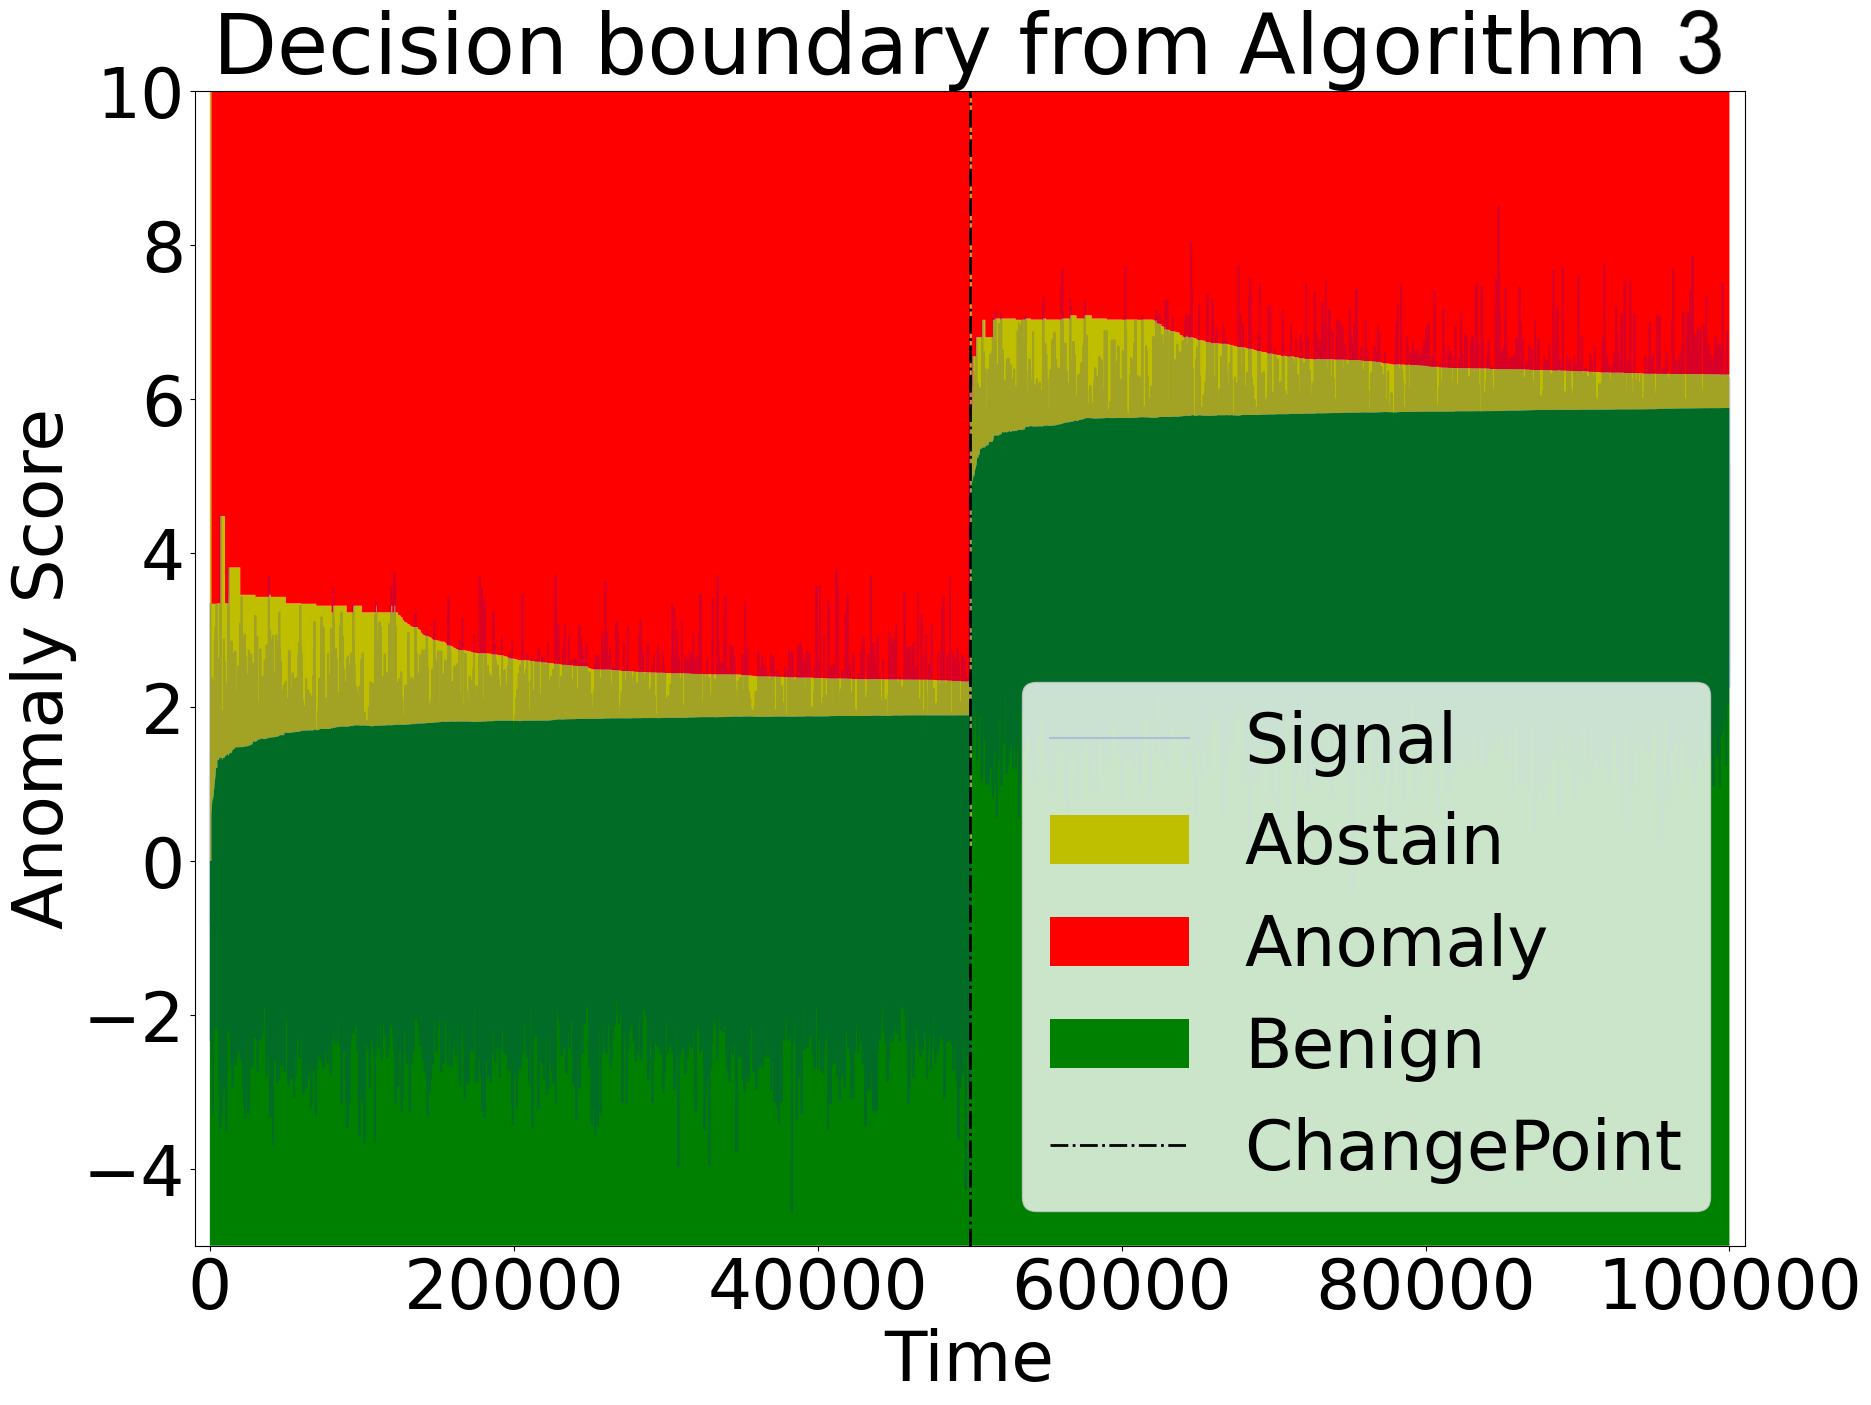
\includegraphics[width=0.4\linewidth]{anomaly/figs/algo_2_example.png}
    \caption{Algorithm 3 output on a piece-wise stationary stream.}
    \label{fig:s1}
\end{figure}

In order to give the proof of Proposition \ref{prop:delay_bound}, we need the following general lemma on change-detection. 


\begin{proposition}[Stream with a single change-point]
Let $(S_t)_{t=1}^T$ be a piecewise stationary stream with a single change-point, i.e., $H_T = 1$ with the change-point instant $\tau_1 = \tau \in [T]$. Denote by $\Delta := \text{Shift}(f^{(0)}, f^{(1)}, p)$ as the distribution shift magnitude. Denote by $\tau' \in \mathbb{N}$ as the first time when the {\ttfamily if} statement in Algorithm \ref{alg:two} evaluates to {\ttfamily True}, i.e., a change is detected for the first time by Algorithm \ref{alg:two}. Then, under the good event  $\gE_2$  (Definition \ref{as:goodevent2}), 
\begin{align*}
    \tau \leq \tau' 
    &\leq \bigg\lceil \inf_{\widetilde{\tau}} \left\{  u_{\tau}(\alpha) + u_{\widetilde{\tau}-\tau}(\alpha) \leq \frac{\Delta}{6} \right\} \bigg\rceil,
\end{align*}
where $u_t(\alpha)$ is given in Equation (\ref{eqn:defn_confidence_width_ut}). 
\label{prop:dist_changes}
\end{proposition}


We recall some notation to give the proof. The two distributions are denoted by $f^{(0)}$ and $f^{(1)}$ and their corresponding quantile functions are given by $Q^{(0)}(\cdot)$ and $Q^{(1)}(\cdot)$, where for $i \in \{0,1\}$, the function $Q^{(i)}(\cdot) : [0,1] \to \mathbb{R}$ is such that for all $p \in [0,1]$, $Q^{(i)}(p)$ is the $p$th quantile of the distribution $f^{(i)}$. Since we assume all distributions are continuous, the existence and uniqueness of quantile functions are granted. 

\textbf{Proof that $\tau \leq \tau'$}

Observe that under the event $\gE_2$, we have for all $t_1 < t_2 \in [\tau]$, $Q^{(0)}(p) \in C(p,\alpha, S_{t_1:t_2})$. Thus, for all $t \in [\tau]$, $Q^{(0)}(p) \in \bigcap_{s=1}^t C(p,\alpha,S_{s:t}) \bigcap_{s=1}^t C(p,\alpha,S_{1:s})$, and in particular, $\bigcap_{s=1}^t C(p,\alpha,S_{s:t}) \bigcap_{s=1}^t C(p,\alpha,S_{1:s})$ is non-empty. Therefore, under event $\gE_2$, for all $t \in [\tau]$, Algorithm \ref{alg:change_point} will never return {\ttfamily True} for the input sequence $S_{1:t}$.

\textbf{Proof on the upper bound of $\tau'$}

Since $\Delta > 0$, we will assume here that $Q^{(0)}(p) < Q^{(1)}(p)$ and this is without loss of generality since the proof for the other case follows identically. 
To prove the upper bound, it suffices to prove that if event $\gE_2$ holds and no change is detected till time $\tau' = \inf \{\widetilde{\tau}: u_{\tau}(\alpha)+ u_{\widetilde{\tau}-\tau}(\alpha) \}$, then at time $\lceil \tau' \rceil$, a change point will be detected. 

In order to prove this, we need to establish that $\bigcap_{s=1}^{\lceil \tau' \rceil} C(p,\alpha,S_{s:t}) \bigcap_{s=1}^{\lceil \tau' \rceil} C(p,\alpha,S_{1:s}) = \emptyset$. A sufficient condition for this is to prove that $C(p,\alpha,S_{\tau+1:\lceil \tau' \rceil}) \bigcap C(p,\alpha,S_{1:\tau}) = \emptyset$, i.e., the following implication holds 
\begin{align}
    C(p,\alpha,S_{\tau+1:\lceil \tau' \rceil}) \bigcap C(p,\alpha,S_{1:\tau}) = \emptyset \implies \bigcap_{s=1}^{\lceil \tau' \rceil} C(p,\alpha,S_{s:t}) \bigcap_{s=1}^{\lceil \tau' \rceil} C(p,\alpha,S_{1:s}) = \emptyset.
    \label{eqn:setting_2_internal_implication}
\end{align}
From Equation (\ref{eq:cs}), we know that 
\begin{align*}
     C(p,\alpha,S_{1:\tau}) = \bigg[ \widehat{Q}(p-2u_{\tau}(\alpha), S_{1:\tau}), \widehat{Q}(p+2u_{\tau}(\alpha), S_{1:\tau}) \bigg].
\end{align*}

Since event $\gE_2$ holds, it follows that 
\begin{align}
    \widehat{Q}(p+2u_{\tau}(\alpha),S_{1:\tau}) &\leq Q^{(0)}(p+3u_{\tau}(\alpha))     \label{eqn:setting_2_delay_pf_11}\\
    \widehat{Q}(p-2u_{\lceil \tau' \rceil - \tau}(\alpha)) &\geq Q^{(1)}(p - 3u_{\lceil \tau' \rceil-\tau}(\alpha)).
    \label{eqn:setting_2_delay_pf_1}
\end{align}
Further, from the definition of $\Delta$ in Definition \ref{def:quantile_shift} and the assumption that $Q^{(0)}(p) < Q^{(1)}(p)$ we know that 
\begin{align}    
Q^{(0)}( p + {\Delta} ) \leq Q^{(1)}(p - {\Delta})
    \label{eqn:setting_2_delay_pf_2}
\end{align}

Now, from the definition of $\tau'$, we know that 
\begin{align}
    3(u_{\tau}(\alpha) + u_{\lceil {\tau'} \rceil-\tau}(\alpha)) \leq {\Delta}
        \label{eqn:setting_2_delay_pf_3}
\end{align}

Now, combining the inequalities in Equations (\ref{eqn:setting_2_delay_pf_1}, \ref{eqn:setting_2_delay_pf_2}, \ref{eqn:setting_2_delay_pf_3}), we get that 
\begin{multline}
\widehat{Q}(p+2u_{\tau}(\alpha),S_{1:\tau}) \stackrel{\ref{eqn:setting_2_delay_pf_11}}{\leq} Q^{(0)}(p+3u_{\tau}(\alpha)) \stackrel{(a)}{<} Q^{(0)}(p+3u_{\tau}(\alpha) + 3u_{\lceil {\tau'} \rceil-\tau}(\alpha)) \stackrel{\ref{eqn:setting_2_delay_pf_3}}{\leq} Q^{(0)}(p+{\Delta}) \stackrel{\ref{eqn:setting_2_delay_pf_2}}{\leq} \\ Q^{(1)} ( p - {\Delta} ) \stackrel{\ref{eqn:setting_2_delay_pf_3}}{\leq} Q^{(1)}(p-3u_{\lceil {\tau'} \rceil-\tau}(\alpha)) \stackrel{\ref{eqn:setting_2_delay_pf_1}}{\leq} \widehat{Q}(p-2u_{\tau}(\alpha),S_{\tau:\lceil {\tau'} \rceil}).
\label{eqn:disjoint}
\end{multline}
Step $(a)$ follows from the fact that since $f^{(0)}$ and $f^{(1)}$ are a continuous distribution, we have for all $i \in \{0,1\}$ and a;; $0 < p_1 < p_2 < 1$, $Q^{(i)}(p_1) < Q^{(i)}(p_2)$. Thus, Equation (\ref{eqn:disjoint}) gives that under the event $\gE_2$, $   C(p,\alpha,S_{\tau+1:\lceil \tau' \rceil}) \bigcap C(p,\alpha,S_{1:\tau}) = \emptyset$, which from Equation (\ref{eqn:setting_2_internal_implication}) implies that if Algorithm \ref{alg:change_point} is queried with input $S_{1:\lceil \tau' \rceil}$, will return a {\ttfamily 1}, i.e., detect a change-point.


\textbf{Concluding the proof of Proposition \ref{prop:delay_bound} as an application of Proposition \ref{prop:dist_changes}}

% \begin{proposition*}[\ref{prop:delay_bound}]
% If the number of pre-change samples $\tau \geq \frac{20}{\Delta^2}\ln \left( \frac{1612}{\alpha \Delta^2}\right)$, then $\text{Delay}(\tau, \Delta, \alpha) \leq \frac{20}{\Delta^2}\ln \left( \frac{1612}{\alpha \Delta^2}\right).$
% \end{proposition*}

\begin{proof}
% Let $\tau$ denote the number of pre-change samples, and let $\tau'$ denote the point where the changes are detected. Delay can be defined as $\tau' - \tau$.  Suppose $\tau \geq \frac{20}{\Delta^2}\ln \left( \frac{1612}{\alpha \Delta^2}\right)$.

% For a change of magnitude $\Delta$ with $\tau$ pre-change samples to be detectable under the good event $\gE_2$, a \emph{sufficient} condition is that the forward and backward confidence sequences becomes disjoint at time $\tau$:
% \begin{align}
%     2(u_{\tau}(\alpha) + u_{\tau'- \tau}(\alpha)) \leq \Delta
% \label{eq:detectability}
% \end{align}

The proof rests on the following numerical claim.

\begin{claim}
If $\tau \geq \frac{80}{\Delta^2}\ln \left( \frac{1612}{\alpha \Delta^2}\right)$, then $u_\tau(\alpha) \leq \Delta/6 $ holds.
\label{claim:delay1}
\end{claim}
{\color{black}
\begin{proof}[Proof of Claim \ref{claim:delay1}]
Suppose $\tau \geq \frac{80}{\Delta^2}\ln \left( \frac{1612}{\alpha \Delta^2}\right)$. Then
\begin{align*} 
    u_{\tau}(\alpha) &\leq \sqrt{\frac{\ln \left( \frac{1612}{\alpha}(1+\ln(\tau)) \right)}{\tau}}, \\
    &\leq \frac{\Delta}{6}  \frac{\sqrt{{\ln \left( \frac{1612}{\alpha}(1+\ln(\tau)) \right)}}}{\sqrt{5\ln \left( \frac{1612}{\alpha \Delta^2} \right)}}, \\
    &\leq \frac{\Delta}{6} \frac{\sqrt{\ln \left( \frac{1612}{\alpha}\left(1+\ln\left(\frac{20}{\Delta^2}\ln \left( \frac{1612}{\alpha \Delta^2} \right)\right)\right) \right)}}{{\sqrt{5\ln \left( \frac{1612}{\alpha \Delta^2} \right)}}}, \\
    &\leq \frac{\Delta}{6}.
\end{align*}
\end{proof}

Applying Claim 2 to both $\tau$ and $\tau' - \tau$ allows use to satisfy the condition in Proposition \ref{prop:delay_bound}.

\begin{align*}
    & \tau \geq  \frac{80}{\Delta^2}\ln \left( \frac{1612}{\alpha \Delta^2}\right), \; \lceil \tau' \rceil - \tau \geq  \frac{80}{\Delta^2}\ln \left( \frac{1612}{\alpha \Delta^2}\right) \\
\Longrightarrow \;\; & u_{{\tau}}(\alpha) \leq \Delta/6, \; u_{{\lceil \tau' \rceil-\tau}}(\alpha) \leq \Delta/6, \\
\Longrightarrow \;\; & 3(u_{{\tau}}(\alpha)+ u_{{\lceil \tau' \rceil-\tau}}(\alpha)) \leq \Delta
\end{align*}

%Note that  $\tau' = \tau + \text{Delay}(\tau, \Delta, \alpha)$; we obtain $\text{Delay}(\tau, \Delta, \alpha) \leq \frac{80}{\Delta^2}\ln \left( \frac{1612}{\alpha \Delta^2}\right)$ by substituting the result above.  
}
\end{proof}



\subsection{Proof of Theorem \ref{thm:online_shift}}

% \begin{theorem*}[ \ref{thm:online_shift}]
% Let $(S_t)_{t = 1}^T$ be generated from a piece-wise stationary process $\Bigl(T,H_T, (\tau_c)_{c=0}^{H_T}, (f_c)_{c=0}^{H_T}\Bigr)$ with quantile shifts  $\Delta_{k} := \text{Shift} (f_{k},f_{k+1})$, $\forall k \in [1,H_T]$. With probability at-least $1-T\alpha$, Algorithm \ref{alg:two} satisfies 
% \begin{itemize}
%     \item False positive and false negative satisfy 
%     \[\text{FP} + \text{FN}  \leq \sum_{k=1}^{H_T}D(\Delta_{k},\alpha) = H_t \cdot {\gO}(\frac{1}{(\Delta_{min})^2}) 
%     \]
%     \item Number of abstains less than 
%     \begin{align*}
%         \sum_{k=1}^{H_T} \Bigl[ &4 \sqrt{(\tau_k-\tau_{k-1}) \ln \left( \frac{1612}{\alpha^2} \ln(e(\tau_k-\tau_{k-1})) \right)} + D(\Delta_{k},\alpha) \Bigr]
%     \end{align*}
% \end{itemize}
% where $D(\Delta_{k},\alpha)$ is defined in Equation (\ref{eq:delay_shorthand}).
% \end{theorem*}

\begin{theorem*}[ \ref{thm:online_shift}]%[Bounds for setting 2, algorithm \ref{alg:two}]
Let $(S_t)_{t = 1}^T \sim \Bigl(T,H_T, (\tau_c)_{c=0}^{H_T}, (f_c)_{c=0}^{H_T}\Bigr)$ be  a piece-wise stationary data-stream satisfying Assumption \ref{asumption_detectable} for $\alpha \in (0,1)$. Then, with probability at-least $1-2T\alpha$, Algorithm \ref{alg:two} satisfies {\em both}
\begin{itemize}
    \item $\text{FP} + \text{FN}  \leq \sum_{k=1}^{H_T}D(\Delta_{k},\alpha) = H_T \cdot {\gO}(\frac{1}{(\min_k\Delta_{k})^2}) $, 
    \item Number of abstains $ \leq \sum_{k=1}^{H_T} \Bigl[ 7 \sqrt{(\tau_k-\tau_{k-1}) \ln \left( \frac{1612}{\alpha^2} \ln(3(\tau_k-\tau_{k-1})) \right)}  + D(\Delta_{k},\alpha) \Bigr]$,
\end{itemize}
where for all $k \in [H_T]$, $\Delta_{k} = \text{Shift} (f^{(k)},f^{(k-1)},p)$  is the quantile shift defined in Definition (\ref{def:quantile_shift}) and $D(\cdot,\cdot)$ is defined in Equation (\ref{eq:delay_shorthand}).
%\label{thm:online_shift}
\end{theorem*}




At a high-level, the proof idea is to show in Lemma \ref{lem:bdd_delay_change_induction} that if Assumption \ref{asumption_detectable} holds, then under the good event in Equation (\ref{eqn:good_event_2_defn}) {\em (i)} there are no false positive detections, and {\em (ii)} all the true changes are detected with bounded delay. This will conclude the proof of Theorem \ref{thm:online_shift} since a simple union bound over Corollary $2$ of \cite{howard2022sequential} implies that the good event in Equation (\ref{eqn:good_event_2_defn}) holds with probability at-least $1-T \alpha$.

In order to formalize the proof, we recall notations. As before, denote by $\tau_1 < \tau_2 \cdots < \tau_k < \tau_{k+1}$ be the set of times at which a true-change occurs. For each $k \in \{1, \cdots, H_T\}$, denote by $\tau'_k$ as the time at which Algorithm \ref{alg:two} detects a change for the $k$th time. The first observation is the lemma below which states that there are no false positives and the delay of all change detections are bounded.


% \begin{lemma}[No False Positives]
%      Under the event $\mathcal{E}_2$, $\tau_k^{'} \geq \tau_k$ holds for all $k \in \{1, \cdots, H_T\}$.
%      \label{lem:no_fp_in_change}
% \end{lemma}

\begin{lemma}[No false detections and bounded delay]
    Under the event $\mathcal{E}_2$, if Assumption \ref{asumption_detectable} holds, then for all $k \in \{1, \cdots, H_T\}$, 
    \begin{itemize}
        \item  $\tau'_k \geq \tau_k$, and
        \item $\tau'_k - \tau_k \leq D(\Delta_k, \alpha)$.
    \end{itemize}
    \label{lem:bdd_delay_change_induction}
\end{lemma}

Before giving the proof of the lemma, we show how it concludes the Proof of Theorem \ref{thm:online_shift}.

\begin{proof}[Proof of Theorem \ref{thm:online_shift}]
    
We can break down the analysis by change points, because we know that all changes are detected before the next change occurs. Moreover, Algorithm \ref{alg:two} restarts a fresh copy of Algorithm \ref{alg:one} after each change point is detected, and thus we can use the guarantees given in Theorem \ref{the:iid}.

Consider a subset of time points $[S_{\tau_k}, S_{\tau_{k+1}}]$ for some $ k\in[1,H_T]$. We will denote the time step of detecting change point $\tau_k$,  as $\tau'_k$.  The total number of mistakes (false positives and false negatives) is the sum of mistakes before and after $\tau'_k$. Therefore under the good event $\gE_2$ we have:

\begin{align*}
    \text{FP} + \text{FN} &= \sum_{k=0}^{H_T} \left( \sum_{t=\tau_k}^{\tau'_k} \mathbf{1}(\text{Time $t$ is a mistake)} + \sum_{t=\tau'_k + 1}^{\tau_{k+1}} \mathbf{1}(\text{Time $t$ is a mistake)} \right) \\
    %&\sum_{k=0}^{H_T}  [\text{mistakes}(S_{\tau_k:\tau'_k}) + \text{mistakes}(S_{\tau'_k:\tau_{k+1}})] \\ 
    &\leq \sum_{k=0}^{H_T} (\tau'_k - \tau_k) + 0 \quad \quad \text{(Event $\gE_2$ definition in Equation (\ref{eqn:good_event_2_defn}))}\\
    &\leq \sum_{k=0}^{H_T} D(\Delta_k, \alpha) + 0 \quad \quad \text{(Lemma \ref{lem:bdd_delay_change_induction})}\\
\end{align*}

%The last inequality follows since Lemma \ref{lem:bdd_delay_change_induction} gives that $\tau_k^{'} - \tau_k \leq D(\Delta_k, \alpha)$ and Theorem \ref{the:iid} gives that Algorithm \ref{alg:one} incurs no FP or FN under event $\mathcal{E}_1$. 
The analysis is similar for number of abstains. 
\begin{align*}
    \text{Abstains}  &= \sum_{k=0}^{H_T} \left( \sum_{t=\tau_k}^{\tau'_k} \mathbf{1}(\text{Time $t$ is abstained)} + \sum_{t=\tau'_k + 1}^{\tau_{k+1}} \mathbf{1}(\text{Time $t$ is abstained)} \right) \\
    %&= \sum_{k=0}^{H_T} [\text{abstains} (S_{\tau_k:\tau'_k}) + \text{abstains}(S_{\tau'_k:\tau_{k+1}})] \\
    &\leq \sum_{k=0}^{H_T} \left[(\tau_{k}' - \tau_k) + \sum_{t=\tau'_k + 1}^{\tau_{k+1}} \mathbf{1}(\text{Time $t$ is abstained)}\right] \\
    &\stackrel{\text{Lemma \ref{lem:bdd_delay_change_induction}}}{\leq} \sum_{k=0}^{H_T} 
    \Bigl[ D(\Delta_k, \alpha) + \sum_{t=\tau'_k + 1}^{\tau_{k+1}} \mathbf{1}(\text{Time $t$ is abstained)} \Bigr], \\
     &\stackrel{(a)}{\leq} \sum_{k=0}^{H_T} 
    \Bigl[ D(\Delta_k, \alpha) + \sum_{t=\tau_k' + 1}^{\tau_{k+1}} \mathbf{1}(Z_{t:\tau'_k}=1) \Bigr], \\
         &\stackrel{(b)}{\leq} \sum_{k=0}^{H_T} 
    \Bigl[ D(\Delta_k, \alpha) +  7 \sqrt{(\tau_k-\tau_{k-1}) \ln \left( \frac{1612}{\alpha^2} \ln(3(\tau_k-\tau_{k-1})) \right)}  \Bigr].
\end{align*}
In step $(a)$, we use the definition of $Z_{t:t_1}$ as used in Equation (\ref{eqn:good_event_G}) and in step $(b)$, we use the fact that event $\gG_2$ holds and thus the calculations from Theorem \ref{the:iid} can be used. 
\end{proof}

\subsection{Proofs of Lemma  \ref{lem:bdd_delay_change_induction}}

%\begin{proof}[Proof of Lemma \ref{lem:no_fp_in_change}]
We prove the result by induction on $k \in \{1,\cdots, H_T\}$. 

\textbf{Base case of $k=1$}: 
Observe that under event $\mathcal{E}_2$, we have $\tau_1^{'} \geq \tau_1$. This is so since for all times $t \in \{1,\cdots, \tau_1\}$, there will be no distribution-shift detected, since by definition under event $\mathcal{E}_2$, the forward and backward CS will contain at-least the true quantile and will thus be non-empty. 

Now, under Assumption \ref{asumption_detectable}, we know that $\tau_1 \geq \frac{20}{\Delta_1^2}\ln \left( \frac{1612}{\alpha \Delta_1^2}\right)$. Thus, by Proposition \ref{prop:delay_bound}, we know that $\tau_1^{'} - \tau_1 \leq \frac{20}{\Delta_1^2}\ln \left( \frac{1612}{\alpha \Delta_1^2}\right) := D(\Delta_1, \alpha)$, where the last equality is from  definition in Equation (\ref{eq:delay_shorthand}). This proves the induction base case. 

\textbf{Induction hypothesis}: Now, assume that for some $k \in \{1,\cdots, H_t\}$, we have that $\tau_{k}^{'} - \tau_k \leq D(\Delta_k, \alpha)$. We will now show that the $(k+1)$th detection time $\tau_{k+1}^{'}$ satisfies $\tau_{k+1}^{'} - \tau_{k+1} \leq D(\Delta_{k+1}, \alpha)$.

Assumption \ref{asumption_detectable} ensures that $\tau_{k+1} - \tau_{k} \geq D(\Delta_{k+1}, \alpha) + D(\Delta_k, \alpha)$. The induction hypothesis gives that  $\tau_{k}^{'} - \tau_k \leq D(\Delta_k, \alpha)$. Thus, under Assumption \ref{asumption_detectable} and the induction hypothesis,  we have that $\tau_{k+1} - \tau_k^{'} \geq D(\Delta_{k+1}, \alpha)$. From the working in Algorithm \ref{alg:two}, we know that at time $\tau_k^{'}$, a new instantiation of Algorithm \ref{alg:one} is started. Following the same arguments as for the base-case, we know that under the good-event $\mathcal{E}_2$, $\tau_{k+1}^{'} \geq \tau_{k+1}$, i.e., there are no false-positive detection. Moreover, since this re-started version of Algorithm \ref{alg:one} has seen at-least $\tau_{k+1} - \tau_k^{'} \geq D(\Delta_{k+1}, \alpha)$ pre-change samples, Proposition \ref{prop:delay_bound} gives that $\tau_{k+1}^{'} - \tau_{k+1} \leq D(\Delta_{k+1}, \alpha)$. Thus, the induction hypothesis is proved. 


    
%\end{proof}
{\color{black}
\subsection{Details on Assumption \ref{asumption_detectable}}

The following corollary states that if a process $(S_t)_{t=1}^T$ is $\alpha$-detectable, then it is also $\alpha/T$ detectable with an additional log-factor, made precise in the following corollary.

\begin{corollary}
    For a given $\alpha \in (0,1)$, $T \in \mathbb{N}$, $H_T \leq T-1$ and distributions $(f^{(c)})_{c=0}^{H_T}$, if $\Bigl(T,H_T, (\tau_c)_{c=0}^{H_T}, (f^{(c)})_{c=0}^{H_T}\Bigr)$ is $\alpha$-detectable according to Assumption \ref{asumption_detectable} with $T \geq 9$ and $\frac{1612}{\alpha \Delta_k^2} \geq 9$ for all $k \in [H_T]$, then the process $\Bigl( T\lceil  \log(T) \rceil ,H_T, (\tau_c \lceil \log(T) \rceil)_{c=0}^{H_T}, (f^{(c)})_{c=0}^{H_T}\Bigr)$ is $\alpha/T$-detectable.
    \label{cor:weaker_assumption}
\end{corollary}
\begin{proof}
    We need to verify that for all $k \in [H_T]$, the bound $\lceil \log(T) \rceil (\tau_{k} - \tau_{k-1})$ satisfies the conditions in Definition \ref{asumption_detectable} by with $\alpha/T$ in place of $\alpha$.  Consider $k=1$. Since $\Bigl(T,H_T, (\tau_c)_{c=0}^{H_T}, (f^{(c)})_{c=0}^{H_T}\Bigr)$ is $\alpha$-detectable, we have 
    \begin{align*}
        \tau_1 \geq D(\Delta_1, \alpha).
    \end{align*}
    Thus, multiplying both sides by $\lceil \log{T} \rceil$, we get that 
    \begin{align*}
        \lceil \log{T} \rceil \tau_1 &\geq \lceil \log{T} \rceil D(\Delta_1, \alpha), \\
        &= \lceil \log{T} \rceil \frac{80}{\Delta^2_1}\ln \left( \frac{1612}{\alpha \Delta^2_1}\right), \\
        &\stackrel{(a)}{\geq} C_1 \ln(T) \ln \left( \frac{C_2}{\alpha}\right), \\
        &\stackrel{(b)}{\geq} C_1 \ln \left( \frac{C_2 T}{\alpha} \right), \\
        &= D \left( \Delta_1, \frac{\alpha}{T} \right)
    \end{align*}
    In step $(a)$, we let $C_1 = \frac{80}{\Delta_1^2}$ and $C_2 = \frac{1612}{\Delta_1^2}$. Step $(b)$ follows since $T \geq 9$ and $\frac{1612}{\alpha \Delta_k^2} \geq 9$ for all $k \in [H_T]$. 
\end{proof}
}

\section{Algorithm and proof for Theorem \ref{thm:setting_3}, stationary stream with offline data}

We outline the full algorithm for the offline data setting in algorithm \ref{alg:four}, followed by the proof of Theorem \ref{thm:setting_3}.
To set the ideas, we will need some definitions. 

\begin{definition}
    For every $j \in [K]$, we denote by $Q_{(j)}(p) \in \mathbb{R}$ as the $p$th quantile of the $j$th dataset $\mathcal{D}_j := \{X_l^{(j)}\}_{l=1}^{N_j}$.
    \label{def:offline_quantile}
\end{definition}

\begin{definition}[Good event 3] Define the event $\gE_3$ as 
\begin{multline}
    \gE_3 := \gG_2 \bigcap \bigg\{\bigcap_{p \in [0,1]}\bigcap_{j=1}^{K} \{ Q_{(k)}(p-u_{N_j}(\alpha)) \leq \widehat{Q}(p, \{ X_l^{(j)} \}_{l=1}^{N_j} ) \leq  Q_{(k)}(p+u_{N_j}(\alpha)) ) \} \\\bigcap_{t \in \mathbb{N}} 
 \{  \widehat{Q}(p-u_t(\alpha), S_{1:t}) \leq Q(p) \leq \widehat{Q}(p+u_t(\alpha), S_{1:t}) \} \bigg\} ,
    \label{eqn:good_event_3}
\end{multline}
where $Q(p)$ is the $p$th quantile of the i.i.d. sequence $(S_t)_{t \geq 1}$, and $\gG_2$ is defined in Equation (\ref{eqn:good_event_G}). 
\end{definition}

\begin{proposition}
    \begin{align*}
        \mathbb{P}[\gE_3] \geq 1 - (K+2T)\alpha.
    \end{align*}
\end{proposition}
The proof of this follows using Corollary $2$ of \cite{howard2022sequential} and an union bound similar to the proof of Proposition \ref{prop:good_event_2_prob}.

\begin{algorithm}[h!]
\caption{Stationary stream with offline datasets}\label{alg:four}
\SetKwInOut{Input}{Input}
\SetKwInOut{Output}{Output}
\Input{Quantile $q$, Confidence $1-\alpha$, offline datasets $\gD_1, \gD_2, \ldots, \gD_K$. }
\Output{Anomaly labels $\hat{y}_1, \hat{y}_2, \ldots$}
% \For{$j = 1, \ldots, k$}{
%         $CS_{j\text{data}} \gets C(p, \alpha, \gD_j)$\;
%         }
\For{ $\text{each time }t \geq 1$ } {
    Receive $t^{th}$ input $S_t$\;
    
    % $CS_{t}^{(\text{online})} \gets C(p, \alpha,S_{1:t})$\;
    $\hat{y}_t \gets \text{{\ttfamily Algorithm-}\ref{alg:decision_making_datasets}} (p, \alpha, S_{1:t-1}, (\gD_1, \cdots, \gD_K))$
}
\end{algorithm}

% \begin{algorithm}[h!]
% \caption{OAD with offline datasets}\label{alg:four}
% \SetKwInOut{Input}{Input}
% \SetKwInOut{Output}{Output}
% \Input{Quantile $q$, Confidence $1-\alpha$, offline datasets $\gD_1, \gD_2, \ldots, \gD_K$. }
% \Output{Anomaly labels $\hat{y}_1, \hat{y}_2, \ldots$}
% % \For{$j = 1, \ldots, k$}{
% %         $CS_{j\text{data}} \gets C(p, \alpha, \gD_j)$\;
% %         }
% \For{ $\text{each time }t \geq 1$ } {
%     Receive $t^{th}$ input $S_t$\;
    
%     % $CS_{t}^{(\text{online})} \gets C(p, \alpha,S_{1:t})$\;
    
%     $\text{{\ttfamily matches}} \gets \sum_j \mathbf{1}(C(p, \alpha, \gD_j)\cap C(p, \alpha,S_{1:t}) \neq \emptyset)$\;
    
%     \uIf{$\text{{\ttfamily matches}} =1 $}{
%     $j_{\text{match}} \gets \sup \{ j : C(p, \alpha, \gD_j)\cap C(p, \alpha,S_{1:t}) \neq \emptyset \}$\;
    
%         $\hat{y}_t \gets $  \small{Algo-\ref{alg:marginal_decision} $(S_t, C(p,\alpha, \gD_{j_{\text{match}}}  \cup \{S_{\tau:t}))$}\; \tcp{\small{use online and offline dataset}}
%     }
%     \Else{
       
%         $\hat{y}_t \gets$ \small{Algo-\ref{alg:marginal_decision} $(S_t, C(p,\alpha,  \{S_{\tau:t}))$}\;  \tcp{\small{use online data only}} %\small{Algo-\ref{alg:one} $(p, 1-\alpha, \{S_{\tau},  \ldots , S_t\})$}\;
%   }
% }
% \end{algorithm}

% In order to state the full theorem, we need an additional assumption that was not stated in the main body. 
% {\color{black}
% \begin{assumption}[Offline version of assumption \ref{asumption_detectable}]
%     For all offline datasets $j \in \{1, \cdots, K\}$, denote by $\Delta^{(j)} \geq 0$ as the shift between the $j$th offline dataset and the online stationary stream. We assume that $N_j \geq D(\Delta^{(j)}, \alpha)\mathbf{1}_{\Delta^{(j)} > 0}$ is satisfied for all $j \in [K]$. 
%     \label{as:offline_detectable}
% \end{assumption}
% In words, this assumption means that if the online stream is different from the $j$th offline dataset, then $\Delta^{(j)} > 0$. In this case, the assumption is that $N_j$, the number of offline dataset samples is sufficiently large so that the fact that the online stream is different from the $j$th offline dataset is detectable in finite time. 
% }

% \begin{theorem*}[\ref{thm:setting_3}]
% Let the online stream $S_1, S_2, \ldots, S_T$ be sampled independently from distributions $f_{\theta_1}, \cdots, f_{\theta_T}$ with identical $p$th quantile. For each offline dataset $1 \leq l \leq L$ having $N_l$ samples and each of them being sampled independently from distributions $ f_{\theta_1^{(l)}}, \ldots, f_{\theta_{N_l}^{(l)}}$ respectively, where $ f_{\theta_1^{(l)}}, \ldots, f_{\theta_{N_l}^{(l)}}$ all have the same $p$th quantile. Further, we assume the collection of $L$ offline datasets are well-separated, i.e., satisfy the conditions in Definition \ref{defn:offline_datasets} and Assumption \ref{as:offline_detectable}. Let $\Delta = \min_j \min_t \min_l\left(\text{Shift}(f_{\theta_t}, f_{\theta_j^{(l)}})\right)$ and $N=\min_j |\gD_j|$ be the smallest size of the offline dataset. Then with probability at-least $1-(L+1)\alpha$, for all times $T \in \mathbb{N}$, Algorithm \ref{alg:four} satisfies the following.
% \begin{itemize}
%     \item If $\Delta = 0$, then $\text{FP} + \text{FN} = 0$ and abstains  $\leq D(\Delta_2, \alpha)  + 4 \sqrt{(N+T) \ln \left( \frac{1612\ln(e(N+T))}{\alpha^2} \right)}- 4 \sqrt{N \ln \left( \frac{1612\ln(eN)}{\alpha^2} \right)}$, where  $\Delta_2 = \min_j \min_t \min_l\left(\text{Shift}(f_{\theta_t}, f_{\theta_j^{(l)}}) \neq 0 \right)$ denotes the second smallest quantile shift between the online stream and the datasets. 
%     % \begin{itemize}[noitemsep,labelwidth=!, labelindent=0pt]
%     %     \item $FP= 0$, $FN=0$
%     %     \item Abstains $= 4 \sqrt{(N+T) \ln \left( \frac{1612\ln(e(N+T))}{\alpha^2} \right)}- 4 \sqrt{N \ln \left( \frac{1612\ln(eN)}{\alpha^2} \right)}$
%     % \end{itemize}
%     \item Else if  $\Delta > 0$, then $\text{FP}+\text{FN} \leq D(\Delta,\alpha) $ and abstains is at-most $ D(\Delta,\alpha) + 4 \sqrt{T \ln \left( \frac{1612\ln(eT)}{\alpha^2} \right)}$.
% \end{itemize}
% \end{theorem*}

\begin{theorem*}[\ref{thm:setting_3}] Let the online stream $(S_t)_{t \geq 1} $ be i.i.d. from distribution $f$ and the $j \in [K]$ offline dataset with $N_j$ i.i.d. samples have distribution $f_{(j)}$. Further, let the offline dataset be $(p,\alpha)$ well-separated, i.e., satisfy the condition in Definition \ref{defn:offline_datasets}. Let $\Delta = \min_{1\leq j \leq K} \text{Shift}(f, f_{(j)},p)$ and $\widehat{\tau}$ is defined in Section \ref{sec:setting_3}. Then  with probability at-least $1-(K+2T)\alpha$, for all times $T \in \mathbb{N}$, \emph{all} of the following holds for Algorithm \ref{alg:four}. 
\begin{itemize}
    \item If $\Delta = 0$, then, 
    \begin{itemize}
        \item  $\text{FP} + \text{FN} = 0$ and  
        \item Abstains   $\leq {B}(N+T,\alpha) - \frac{1}{28}B(N,\alpha) + \widehat{\tau},$
    \end{itemize}
    where  $N = \min \{N_j: \text{Shift}(f,f_{(j)},p)=0\}$ and $B(\cdot, \cdot) : \mathbb{N} \times [0,1] \to \mathbb{R}_{+}$ is given by $B(Y,\alpha) = 7 \sqrt{Y \ln \left( \frac{1612\ln(3Y)}{\alpha^2} \right)}$.
    \item On the other hand, if  $\Delta > 0$, then
    \begin{itemize}
        \item $\text{FP}+\text{FN} \leq \widehat{\tau} $ and
        \item Abstains  $ \leq\widehat{\tau} + B(T,\alpha)$.
    \end{itemize} 
\end{itemize}

%  On the other hand, if  $\Delta > 0$, then $\text{FP}+\text{FN} \leq D(\Delta,\alpha) $ and Abstains  $ \leq D(\Delta,\alpha) + B(T,\alpha)$.
  

% {\em (i)} If $\Delta = 0$, then $\text{FP} + \text{FN} = 0$ and Abstains   $\leq {B}(N+T,\alpha) - B(N,\alpha)$ where  $N = \min \{N_j: \text{Shift}(f,f^{(j)},p)=0\}$.

% {\em(ii)} Else if  $\Delta > 0$, then $\text{FP}+\text{FN} \leq D(\Delta,\alpha) $ and Abstains  $ \leq D(\Delta,\alpha) + B(T,\alpha)$,

% where $B(\cdot, \cdot) : \mathbb{N} \times [0,1] \to \mathbb{R}_{+}$ is given by $B(Y,\alpha) = 4 \sqrt{Y \ln \left( \frac{1612\ln(3Y)}{\alpha^2} \right)}$. 

% \begin{itemize}[itemsep=2pt,topsep=1pt,labelwidth=!, labelindent=0pt]
%     \item If $\Delta = 0$, let $N:= \min \{N_j: \text{Shift}(f,f^{(j)},p)=0\}$. Then $\text{FP} + \text{FN} = 0$ and Abstains   $\leq 4 \sqrt{(N+T) \ln \left( \frac{1612\ln(3(N+T))}{\alpha^2} \right)}- 4 \sqrt{N \ln \left( \frac{1612\ln(3N)}{\alpha^2} \right)}$.
%     % \begin{itemize}[noitemsep,labelwidth=!, labelindent=0pt]
%     %     \item $FP= 0$, $FN=0$
%     %     \item Abstains $= 4 \sqrt{(N+T) \ln \left( \frac{1612\ln(e(N+T))}{\alpha^2} \right)}- 4 \sqrt{N \ln \left( \frac{1612\ln(eN)}{\alpha^2} \right)}$
%     % \end{itemize}
%     \item Else if  $\Delta > 0$, then $\text{FP}+\text{FN} \leq D(\Delta,\alpha) $ and abstains is at-most $ D(\Delta,\alpha) + 4 \sqrt{T \ln \left( \frac{1612\ln(3T)}{\alpha^2} \right)}$.
%     % \begin{itemize}[noitemsep,labelwidth=!, labelindent=0pt]
%     %     \item $FP+FN \leq D(\Delta,\alpha) $
%     %     \item Abstains $\leq D(\Delta,\alpha) + 4 \sqrt{T \ln \left( \frac{1612\ln(eT)}{\alpha^2} \right)}$
%     % \end{itemize}
% \end{itemize}
%\label{thm:setting_3}
\end{theorem*}




\begin{proof} 



{\color{black}

The proofs  are based on two structural lemmas in Lemma \ref{lem:setting_3_delta_0_fp_fn} and \ref{lem:setting_3_structural}. 

\begin{lemma}
    Suppose there exists $j \in [K]$ such that the $p$th quantile of the offline dataset $\gD_j$ and the online stream $(S_t)$ are identical, i.e., $\text{Shift}(f, f_{(j)},p)=0$. If the offline datasets $\gD_1, \cdots, \gD_K$ satisfy the conditions in Definition \ref{defn:offline_datasets} and the good event $\gE_3$ holds, then for all time $t$, $j \in \{j' \in [K]: C(p,\alpha, \gD_{j'}) \cap C(p, \alpha, S_{1:t-1}) \neq \emptyset \}$.
\label{lem:setting_3_delta_0_fp_fn}
\end{lemma}\begin{proof}
   Under the hypothesis of the Lemma,  $Q_{(j)}(p) = Q(p) $.  Further, since event $\gE_3$ holds, we know that for all $t \in \mathbb{N}$, $Q(p) \in C(p,\alpha,S_{1:t-1})$ and $Q(p) \in C(p,\alpha, \gD_j)$. Thus, under event $\gE_3$, for all $t \in \mathbb{N}$, $C(p,\alpha, \gD_j) \cap C(p,\alpha,S_{1:t-1}) \neq \emptyset$. This concludes the proof of the lemma. 
\end{proof}


% \begin{lemma}
%     Suppose there exists $j \in [K]$ such that the $p$th quantile of the offline dataset $\gD_j$ and the online stream $(S_t)$ are identical, i.e., $\text{Shift}(f, f_{(j)},p)=0$. Further, let $\widetilde{\Delta} := \min_{j' \in [K] \setminus \{ j\}} \text{distance}(C(p,\alpha, \mathcal{D}_j), C(p,\alpha,\mathcal{D}_{j'}))$, where for any two $C_1, C_2 \subseteq \mathbb{R}$, $\text{distance}(C_1,C_2) := \inf_{x \in C_1, y \in C_2}|x-y|$. Then, if the event $\gE_3$ holds, then for all time $t \geq  D(\widetilde{\Delta}, \alpha)$, where $D(\cdot)$ is defined in Equation (\ref{eq:delay_shorthand}), Algorithm \ref{alg:four} will always use both the online stream and offline dataset $j$ to make decisions. 
%     \label{lem:setting_3_structural}
% \end{lemma}
% \begin{proof}
% From Lemma \ref{lem:setting_3_delta_0_fp_fn}, we know that for all times $t \in \mathbb{N}$, one or more offline dataset's CS intersects the online CS. We will show that for all $t \geq  D(\widetilde{\Delta}, \alpha)$, the online CS will not intersect any incorrect offline CS. This follows from the observation in Proposition \ref{prop:delay_bound}, where  $t \geq  D(\widetilde{\Delta}, \alpha) \implies u_{t}(\alpha) \leq \widetilde{\Delta}$. 
    
% \end{proof}

\begin{lemma}
    Suppose the online stream $(S_t)_{t =1}^T$ and the offline datasets $\gD_1, \cdots, \gD_K$ satisfy the conditions of Theorem \ref{thm:setting_3}. Then, for all $j' \in [K]$ such that $Q_{(j')}(p) \neq Q(p)$, and all $t \geq \widehat{\tau}_j$, $C(p,\alpha, \gD_{j'}) \cap C(p,\alpha,S_{1:t}) = \emptyset$.
        \label{lem:setting_3_structural}
\end{lemma}
\begin{proof}
    From the condition in Definition \ref{defn:offline_datasets}, we know that if $Q_{(j')}(p) \neq Q(p)$, then $Q(p) \not \in C(p,\alpha, \gD_{j'})$. Suppose without loss of generality, assume $Q(p) < Q_{(j')}(p)$. Consider a time $t \geq \widehat{\tau}_j$. Since the good event $\gE_3$ holds, we know that 
    \begin{multline*}
        \max C(p,\alpha,S_{1:t}) = \widehat{Q}(p + 2u_t(\alpha), S_{1:t}) \stackrel{(a)}{\leq} Q(p+3u_t(\alpha)) \stackrel{(b)}{<} Q(p + \Delta_{j'}) \stackrel{(c)}{\leq} Q_{(j')}(p-\Delta_{j'}) \\ \stackrel{(b)}{<} Q_{(j')}(p-3u_{N_{j'}}(\alpha)) \stackrel{(a)}{\leq} \widehat{Q}(p-2u_{N_{j'}}(\alpha), \gD_{j'}) = \min C(p,\alpha, \gD_{j'}).
    \end{multline*}
    Step $(a)$ follows from the good event $\gE_3$ definition in Equation (\ref{eqn:good_event_3}). Step $(b)$ follows from the definition of $t \geq \widehat{\tau}_{j'}$ where $u_{\widehat{\tau}_{j'}} \leq \Delta_{j'}$ and step $(c)$ follows from the definition of quantile shift in Definition \ref{def:quantile_shift}.
\end{proof}


\textbf{\underline{Proof of Theorem \ref{thm:setting_3} in the case $\Delta = 0$:}} 

%\begin{proof}[Proof of Theorem \ref{thm:setting_3}, case $\Delta=0$]

    \textit{Proof that $\text{FP} + \text{FN} = 0$.} Observe from the definition of Algorithm \ref{alg:decision_making_datasets}, one of two possibilities occur at each time $t$. Either only the online stream's samples $S_{1:t-1}$ are used to make a decision on $S_t$, or both the online and one offline dataset is used to make a decision. If only the online stream is used for decision making, then Theorem \ref{the:iid} gives that time $t$ is neither a FP nor a FN. On the other hand, Lemma \ref{lem:setting_3_delta_0_fp_fn} gives that if an offline dataset is used to make a decision, then the \emph{correct} offline dataset is used, i.e., the one whose $p$th quantile matches that of the online stream. Thus, Theorem \ref{the:iid} can be applied since the union of the offline and online stream is a combination of independent samples with identical $p$th quantile. 

\textit{Proof on the abstain bound.} From Lemma \ref{lem:setting_3_structural}, we know that for all times $t \geq \max \{ \lceil \widehat{\tau_{j'}} \rceil : Q_{(j')} \neq Q(p) \}$, the decision $\hat{y}_t$ is made by the union of the \emph{correct} offline dataset $\gD_j$ and the online stream $S_{1:t-1}$. Thus, the maximum number of abstains is the sum of two terms - {\em (i)} is the max number of abstains till time $\max \{ \lceil \widehat{\tau_{j'}} \rceil : Q_{(j')} \neq Q(p) \}$ which is at-most one per time-step, and the second is the number of abstains in the last $T$ samples of a $N+T$ length stationary stream. Theorem \ref{the:iid} gives that under the event $\gE_3$, we have that at-most $B(N+T,\alpha)$ abstains occur over the entire $T+N$ time horizon, and {\em(ii)} at-least $\frac{1}{28}B(N, \alpha)$ abstains occurs in the first $N$ samples. Putting these together yields the result. 
%\end{proof} 


}


{\color{black}

\textbf{\underline{Proof of Theorem \ref{thm:setting_3} in the case $\Delta > 0$:}} 

The case of $\Delta > 0$ implies that for all $j \in [K]$, $Q_{(j)}(p) \neq Q(p)$. Lemma \ref{lem:setting_3_structural} gives that for all times $t \geq \lceil \widehat{\tau_{j}} \rceil$, $C(p, \alpha, \gD_j) \cap C(p, \alpha, S_{1:t}) = \emptyset$. Thus, for all times $t \geq \max_{j \in [K]} \lceil \widehat{\tau_{j}} \rceil$, the decision $\hat{y}_t \gets \text{{\ttfamily Algorithm-}\ref{alg:marginal_decision}}(C(p,\alpha, S_{1:t}))$. Theorem \ref{the:iid} gives that for all times $t \geq \max_{j \in [K]} \lceil \widehat{\tau_{j}} \rceil$, the number of mistakes is $0$ under the good event $\gE_3$ and the number of abstains is at-most $B(T, \alpha)$. 


%only use $CS_t^{(\text{online})}$ to make decisions. Thus, from Theorem \ref{the:iid}, the results for the case of $\Delta > 0$ follows. 


}
\end{proof}


\subsection{Illustration of well separated offline datasets}
\label{sec:illustrations}

{\color{black}
In Figure \ref{fig:separated_datasets_example}, we give a schematic representation of the well-separated assumption described in Definition \ref{defn:offline_datasets}. This shows that the $4$ offline datasets' CS must be non-intersecting and must be such that {\em(i)} either the true quantile of an online segment must match one of the offline datasets, {\em(ii)} or the online quantile must not lie inside any of the offline dataset's CS. 

% \begin{figure}
%     \centering
%     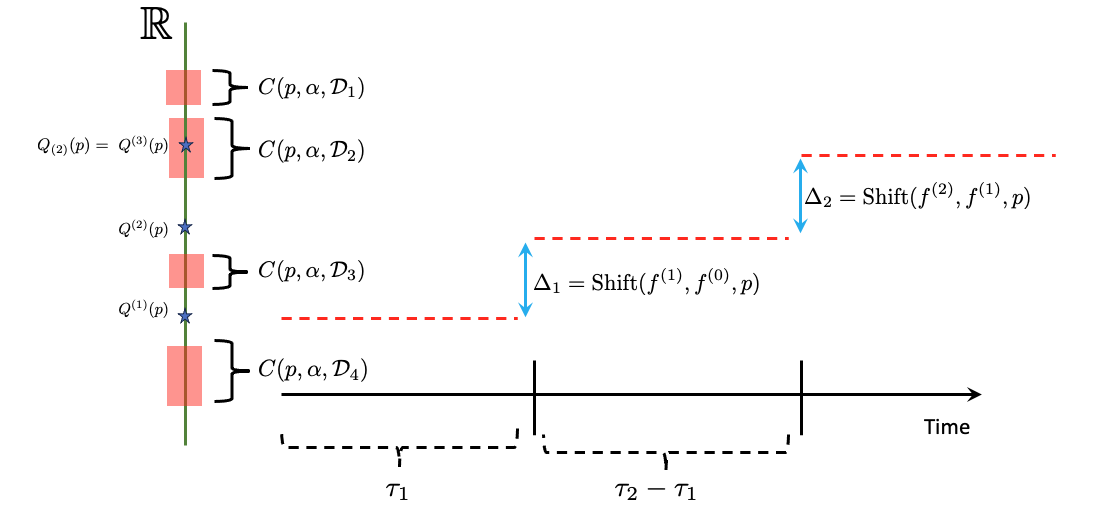
\includegraphics[width=0.9\linewidth]{anomaly/figs/separated_datasets.png}
%     \caption{An illustration of Assumption \ref{asumption_detectable} and \ref{defn:offline_datasets} on a stream with $2$ change-points ($H_T=2)$ and $K=4$ offline datasets. Assumption \ref{asumption_detectable} implies that the change-points on the stream are sufficiently far apart. Assumption \ref{defn:offline_datasets} implies that the $4$ CS do not intersect. Moreover, either the true quantile on the stream are outside the offline CS, i.e., $Q^{(1)}(p)$ and $Q^{(2)}(p)$ are not contained in any offline dataset's CS. Or, it is the case that the online quantile matches one of the offline dataset, i.e., $Q_{(2)}(p) = Q^{(3)}(p)$ in this example.}
%     \label{fig:separated_datasets_example}
% \end{figure}

}

\section{Proof for Theorem \ref{thm:core_theorem}, general case}
{\color{black}



To state performance guarantee of Algorithm \ref{alg:five}, we need a definition of a good event, which occurs with high probability.
\begin{definition}[Good event 4] 
Given a piece-wise stationary sequence $(S_t)_{t=1}^T := \Bigl(T,H_T, (\tau_c)_{c=0}^{H_T}, (f^{(c)})_{c=0}^{H_T}\Bigr)$, with the quantile functions of the $H_T+1$ different segments given by $(Q^{(c)}(\cdot))_{c=1}^{H_T}$ and $K$ offline datasets that are $(p,\alpha)$ separated according to Definition \ref{defn:offline_datasets}, let
% \begin{align}
% \begin{split}
%     \mathcal{E}_4 &:= \bigcap_{k=0}^{H_T} \bigcap_{s = \tau_{k}}^{\tau_{k+2}} \bigcap_{\tau'_k = s}^{\tau_{k+2}} \{ \Tilde{\theta}_{\tau_k:s} \in C_{\tau_k:s} \; \cap  \Tilde{\theta}_{s:\tau'_k} \in C_{s:\tau'_k}\}.\\
%     \end{split}

% \end{align}

\begin{align}
\begin{split}
    \gE_4 = \gG_2 \bigcap \underbrace{\bigcap_{p \in [0,1]}\bigcap_{j=1}^{K} \{ Q_{(k)}(p-u_{N_j}(\alpha)) \leq \widehat{Q}(p, \{ X_l^{(j)} \}_{l=1}^{N_j} ) \leq  Q_{(k)}(p+u_{N_j}(\alpha)) ) \}}_{\text{Offline dataset's CS contain true quantile}}   \\ \underbrace{\bigcap_{k=0}^{H_T}\bigcap_{t_1 = \tau_{k}}^{\tau_{k+1}} \bigcap_{t_2 = t_1 +1}^{\tau_{k+1}}   \bigg\{ \widehat{Q}(p-u_{t_2 - t_1}(\alpha), S_{t_1:t_2})  \leq Q^{(k)}(p) \leq \widehat{Q}(p-u_{t_2 - t_1}(\alpha), S_{t_1:t_2}) \bigg\}}_{\text{Online stream's CS contain true quantile}},
        \end{split}
                \label{eqn:good_event_4_defn}
\end{align}
where the $p$th quantile of the offline datasets $Q_{(l)}(p)$ are defined in Definition \ref{def:offline_quantile} and $\gG_2$ is defined in Equation (\ref{eqn:good_event_G}). 
\end{definition}

%
Event $\gE_4$ is the union of $\gE_2$ in Equation (\ref{eqn:good_event_2_defn}) for the online stream along with the event $\gE_3$ in Equation (\ref{eqn:good_event_3}) for the offline datasets. %The main result of this paper is stated below.

\begin{proposition}
    \begin{align*}
        \mathbb{P}[\gE_4] \geq 1- \alpha (K+2T)
    \end{align*}
    \label{prop:}
\end{proposition}
The proof follows similar to that of Proposition \ref{prop:good_event_2_prob}. 


%In this section, we specify the additional assumption on detectability, which combines the offline and online changes. 
As before, denote by $H_T$ as the number of change points, and the time-instants of change occuring at $1:= \tau_0 < \tau_1 < \tau_2 \cdots < \tau_{H_T} < \tau_{H_T+1}:= T+1$. We denote by the $k$th \emph{online stream} as the stationary samples $\{S_u : \tau_{k-1} \leq u < \tau_{k} \}$. 

For an offline dataset $j \in \{1,\cdots, K\}$ and the online stream $k$, $\Delta^{(j;k)} \geq 0$ denotes the shift between the $j$th offline dataset and the $k$th online stream. As before, similar to Theorem \ref{thm:online_shift}, for all $k \in [H_T]$, denote by $\Delta_{k} = \text{Shift} (f_{k},f_{k+1})$ to be the shift between the $k$th and $k-1$th online segment, and for $k \in [H_T]$ and $j \in [K]$, let $\Delta^{(j,k)} = \text{Shift} (f^{(k)},f_{(j)},p)$ be the shift between the $j$th offline dataset and the $k$th online segment. 
%The main detectability assumption in this section is the following which both Assumptions \ref{asumption_detectable} and \ref{as:offline_detectable}.

% \begin{assumption}[Offline assumption for every stream]
% We will assume that the number of offline dataset samples $N_1, \cdots, N_K$ and the number of online samples $(\tau_k - \tau_{k-1})_{k=1}^{H_T}$ satisfy  
% \begin{enumerate}
%     \item $\tau_{k} - \tau_{k-1} > D(\Delta_{k-1},\alpha) + D(\Delta_k, \alpha) + \max_{1 \leq j \leq K} D(\Delta^{(j;k)}, \alpha) \mathbf{1}(\Delta^{(j;k)} > 0)$
%     \item $N_j \geq \max_{1 \leq k \leq H_T} D(\Delta^{(j;k)}, \alpha) \mathbf{1}(\Delta^{(j;k)}>0)$
% \end{enumerate}
%     \label{as:offline_online_detect}
% \end{assumption}
% In words, the first assumption indicates that each stationary segment is large enough such that the change can be detected by using only the forward and backward confidence, and once a change is detected, the new segment can be matched with an offline dataset if the segment matches one of the offline datasets. The second assumption implies that if a given online segment's $p$th quantile is different from that of a offline dataset, then this change can be detected with high probability. 
% The detectability of this change is reliant on having sufficient number of samples in the offline dataset and thus the assumption is a lower bound on $N_j$. 
}

\begin{theorem*}[\ref{thm:core_theorem}] Let  $(S_t)_{t = 1}^T \sim \Bigl(T,H_T, (\tau_c)_{c=0}^{H_T}, (f_c)_{c=0}^{H_T}\Bigr)$  be a piece-wise stationary stream  satisfying Assumption \ref{asumption_detectable} and offline datasets  $\gD_1, \ldots, \gD_L$ satisfying  Assumption \ref{defn:offline_datasets}. Then, with probability at-least $1-(K+2T)\alpha$, for all times $T \in \mathbb{N}$, Algorithm \ref{alg:five} satisfies %{\em(i)} 
\begin{itemize}
    \item  $\text{FP} + \text{FN}  \leq \sum_{k=1}^{H_T} \left(D(\Delta_{k},\alpha) +  (1-\mathbf{1}_{\text{Match}_k})\max_{ j \in [K]} \left(\lceil \widehat{\tau}_j^{(k)}\rceil \mathbf{1}_{\text{Shift}(f^{(k)},f_{(j)},p) > 0}\right) \right)$ 
    \item Number of abstains less than 
    \begin{align*}
        \sum_{k=1}^{H_T} \Bigl[ &(1-\mathbf{1}_{\text{Match}_k}) 7 \sqrt{(\tau_k-\tau_{k-1}) \ln \left( \frac{1612}{\alpha^2} \ln(e(\tau_k-\tau_{k-1})) \right)}  \\ &+ \mathbf{1}_{\text{Match}_k}\left( 7 \sqrt{(N+T) \ln \left( \frac{1612\ln(e(N+T))}{\alpha^2} \right)}- 4 \sqrt{N \ln \left( \frac{1612\ln(eN)}{\alpha^2} \right)} \right) \\ &+  D(\Delta_{k},\alpha) +  \max_{ j \in [K]} \left(\lceil \widehat{\tau}_j^{(k)}\rceil \mathbf{1}_{\text{Shift}(f^{(k)},f_{(j)},p) > 0}\right)\Bigr],
    \end{align*}
\end{itemize}
where $\mathbf{1}_{\text{Match}_k} = \mathbf{1}_{Q^{(k)}(p) \in \{Q_{(1)}(p), \cdots, Q_{(K)}(p)\}}$, $Q^{(k)}(p)$ is the $p$th quantile of the $k$th segment of the online stream (Defn. \ref{def:piecewise}) and $Q_{(1)}(p), \cdots, Q_{(K)}(p)$ are the $p$th quantiles of the $K$ different offline datasets (Defn. \ref{definition:offline_dataset}).
\end{theorem*}




The proof structure follows a similar path as that of Theorem \ref{thm:online_shift}. Since Assumption \ref{asumption_detectable} holds, we know that Lemma \ref{lem:bdd_delay_change_induction} holds. Thus, we have that {\em(i)} there are no false positive change detections, and {\em(ii)} all changes are detected with a short detection delay. From the description of Algorithm \ref{alg:five}, we know that whenever a change is detected, a new instantiation of Algorithm \ref{alg:four} is started. Thus, the final result is obtained by summing the guarantees in Theorem \ref{thm:setting_3} over the $k$ online segments in addition to the delay taken to detect changes. 
The delay to detect changes are bounded by using Proposition \ref{prop:delay_bound} and Assumption \ref{asumption_detectable}, similar to that done in Theorem \ref{thm:online_shift}. 


% We will prove through induction, that under the good event $\mathcal{E}_4$ and Assumption \ref{as:offline_online_detect},  and {\em(iii)} if an online segment matches an offline dataset, then the match is identified quickly. If on the other hand a segment does not match any offline dataset, then the number of additional mistakes incurred is small. Concretely, the following is the key structural lemma of Algorithm \ref{alg:five}. 

% In order to state the lemma, we recall the notations that we set in the proof of Lemma \ref{lem:bdd_delay_change_induction}. As before, denote by $\tau_1 < \tau_2 \cdots < \tau_k < \tau_{k+1}$ be the set of times at which a true-change occurs. For each $k \in \{1, \cdots, H_T\}$, denote by $\tau_k^{'}$ as the time at which Algorithm \ref{alg:five} detects a change for the $k$th time.

% \begin{lemma}[No false change detections and bounded delay for identifying change and matching offline datasets]
%         Under the event $\mathcal{E}_4$, if Assumption \ref{as:offline_online_detect} holds, then for all $k \in \{1, \cdots, H_T\}$, 
%     \begin{itemize}
%         \item  $\tau_k^{'} \geq \tau_k$, and
%         \item $\tau_k^{'} - \tau_k \leq D(\Delta_k, \alpha)$.
%     \end{itemize}
%     \label{lem:bdd_delay_change_induction_general}
% \end{lemma}

% Before we prove the lemma, we show how this concludes the proof of Theorem \ref{thm:core_theorem}.

\begin{proof}[Proof of Theorem \ref{thm:core_theorem}]
    Theorem 6 is the joint result of theorems \ref{thm:online_shift} and \ref{thm:setting_3}. As in Theorem \ref{thm:online_shift}, Lemma \ref{lem:bdd_delay_change_induction} implies that at time $\tau'_k < \tau_{k+1}$, a new instantiation of Algorithm \ref{alg:four} is started. Theorem \ref{thm:setting_3} states that in the time interval $[\tau'_k, \tau_{k+1}]$, the $k$th online segment incurs a total number of mistakes bounded by the guarantee in Theorem \ref{thm:setting_3} for a time horizon $\tau_{k+1} - \tau'_{k}$. Concretely, in the time-interval $[\tau'_k, \tau_{k+1}]$, the sum of FP and FN is bounded above by $0$ in the event  $\mathbf{1}_{\text{Match}_k}$ holds, and by $\max_{ j \in [K]} \left(\lceil \widehat{\tau}_j^{(k)}\rceil \mathbf{1}_{\text{Shift}(f^{(k)},f_{(j)},p) > 0}\right) $ in the case when $\mathbf{1}_{\text{Match}_k}$ does not hold. %In other words, the sum of FP and FN in the time interval $\tau_{k+1} - \tau_{k}^{'}$ is at-most $\max_{1\leq j \leq K} D(\Delta^{(j;k)}, \alpha)\mathbf{1}(\Delta^{(j;k)} > 0)$. 
    Similarly, the number of abstains in the time-interval $\tau_{k+1} - \tau_{k}^{'}$ is given by the guarantee of Theorem \ref{thm:setting_3}. Now, summing over the $H_T$ different online segments yields the result. 
    
    For any segment $k \in [1, \ldots, H_T]$,  we have 
    \begin{itemize}
        \item $\text{FP}_k + \text{FN}_k  \leq D(\Delta_{k},\alpha) +   1-\mathbf{1}_{\text{Match}_k})\max_{ j \in [K]} \left(\lceil \widehat{\tau}_j^{(k)}\rceil \mathbf{1}_{\text{Shift}(f^{(k)},f_{(j)},p) > 0}\right)$ where the first term is from detection delay in detecting the change (Proposition \ref{prop:delay_bound}) and the second term from Theorem \ref{thm:setting_3}.
        \item If $Q^{(k)}(p)$ matches one of the dataset $\{Q_{(1)}(p), \cdots, Q_{(K)}(p)\}$, then under event $\gG_2$, number of abstains is at-most
        \begin{align*}
           D(\Delta_k, \alpha)+ \max_{ j \in [K]} \left(\lceil \widehat{\tau}_j^{(k)}\rceil \mathbf{1}_{\text{Shift}(f^{(k)},f_{(j)},p) > 0}\right) + 7 \sqrt{(N+\tau_k - \tau_{k-1}) \ln \left( \frac{1612\ln(e(N+\tau_k - \tau_{k-1}))}{\alpha^2} \right)} \\ - 7 \sqrt{N \ln \left( \frac{1612\ln(eN)}{\alpha^2} \right)},
        \end{align*}
        by Theorem \ref{thm:core_theorem}, case $\Delta = 0$.
        \item  If $Q^{(k)}(p)$ matches none of the datasets:
        \[ \text{Abstains} \leq   D(\Delta_k, \alpha)+ \max_{ j \in [K]} \left(\lceil \widehat{\tau}_j^{(k)}\rceil \mathbf{1}_{\text{Shift}(f^{(k)},f_{(j)},p) > 0}\right) + 7 \sqrt{(\tau_k - \tau_{k-1}) \ln \left( \frac{1612\ln(e(\tau_k - \tau_{k-1})))}{\alpha^2} \right)} 
        \]
        by theorem \ref{thm:core_theorem}, case $\Delta > 0$.
    \end{itemize}
The term of $D(\Delta_k, \alpha)$ always shows in all three equations above as that is the amount of time taken for the $k$th change-point to be detected and thus all decisions made during the times of change can potentially lead to mistakes and abstains. Combining the piece-wise results together, we have 
    \begin{align*}
    \text{FP} + \text{FN} \;  \leq \; & \sum_{k=1}^{H_T}D(\Delta_{k},\alpha) + (1-\mathbf{1}_{\text{Match}_k})  \max_{ j \in [K]} \left(\lceil \widehat{\tau}_j^{(k)}\rceil \mathbf{1}_{\text{Shift}(f^{(k)},f_{(j)},p) > 0}\right) 
        \end{align*}
        Similarly, summing over the $H_T$ online segments gives the bound on the number of abstains. 
         % \text{Abstains} \;  \leq \;  &  \sum_{k=1}^{H_t} \Bigl[ (1-\mathbf{1}_{\text{Match}_k}) \mathcal{O}(\sqrt{\tau_k - \tau_{k-1}}) \\ &+ \mathbf{1}_{\text{Match}_k}\left(\gO(\sqrt{N+(\tau_k-\tau_{k-1})} - \sqrt{N}) \right) \\ &+  D(\Delta_{k},\alpha) \Bigr],

\end{proof}

% --------------------------------------------------

% \subsection{Necessity of Assumption \ref{asumption_detectable}  }

% The core of our result requires that the changes are not too often, i.e., there is sufficient gap between changes, quantified precisely in Assumption \ref{asumption_detectable}. We remark that these assumptions are standard in the study of online decision making under non-stationarity \cite{liu2018change, JMLR:v23:20-1384}. This assumption ensures that all changes are detected. However, it is an interesting question to have a non-trivial analysis of dynamic decision making algorithms without assuming that each stationary environment is sufficiently long (Conclusion section of \cite{JMLR:v23:20-1384}). 

\section{Additional Related Works}
\label{app:related}

\paragraph{Online anomaly detection works} There exist works that focuses on other aspects of online anomaly detection. \cite{zhu2023meter} models online concept drift via an ensemble of models.   \cite{nardi2022anomaly} tackles modeling for online AD in a Federated setting. \cite{bhatia2022memstream} studies the low-memory constraint of online AD, and \cite{goyal2020drocc} focuses on efficiently modeling multi-dimensional data. A survey of methodologies of data modelling for AD can be found in the surveys of \cite{chandola2009anomaly, ruff2021unifying, pang2021deep}. Our work differs from these works in setting: we focus on dynamic thresholding of anomaly scores without having access or ability to retrain the underlying AD algorithm.

\paragraph{Threshold learning} Using score thresholds to make binary decision of seeking labels from human experts are studied in active learning \cite{balcan2007margin, zhang2016online,vishwakarma2023promises}. However, active learning does not have a concept of mistakes and is thus have different desiderata compared to our study. 

\section{Additional experiments and experiment details}
\label{app:exp1}

\subsection{Synthetic experiments}
We conduct our synthetic experiments for 1000 trails on streams each of length 1000. The normal distribution online streams are synthesized with parameters sampled uniformly form $[0, 10]$ for mean and $[0.2, 2]$ for variance. The Pareto distributions' parameters are sample uniformly from $[1,3]$ for $b$, $[0,10]$ for mean, and $[0.2,2]$ for scale. To synthesize distribution shifts, we sample a duration for each stationary piece from a Poisson distribution with $\lambda = 300$. To simulate datasets, we prepare $L=5$ offline datasets each of size $N=5000$; the online stream can be generated from either one of the dataset distributions or a random one with uniform probability. The range of these parameters are chosen to simulate real world anomaly score data. The code to generate the synthetic dataset as well as implementations of our algorithms will be open sourced.


\begin{table}[h!]
    \centering

    % \begin{tabular}{c c |c  c |c c}
    % \toprule
    %   & & \multicolumn{2}{|c|}{Normal} & \multicolumn{2}{|c}{Pareto} \\
    %   shift  & data   &  Abs. (\%) & Mis. (\%) &  Abs. (\%) & Mis. (\%)\\
    %   \midrule 
    %  x & x &  18.1 \plusminus{1.1} &  0 \plusminus{0} & 17.8 \plusminus{7.4} & .03 \plusminus{.01}\\
    %  \checkmark & x &   41.7 \plusminus{12.1} &  .05 \plusminus{0} &  51.9 \plusminus{35.0} & .51 \plusminus{.18}\\
    %  x & \checkmark  &  14.3 \plusminus{2.6} &  0 \plusminus{.01}& 16.8 \plusminus{4.7} & .06 \plusminus{.04} \\
    %  \checkmark  & \checkmark  & 32.9 \plusminus{7.1} &  .05 \plusminus{.03} & 24.3 \plusminus{5.2} &  .33 \plusminus{ .41 }\\
    % \bottomrule
    % \end{tabular}
    \begin{tabular}{c c |c c}
\toprule
  & & \multicolumn{2}{|c}{Pareto} \\
  shift & data & Abs. (\%) & Mis. (\%) \\
\midrule
 x & x & 17.8 \plusminus{7.4} & .03 \plusminus{.01} \\
 \checkmark & x & 51.9 \plusminus{35.0} & .51 \plusminus{.18} \\
 x & \checkmark & 16.8 \plusminus{4.7} & .06 \plusminus{.04} \\
 \checkmark & \checkmark & 24.3 \plusminus{5.2} & .33 \plusminus{.41} \\
\bottomrule
\end{tabular}

    \caption{Results of our algorithms on synthetic stream dataset generated from Pareto distribution.}
    \label{tab:synthetic_appendix}
\end{table}

\subsection{Case study of real AD application}
In this section we provide details on our real data experiments. We run Algorithms \ref{alg:two} and \ref{alg:five} on two large scale datasets {\ttfamily DS1} and {\ttfamily DS2} obtained from monitoring two large cloud computing services. Each dataset is a stream of anomaly scores obtained by applying a single anomaly detection algorithm. On these datasets, we run our two general algorithms, Algorithm \ref{alg:two} and \ref{alg:five} with $p = 1 - 10^{-6}$ and $\alpha = 10^{-6}$. Algorithm \ref{alg:five} can use offline datasets. In order to create them, we sampled 50 streams randomly that had length at-least $20,000$ in each of the two datasets. From this collection of $100$ streams, we sub-selected $37$ and $23$ streams from datasets {\ttfamily DS1} and {\ttfamily DS2} respectively such that no two datasets in this collection of $60$ streams overlapped. This is so that Assumption 6.1 is satisfied by the offline dataset. 

The description of the rest of the dataset on which we run the online algorithms is in Table \ref{tab:real_data_stats}. In addition, we also run {\ttfamily DSpot} \cite{siffer2017anomaly} with $p = 1 - 10^{-6}$ and set {\ttfamily num-init} to $500$ and {\ttfamily depth} to $100$ on the online algorithm dataset. All other parameters of {\ttfamily DSpot} was set to the suggested values in \cite{siffer2017anomaly}. In addition to these, we also compare against two static baselines of using the first $500$ and $100$ samples respectively and set the threshold as the max of the observed samples. This threshold is not changed since. 

The results of this experiment are reported in Table \ref{tab:real_data}. From this table, we can see that incorporating offline data reduces the number of abstains for both datasets without changing the volume of anomalies raised. This shows that when there are offline datasets available to the algorithm, the online performance is improved. 


\begin{table}[h!]
    \centering
    \begin{tabular}{c|c|c|c}
    \toprule
     & Num. of Streams & Average stream length &  Total num samples   \\ \midrule 
{DS1}  & $8377$ & $10925.4$ & $91521785$\\ \midrule
{DS2}  & $9657$ &  $10855.6$ & $104832532$\\
         \bottomrule
    \end{tabular}
    \caption{Summary of data properties for real world AD case study.}
    \label{tab:real_data_stats}
\end{table}


\begin{table}[h!]
    \centering

    \begin{tabular}{c|c|c|c| c| c|c}
    \toprule
                &  & Algo 3 & Algo 5 &  DSpot & $\tau^{(1)}$  & $\tau^{(2)}$  \\
        \midrule
         \multirow{2}{*}{DS1}  & Abstains $\downarrow$ & $13.6\%$ & $11.2\%$ & $1.2\%$ & $1.16\%$ & $0.05\%$\\
          & Anomaly $\downarrow$ & $\mathbf{.008\%}$ & {$\mathbf{.008\%}$} & $2.9\%$ & $0.02\%$ & $0.95\%$\\
          \midrule
         \multirow{2}{*}{DS2}  & Abstains $\downarrow$ & $13.3\%$ & $9.9\%$ & $1.3\%$& $1.25\%$ & $1.08\%$   \\
          & Anomaly $\downarrow$ & $.006\%$ & $\mathbf{.005\%}$ & $3.9\%$ & $0.07\%$ & $0.06\%$ \\
         \bottomrule
    \end{tabular}
    
    \caption{Case study performance. All baseline algorithms report anomaly rates much higher than the targeted $10^{-6}$, overwhelming the alarm system. By incorporating offline datasets, we are able to further decrease abstains and achieve a lower rate of reported anomaly. 
    }
    \label{tab:real_data}
\end{table}

\subsection{Additional experiment on open-source datasets}

We include additional experiments as follows. With the same underlying AD scoring algorithm (isolation forest for ForestCover, and a 3-layer MLP for Mammography), our confidence sequence algorithm (Algorithm \ref{alg:marginal_decision} in paper) can achieve a higher F1 score and fewer mistakes, with similar or less number of abstains, compared to a static threshold. This further demonstrates that our thresholding algorithm improves performance across datasets and base anomaly scoring algorithms.


\begin{table}[h!]
    \centering
    \begin{tabular}{ccc|cc}
        \toprule
       &\multicolumn{2}{c}{ForestCover (first 1500 as holdout)} & \multicolumn{2}{c}{Mammography (first 300 as holdout)} \\
        \midrule
        & Ours & Static Threshold & Ours & Static Threshold \\
        \midrule
        Abstain \% & 1.5\% & 1.5\% & 2.1\% & 5\% \\
        FP + FN & 645 & 1603 & 56 & 83 \\
        F1 & 0.39 & 0.33 & 0.51 & 0.43 \\
        \bottomrule
    \end{tabular}
    \caption{Performance comparison of algorithms on ForestCover and Mammography datasets}
    \label{tab:performance}
\end{table}



\section{Proof of Lower Bound}
\label{sec:lower_bound_proof}
The proof is based on the classical hypothesis testing lower bounds due to Neyman and Pearson. Throughout this section, we will fix a $T \in \mathbb{N}$ sufficiently large and let $\mathbb{P}_0 := N(0,1)$  be the standard normal distribution and $\mathbb{P}_{1} := N(\frac{1}{\sqrt{T}},1)$ as an unit variance normal distribution with mean $1/\sqrt{T}$. 

\begin{theorem}[Neyman-Pearson]
For any $T \in \mathbb{N}$, given $T$ i.i.d.. samples $S_{1:T}$, we want to distinguish between the two hypothesis $H_0: S_{1:T} \sim \mathbb{N}(0,1)$ or $H_1: S_{1:T} \sim \mathcal{N}(1/\sqrt{T},1)$. Then, for any measurable function $\mathcal{A} : \mathbb{R}^T \to \{0,1\}$, 
\begin{align*}
   \max( \mathbb{P}_0[\mathcal{A}(S_{1:T}=1], \mathbb{P}_0[\mathcal{A}(S_{1:T}=1]) \geq \frac{1}{4} \exp(-\frac{1}{2}),
\end{align*}
    where $\mathbb{P}_{i}$ for $i \in \{0,1\}$ is the proabability distribution under hypothesis $H_i$.
    \label{thm:neyman_pearson}
\end{theorem}

\begin{lemma}
    For every $p \in (0,1)$, there exists a constant $C_p \in (0,\infty)$ depending only on $p$, such that for $S \sim {N}(0,1)$
    \begin{align*}
        \mathbb{P}[S \in (Q^{(0)}(p), Q^{(1)}(p))] \geq \frac{C_p}{\sqrt{T}},
    \end{align*}
    where $Q^{(0)}(p)$ is the $p$th quantile of a $N(0,1)$ distribution and $Q^{(1)}(p)$ is the quantile of a $N(\frac{1}{\sqrt{T}},1)$ distribution.
    \label{lem:cp_lb}
\end{lemma}

Now, a standard Chernoff bound gives the following result.
\begin{lemma}[Chernoff bound]
Let $T \in \mathbb{N}$ and suppose $S_{1:T}$ are i.i.d., $N(0,1)$ random variables. Let $p \in (0,1)$. Then, 
\begin{align}
    \mathbb{P}\left[ \sum_{t=1}^T \mathbf{1}_{S_t \in (Q^{(0}(p), Q^{(1)}(p))} \leq \frac{C_p\sqrt{T}}{2} \right] \leq \exp \left( \frac{\sqrt{T}}{8} \right),
\end{align}
where $C_p$ is from Lemma \ref{lem:cp_lb}.
    \label{lem:lb_chernoff}
\end{lemma}

\begin{theorem}[Main lower bound]
Denote by two distributions  $\mathbb{P}_0 := N(0,1)$ and $\mathbb{P}_{1} := N(\frac{1}{\sqrt{T}},1)$ as unit variance guassians with means $0$ and $\frac{1}{\sqrt{T}}$ respectively. For $i \in \{0,1\}$, denote by $Q^{(i)}(p)$ as the $p$th quantile of distribution $\mathbb{P}_i$. For a threshold $\theta \in \mathbb{R}$ and sample $x \in \mathbb{R}$, denote by the indicator function $\widehat{Y}_t^{(\theta)}(x) := \mathbf{1}(x \geq \theta)$. Similarly, denote by the indicator function $Y_t^{(i)}(x) = \mathbf{1}(x \geq Q^{(i)})$ for $i \in \{0,1\}$. Let $\mathcal{A}: \mathbb{R}^T \to \{0,1\}$ be any measurable hypothesis testing function. Then, there exists $i \in \{0,1\}$ such that when $S_{1:T}$ are i.i.d. with distribution $\mathbb{P}_i$, then with probability at-least $\frac{1}{8} -  \exp \left( \frac{\sqrt{T}}{8} \right)$,
    \begin{align*}
 \sum_{t=1}^T \mathbf{1} ( \widehat{Y}_t^{(Q^{(\mathcal{A}(S_{1:T}))}(p))}(S_t) \neq Y_t^{(i)}(S_t) ) \geq C_p \sqrt{T},
    \end{align*}
where $C_p$ is from Lemma \ref{lem:cp_lb}.
    \label{thm:main_lower_bound}
\end{theorem}
In words, the above theorem states that even when the true distribution is known to be one of two possibilities and the optimal threshold is chosen using any measurable function, $O(\sqrt{T})$ mistakes is un-avoidable. 

\begin{proof}
Pick $\mathcal{A}: \mathbb{R}^T \to \{0,1\}$ by a measurable function that tests the hypothesis $H_0: S_{1:T}$ are i.i.d. with distribution $\mathbb{P}_0$ and $H_1: S_{1:T}$ are i.i.d. with distribution $\mathbb{P}_1$. From Theorem \ref{thm:neyman_pearson}, we know that for this given test $\mathcal{A}$, there exists $i \in \{0,1\}$ such that
\begin{align}
\mathbb{P}_i[\mathcal{A}(S_{1:T}) \neq i] \geq \frac{1}{8}.
\end{align}
Without loss of generality, lets suppose $i = 0$, i.e., given a hypothesis test $\mathcal{A}$, $\mathbb{P}_0[\mathcal{A}(S_{1:T}) \neq 0] \geq \frac{1}{8}$. We will show in the rest of the proof that for this $\mathcal{A}$, if $S_{1:T}$ are i.i.d. with distribution $\mathbb{P}_0$, $ \sum_{t=1}^T \mathbf{1} ( \widehat{Y}_t^{(Q^{(\mathcal{A}(S_{1:T}))}(p))} \neq Y_t^{(0)} ) \geq C_p \sqrt{T}$ holds with probability at-least $\frac{1}{8} -  \exp \left( \frac{\sqrt{T}}{8} \right)$.

To do so, let $S_{1:T}$ be i.i.d. $\mathbb{P}_0$. From Lemma \ref{lem:lb_chernoff}, we know that 
\begin{align*}
             \mathbb{P}_0\left[ \sum_{t=1}^T \mathbf{1}_{S_t \in (Q^{(0}(p), Q^{(1)}(p))} \leq \frac{C_p\sqrt{T}}{2} \right] \leq \exp \left( \frac{\sqrt{T}}{8} \right). 
\end{align*}
Thus, from an union bound, we know that for the given $\mathcal{A}$,
\begin{align*}
    \mathbb{P}_0 \left[ \underbrace{\mathcal{A}(S_{1:T}) \neq 0,  \sum_{t=1}^T \mathbf{1}_{S_t \in (Q^{(0}(p), Q^{(1)}(p))} \geq \frac{C_p\sqrt{T}}{2}  }_{\text{Event }\mathcal{H}}\right] \geq \frac{1}{8} - \exp \left( \frac{\sqrt{T}}{8} \right). 
\end{align*}

Observe that under event $\mathcal{H}$, for all $x \in \mathbb{R}$, we have the equality

\begin{align*}
     \mathbf{1} ( \widehat{Y}_t^{(\mathcal{A}(S_{1:T}))}(x) \neq Y_t^{(0)}(x) ) = \mathbf{1} (x \in (Q^{(0)}(p), Q^{(1)}(p)).
\end{align*}
Thus, under event $\mathcal{H}$, we have 
\begin{align*}
    \sum_{t=1}^T \mathbf{1} ( \widehat{Y}_t^{(\mathcal{A}(S_{1:T}))}(S_t) \neq Y_t^{(0)}(S_t) ) = \sum_{t=1}^T \mathbf{1}_{S_t \in (Q^{(0}(p), Q^{(1)}(p))} \geq \frac{C_p\sqrt{T}}{2},
\end{align*}
holding with probability at-least $\frac{1}{8} - \exp \left( \frac{\sqrt{T}}{8} \right).$
\end{proof}

%\subsection{Discussion of the lower bound}

The theorem asserts that if an algorithm does not abstain, then even in a stationary stream, $O(\sqrt{T})$ mistakes will occur with high probability. 


%\bibliographystyle{plain}
%\bibliography{ref}

